\documentclass[svgnames, table, smaller]{beamer}
\usepackage{subfigure}
\usepackage[latin1]{inputenc}
\usepackage{epstopdf}
\usepackage{multicol}
\usepackage{multirow}
\usepackage{amsthm}
\usepackage{amsmath, amssymb}
\usepackage{amsfonts}
\usepackage[noend]{algorithmic}
\usepackage[lined, boxed]{algorithm2e} 
%\usepackage{cite} 
\newcommand{\newblock}{}
%\usepackage[square, sort]{natbib}
%\usepackage{subfig}

\newtheorem*{conjecture}{Conjecture}


\usetheme{Warsaw}
\title[Learning Patterns of Expert Behaviour In Design]{LEARNING PATTERNS OF EXPERT BEHAVIOUR IN MULTI-OBJECTIVE DESIGN}
\author[Kushlendra Mishra]{Kushlendra Mishra \\ Y8111018 \\{\small   Supervisor - Prof. Amitabha Mukerjee}}

\institute[IIT Kanpur]{DEPARTMENT OF COMPUTER SCIENCE AND ENGINEERING,\\ INDIAN INSTITUTE OF TECHNOLOGY KANPUR}
\date{17 January, 2011}
\begin{document}

\begin{frame}
\titlepage
\end{frame}

\begin{frame}
  \frametitle{Outline}
  \tableofcontents
\end{frame}   

\section{Introduction}

\subsection{Expert behaviour}

\begin{frame}
  \frametitle{Expert behaviour}

  \begin{itemize}
  \item Experts are able to think effectively about problems.
  \item Experience and practice lead to effective organization of
    knowledge, that leads to expertise.
  \item Expert knowledge is `conditionalised' to the context of
    applicability.
  \item With experience, knowledge is chunked into larger units based on
    functional characteristics.
  \item Chunking leads to abstraction.
  \item Expert behaviour in design:
    \begin{itemize}
    \item Framing the problem.
    \item Fixing a principal solution.
    \item Identify the aspects of the design problem that need attention.
    \item Modify the principal solution according to the design requirements.
    \end{itemize}
  \end{itemize}
\end{frame}

\begin{frame}
  \frametitle{Previous work and goals}
  \begin{itemize}
  \item  \cite{moss04} Uses prior knowledge.
  \item \cite{deb10} - Human based extraction of design implicit design principles.
  \item  \cite{mukerjee09} - Symbols emerge from experience.
  \end{itemize}
  
  \begin{itemize}
  \item Explore discovery of chunks.
  \end{itemize}
    
\end{frame}      


\subsection{Chunk dimensionality conjecture}

\begin{frame}
  \frametitle{Chunk dimensionality conjecture}
  {\allowdisplaybreaks
    \begin{conjecture}[Chunk dimensionality conjecture]\label{cdconjecture}
      Given a multi-objective optimization problem with a decision variable $x
      \in \Sigma$, where $\Sigma$ is the decision space,
      
      \pause

% For
%   $d$-objective multi-objective optimization problem with a $D$ dimensional
%   decision space,

      \begin{enumerate}[(a)]
      \item chunks emerge from a high-dimensional decision space
        $\mathbb{R}^{D}$ as clusters among the better performing combinations,
        \pause
        
      \item chunks reflect a lower dimensionality than the embedding space,
        i.e.  chunks are manifolds of dimension $d_{c}$, $d_{c} < D$,
        \pause
        
      \item for multi-objective decision problems with $d+1$ objectives ($d
        \ll D$), the better performing combinations are to be found on the
        non-dominated (pareto) frontier which is a $d$-dimensional manifold
        in the objective space, and
        \pause

      \item if the objective function that maps the decision space to the
        objective space is continuous and well-behaved, this would result in
        chunks that have a dimensionality $d_{c} = \textbf{o}(d)$,
        i.e. $d_{c} = kd$, where $k-1$ is vanishingly small.
        
      \end{enumerate}
    \end{conjecture}
  }

\end{frame}

\section{Proposed methodology}

\subsection{Overview}

\begin{frame}
  \frametitle{Overview of the chunking process}
  \begin{figure}[ht]\begin{center}
      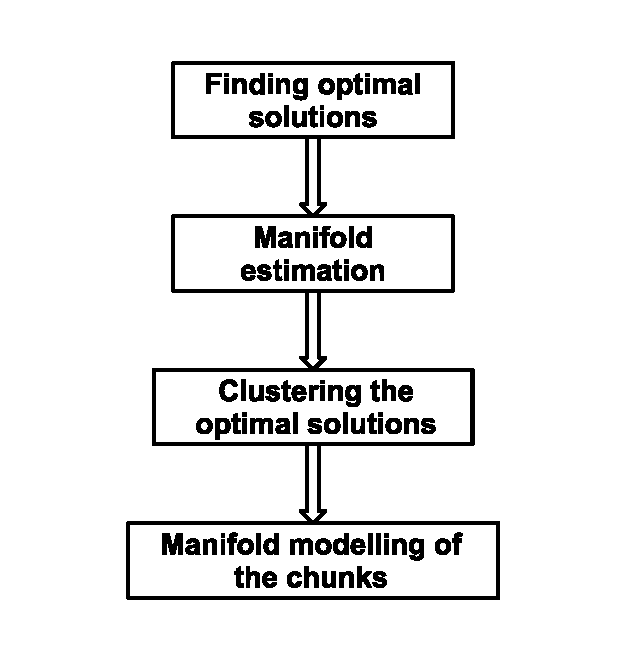
\includegraphics[width=60mm, height=60mm]{dia/overview.eps}
      \label{overview}
    \end{center}\end{figure}
\end{frame}



\subsection{Manifold estimation}

\begin{frame}
  \frametitle{Estimating the pareto-front manifold}
  
  \begin{itemize}
  \item Dimensionality reduction:
    \begin{enumerate}
    \item Linear techniques: PCA.
    \item Non-linear techniques: LLE, Isomap$^*$, Laplacian Eigenmaps.
    \end{enumerate}
  \end{itemize}
\end{frame}


\subsection{Clustering}


\begin{frame}
  \frametitle{3-d Isomap embedding of the BDCPMM pareto-front}

  \begin{figure}[ht]
    \begin{center}
      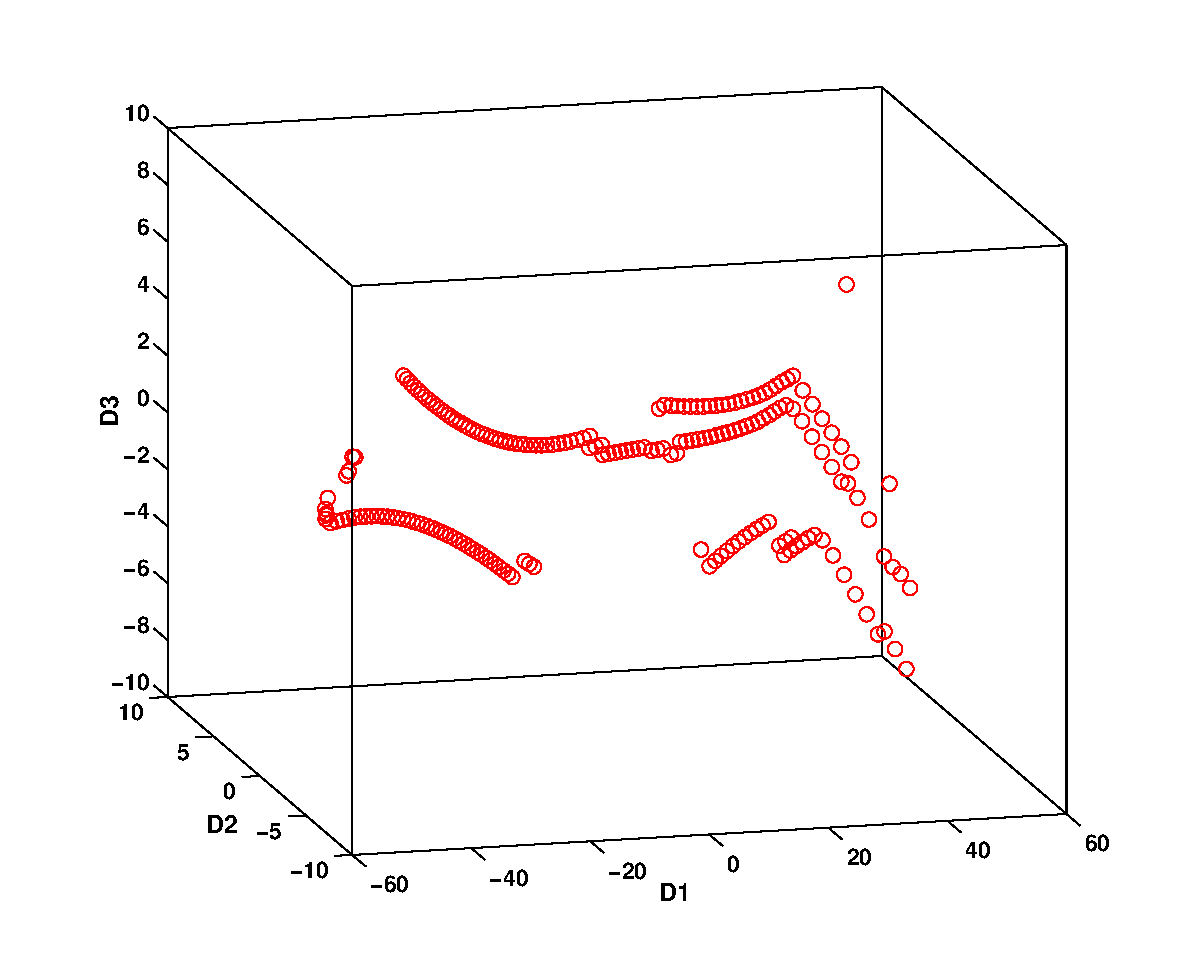
\includegraphics[width=65mm, height=55mm]{diagrams/bdcpmiso3.eps} 
      \label{bdcpmiso3}
    \end{center}
  \end{figure}


\end{frame}


\begin{frame}
  \frametitle{Clusters in BDCPMM problem decision space}

\end{frame}

\begin{frame}[allowframebreaks]
  \frametitle{Clustering the optimal solution set}
  
  \begin{itemize}
  \item Clustering in the objective-decision variable space to group solutions
    which are functionally similar.
  \item A density based clustering algorithm similar to DBSCAN is used.
  \item {\em Core objects} and {\em Density connectivity}.
  \item Build a graph based on density connectivity.

  \item Steps of the algorithm:
    \begin{enumerate}
    \item Find $MinPoints$ nearest neighbors of each point and sort in the
      increasing order of distance to the point.
    \item A point $p$ is connected to a point $n$ at the top of its nearest
      neighbor list only if its distance is {\em similar} to the average
      neighbor distance in the component the nearest number $n$ belongs to.
    \item Process repeated for $MinPoints$ iterations.
    \end{enumerate}
  \item The size and number of components can be controlled through the $k$ 
    parameter.
  \end{itemize}
\end{frame}


\section{Experiments}

\begin{frame}
  \frametitle{Experiments}

{\tiny
\begin{table}[!ht]
  \centering
  \begin{tabular}{|c|c|c|c|c|c|}
    \hline
    \multirow{2}{*}{Design problem} & \multirow{2}{*}{$D$} & \multirow{2}{*}{Cont. variables} & \multirow{2}{*}{$d+1$}  & \multicolumn{2}{c|}{Cluster dimensionality} \\
    \cline{5-6} 
    &&&&Dimensionality & No. of clusters \\
    \hline
    \multirow{2}{*}{BDCPM design} & \multirow{2}{*}{5} & \multirow{2}{*}{0} & \multirow{2}{*}{2} & 1 & 4 \\
    \cline{5-6} 
    &&&&2 & 1 \\
    \hline
    Gearbox design (A) & 11 &10 & 2 & 1 & 11 \\
    \hline
    Gearbox design (B) & 29 & 10 & 3 & 2 & 7 \\
    \hline
    Clutch brake design & 5 & 0 & 2 & 1 & 5 \\
    \hline
    Welded beam design & 4 & 4 & 2 & 1 & 5 \\

    % &&& 2 & 1\\
    \hline
    % \multicolumn{1}{|c|}{\multirow{2}{*}{\textbf{C}}} & 0.435 & 0.897 & -0.066 & -0.003 \\ \cline{2-5}
    % \multicolumn{1}{|c|}{}& 0 & 0.006 & 0.04 & 0.999\\
    % \hline
  \end{tabular}
  \label{expSummary}
\end{table}
}

  

\end{frame}

\subsection{A. Brushless DC permanent magnet motor design Problem}

\begin{frame}[allowframebreaks]
  \frametitle{Brushless DC permanent magnet motor design Problem}


  \begin{itemize}
  \item Two objectives:
    \begin{enumerate}[(i)]
    \item Minimize the cost, and
    \item Maximize the peak torque.
    \end{enumerate}
  \end{itemize}
  

  \begin{figure}[ht]
    \begin{center}
      \subfigure[BDCPMM Stator lamination.] {
        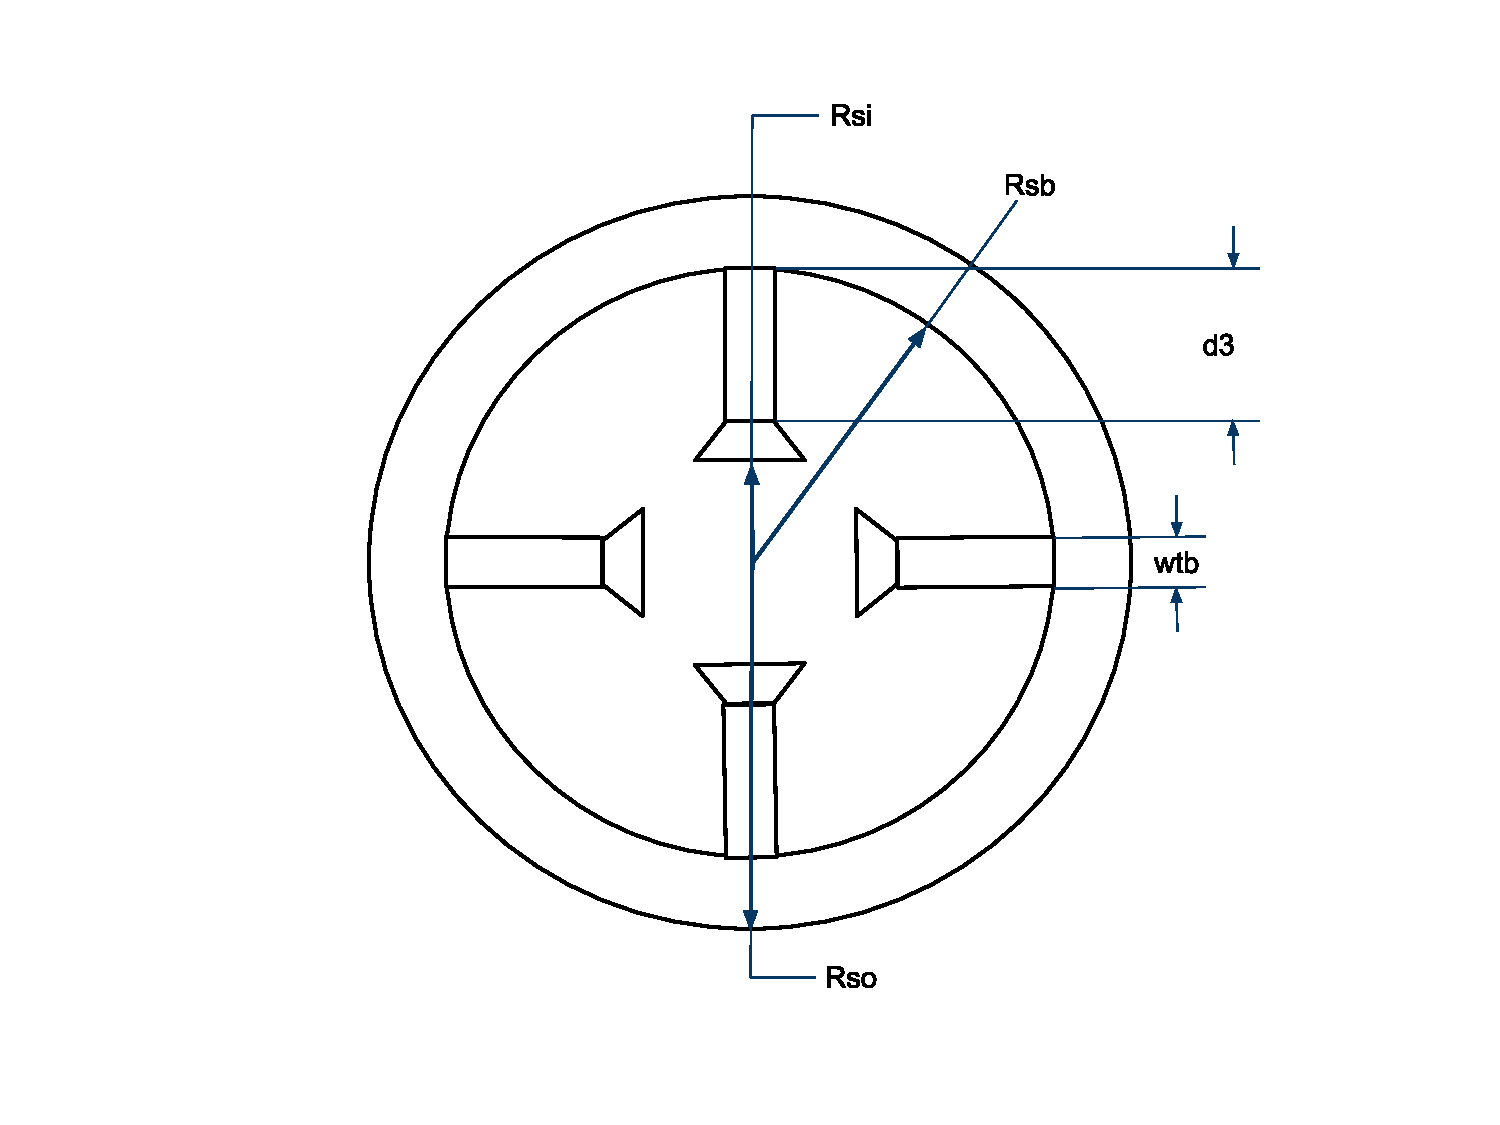
\includegraphics[width=41mm, height=30mm] {diagrams/bdcpmStator.eps}
        \label{isoRVbdcpmAll}
      }
      \subfigure[BDCPMM Rotor.] {
        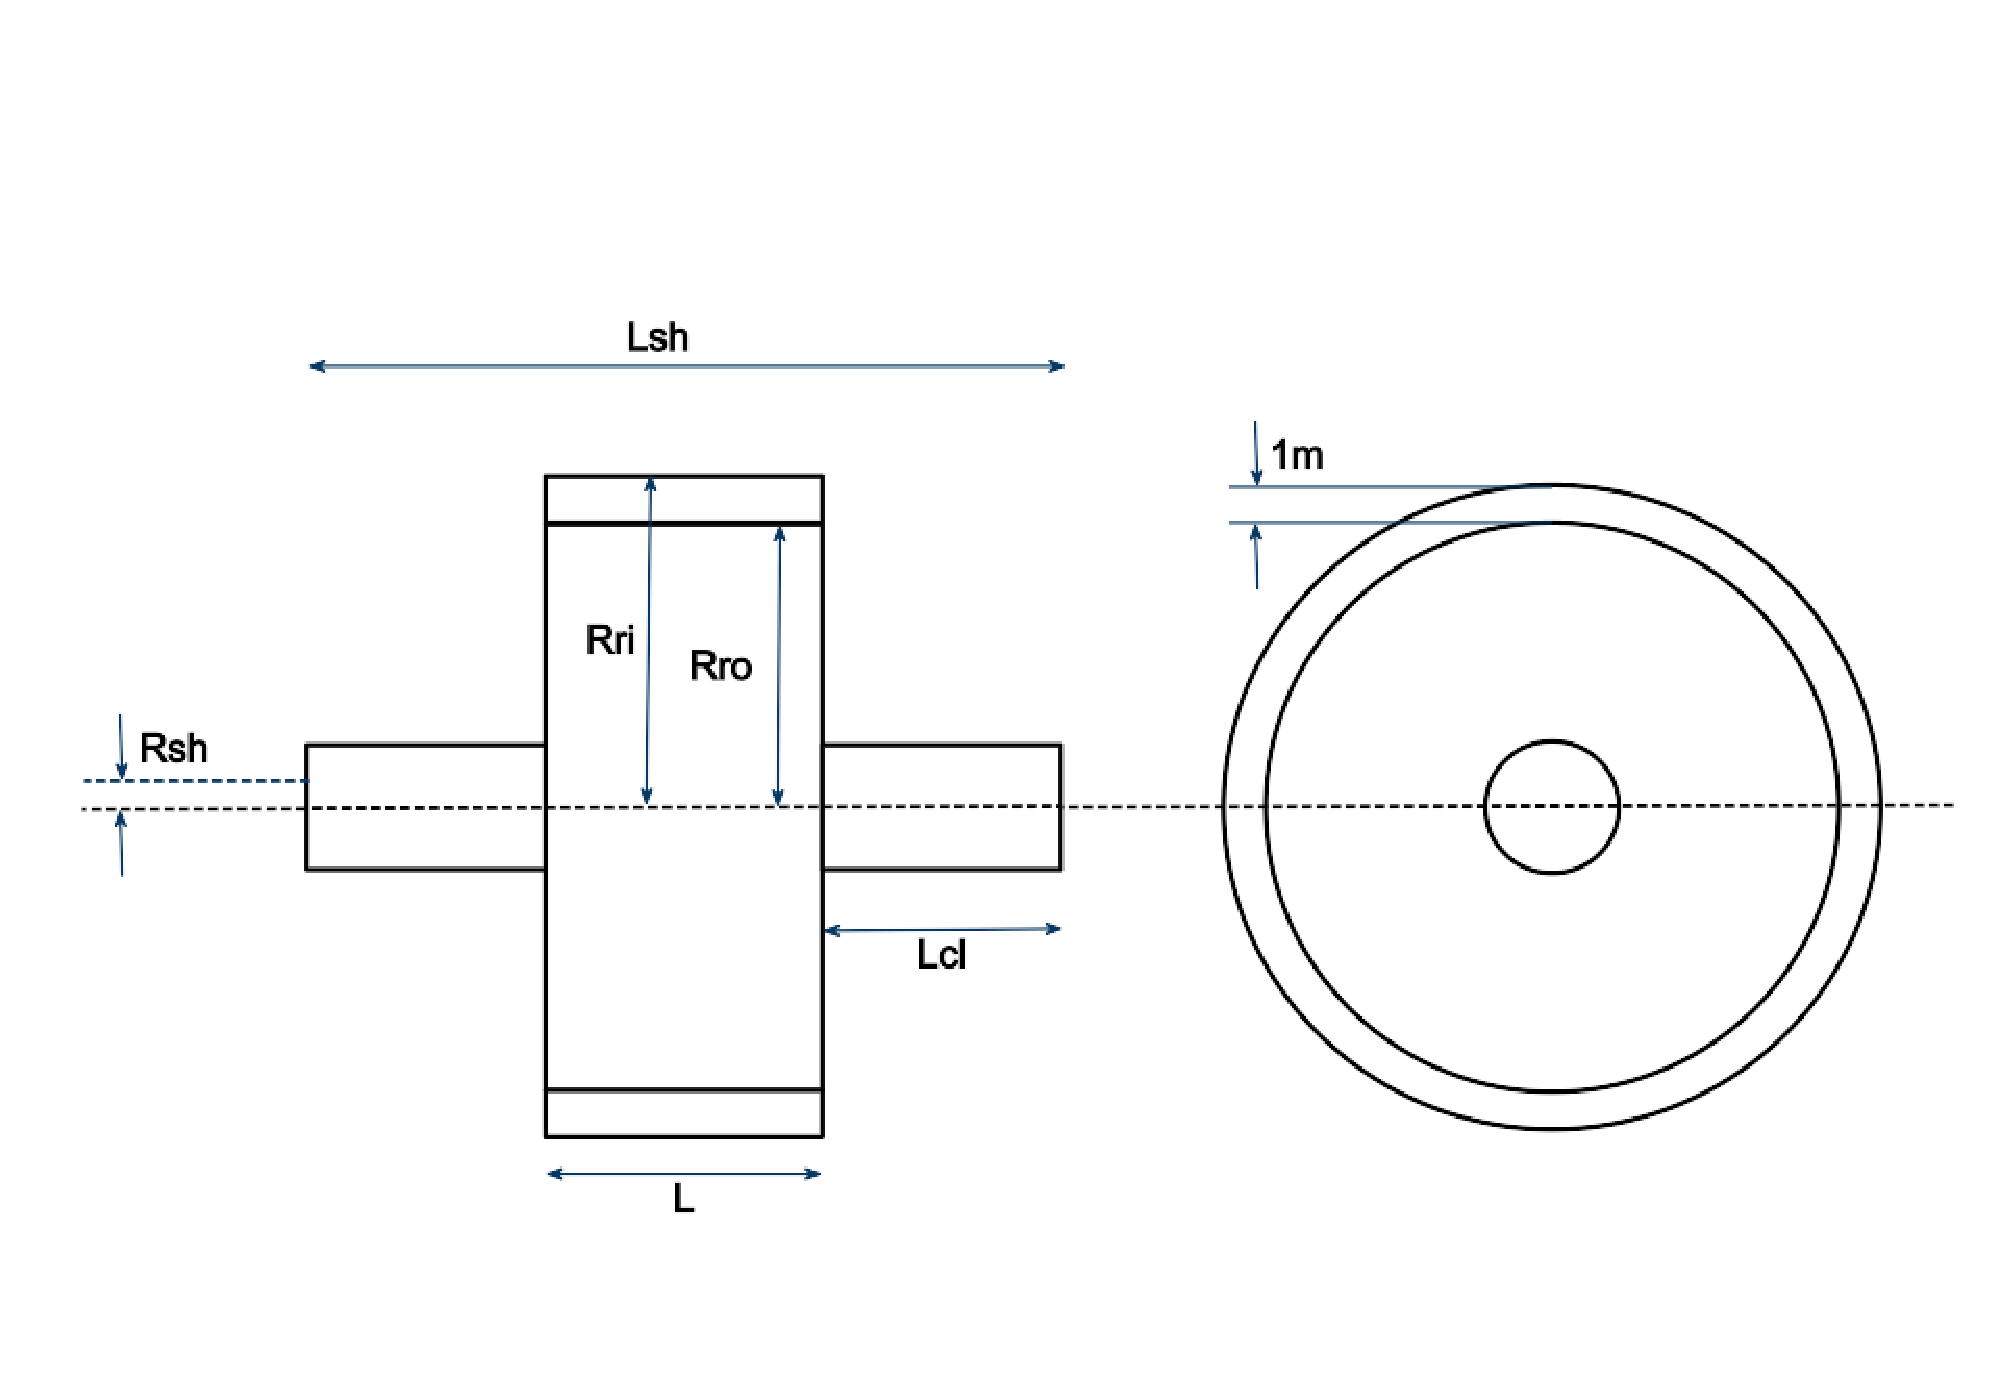
\includegraphics[width=46mm, height=33mm] {diagrams/bdcpmRotor.eps}
        \label{pcaEVbdcpmAll.eps}
      }
      \label{bdcpmvars}
    \end{center}
  \end{figure}



 %  \frametitle{Schematics of BDCPM motor}
 %  \begin{figure}[ht]\begin{center}
 %      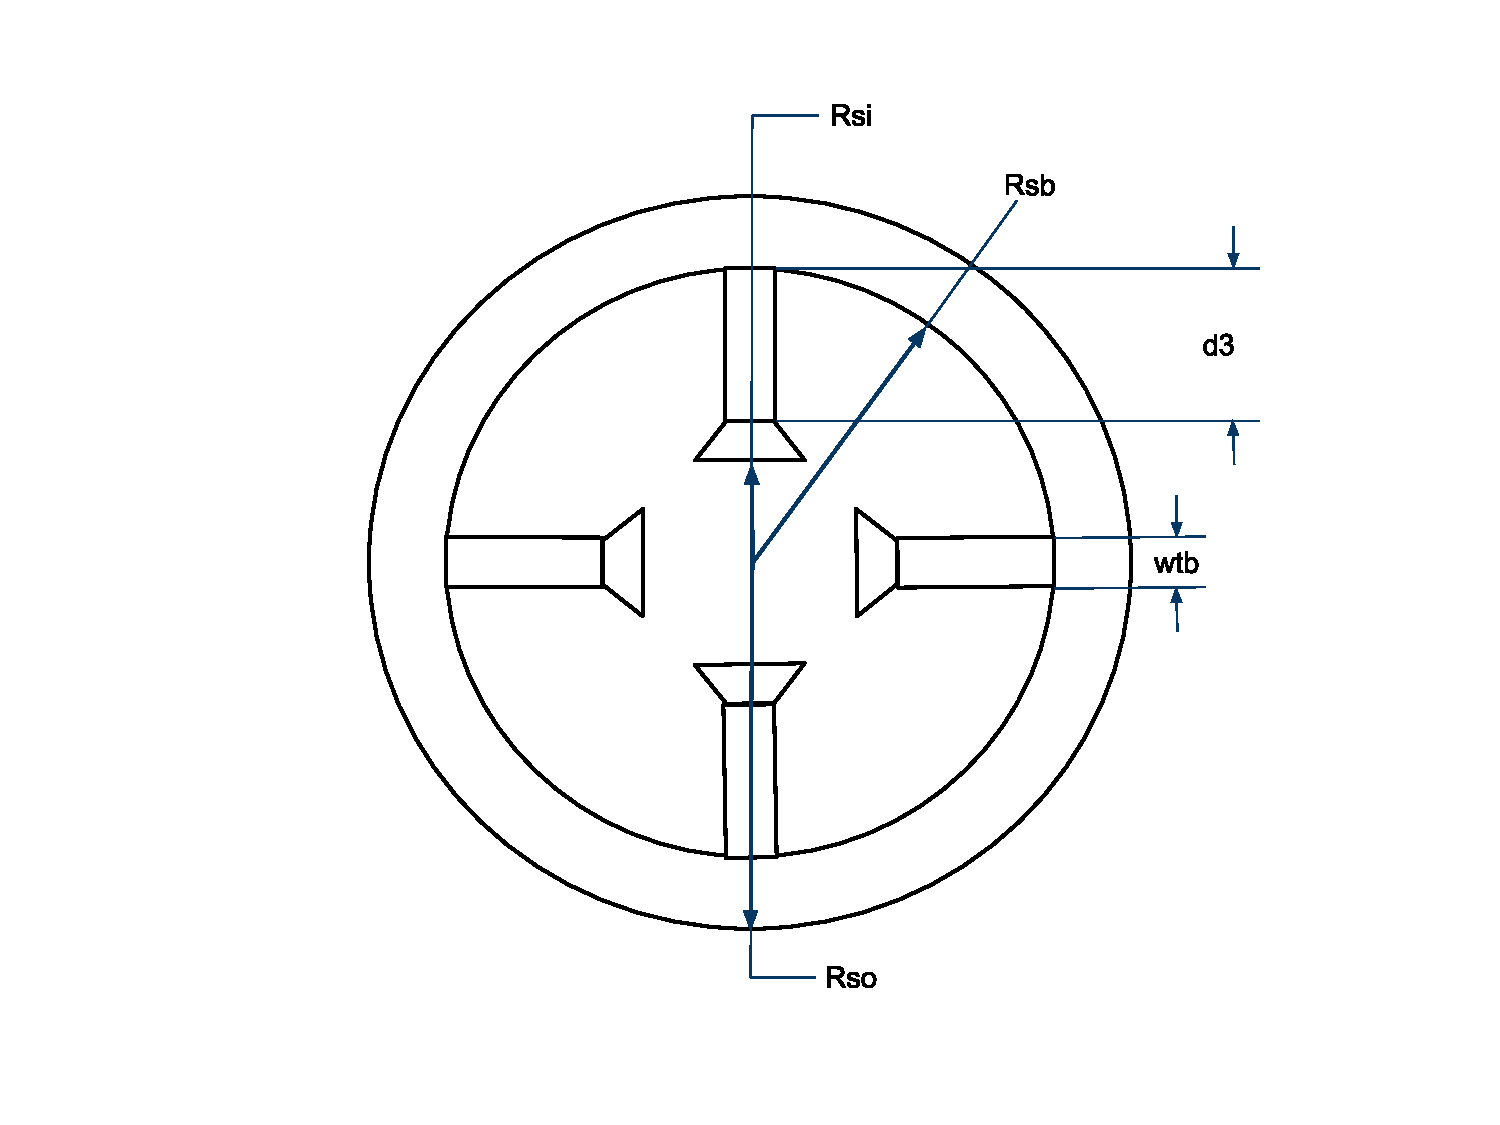
\includegraphics[width=35mm, height=28mm]{diagrams/bdcpmStator.eps}
 %      \caption{BDCPMM Stator assembly.}
 %      \label{bdcpmStator}
 %    \end{center}
 %  \end{figure}
 
 % \begin{figure}[ht]
 %    \begin{center}
 %      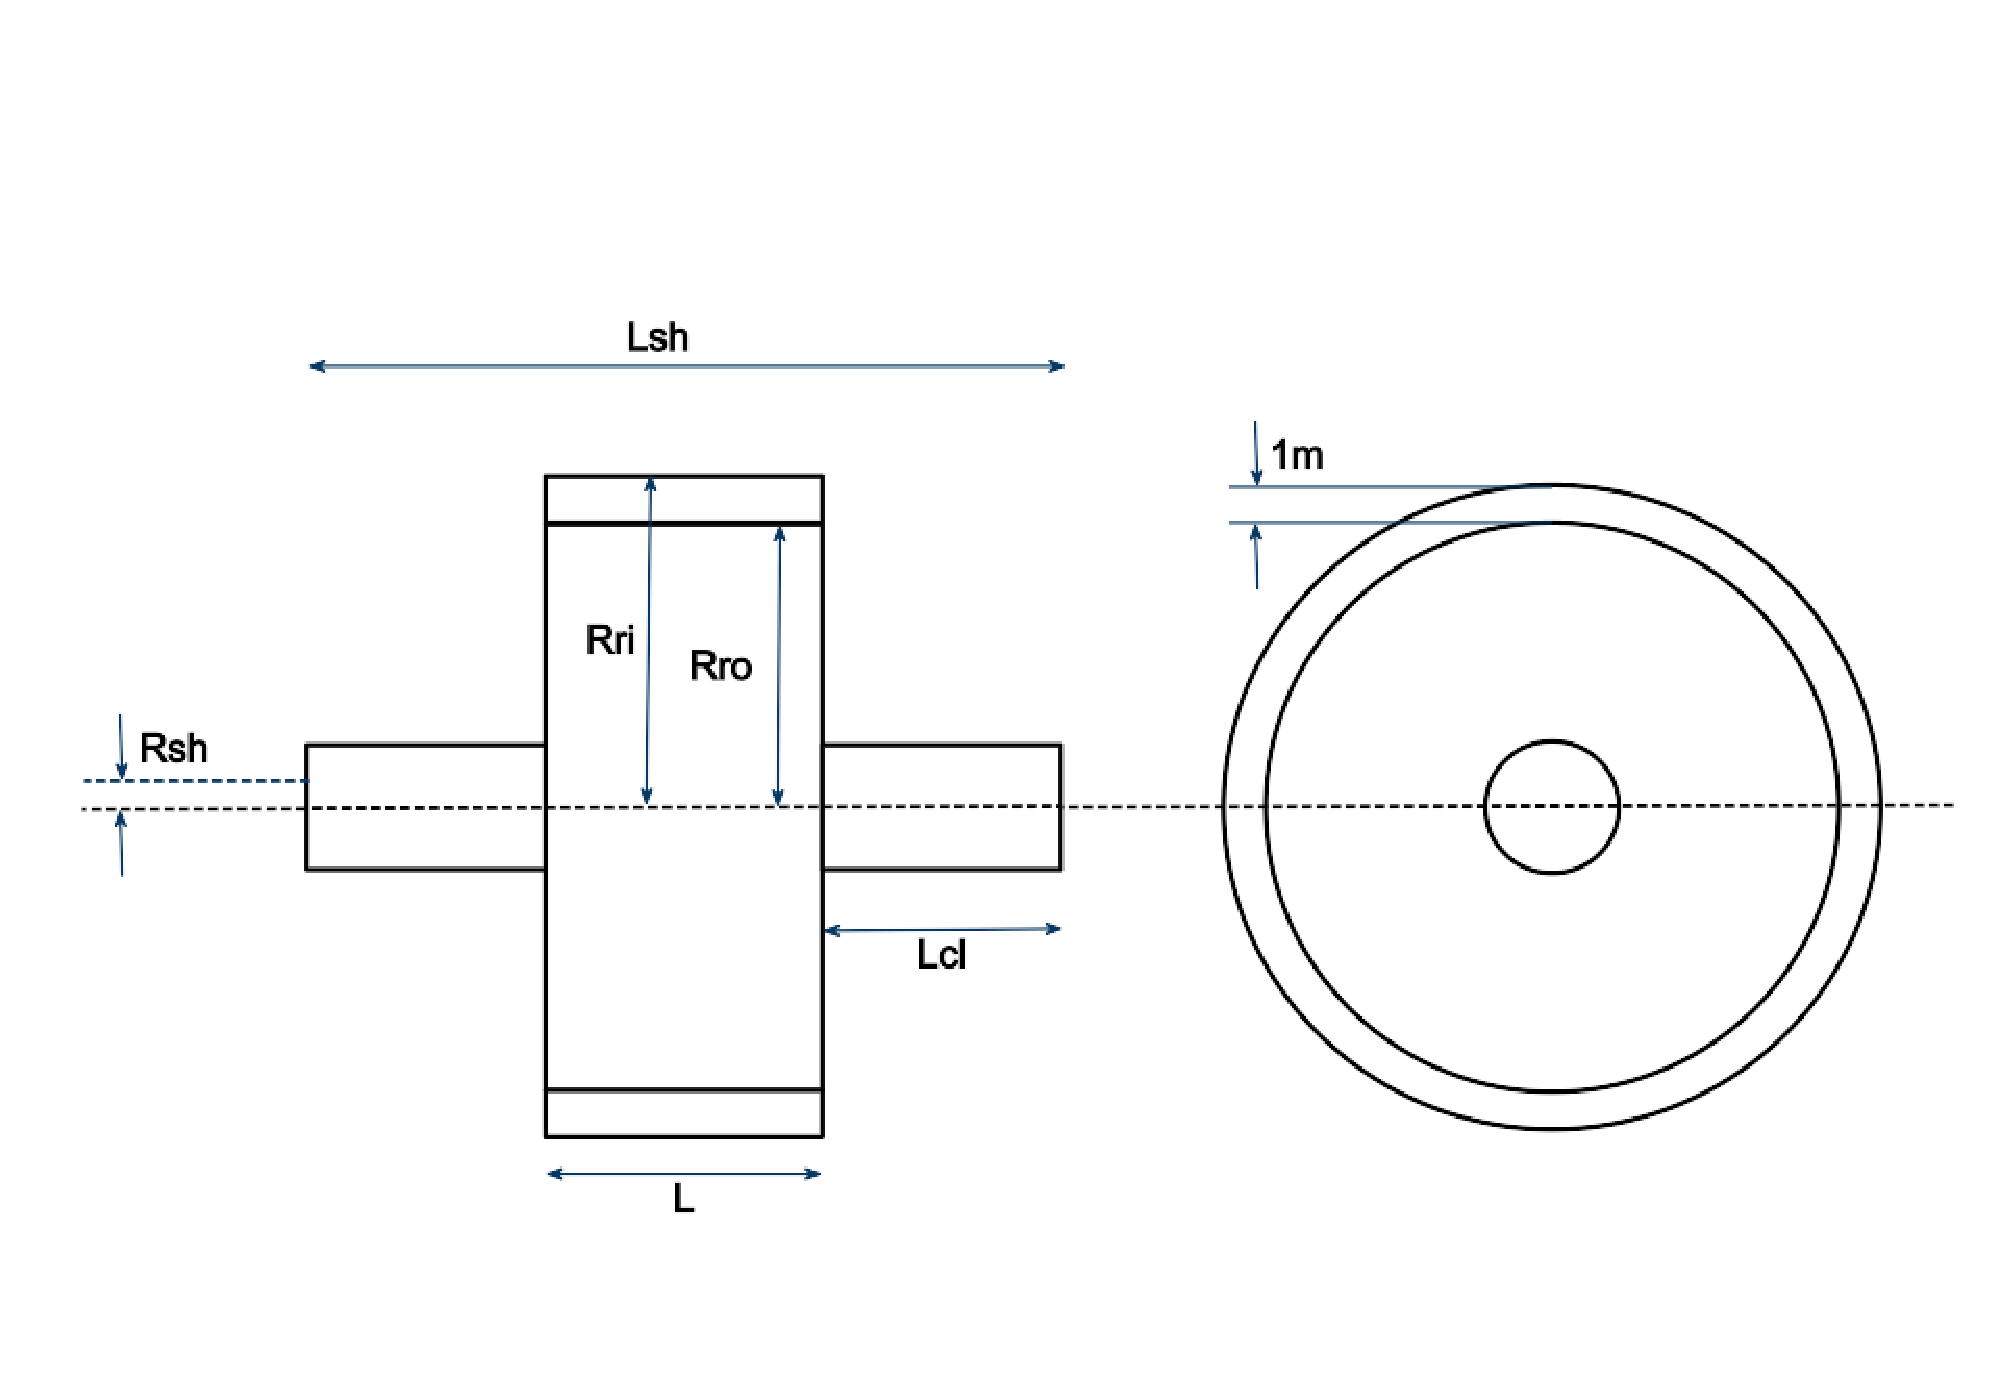
\includegraphics[width=40mm, height=28mm]{diagrams/bdcpmRotor.eps}
 %      \caption{BDCPMM Rotor Assembly.}
 %      \label{bdcpmRotor}
 %    \end{center}
 %  \end{figure}
\end{frame}


\begin{frame}
  \frametitle{Pareto front for the BDCPMM design problem}
  \begin{figure}[ht]\begin{center}
      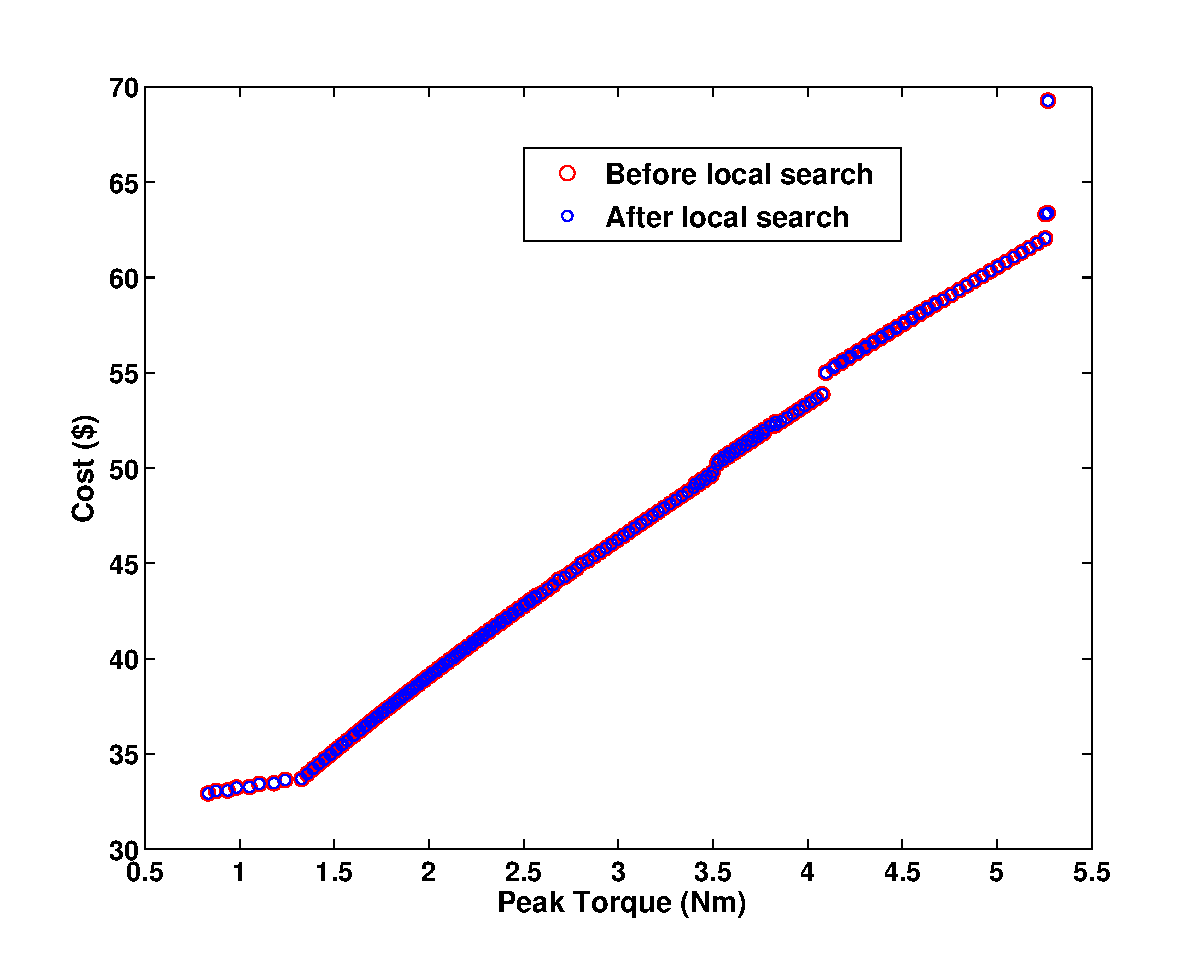
\includegraphics[width=65mm, height=55mm]{diagrams/nsplsp.eps} 
      \label{nsplsp}
    \end{center}
  \end{figure}
\end{frame}

\begin{frame}
  \frametitle{Isomap and PCA results for the pareto-front}
  
  \begin{figure}[ht]
    \begin{center}
      \subfigure[Isomap residual variance] {
        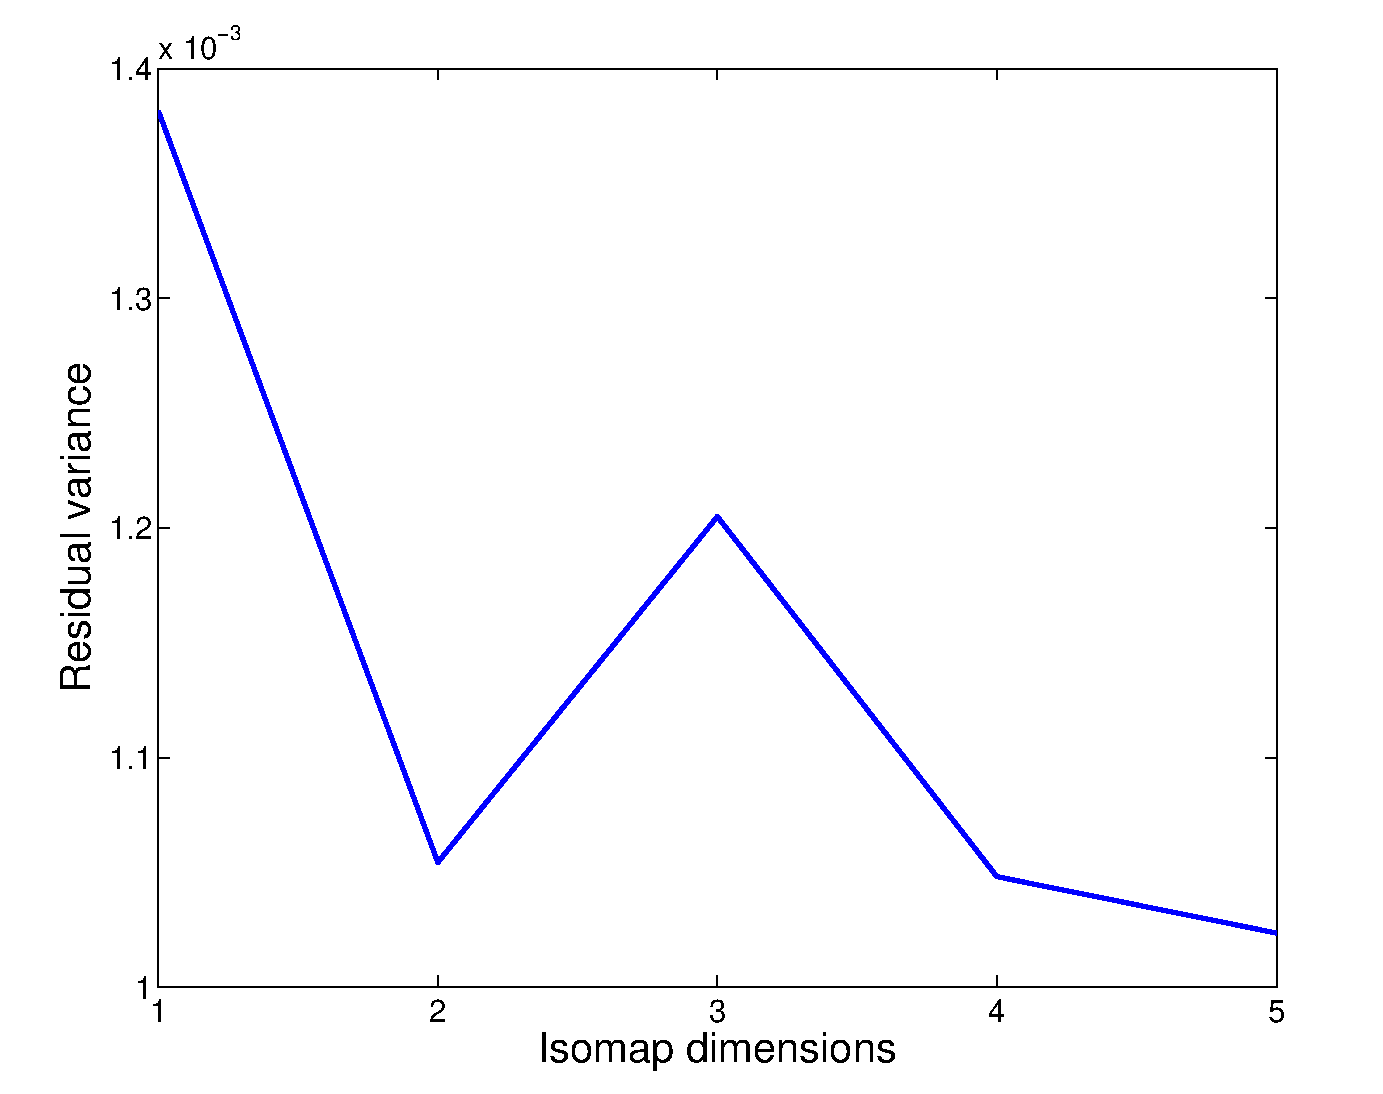
\includegraphics[width=38mm, height=30mm] {diagrams/isoRVbdcpmAll.eps}
        \label{isoRVbdcpmAll}
      }
      \subfigure[PCA explained variance] {
        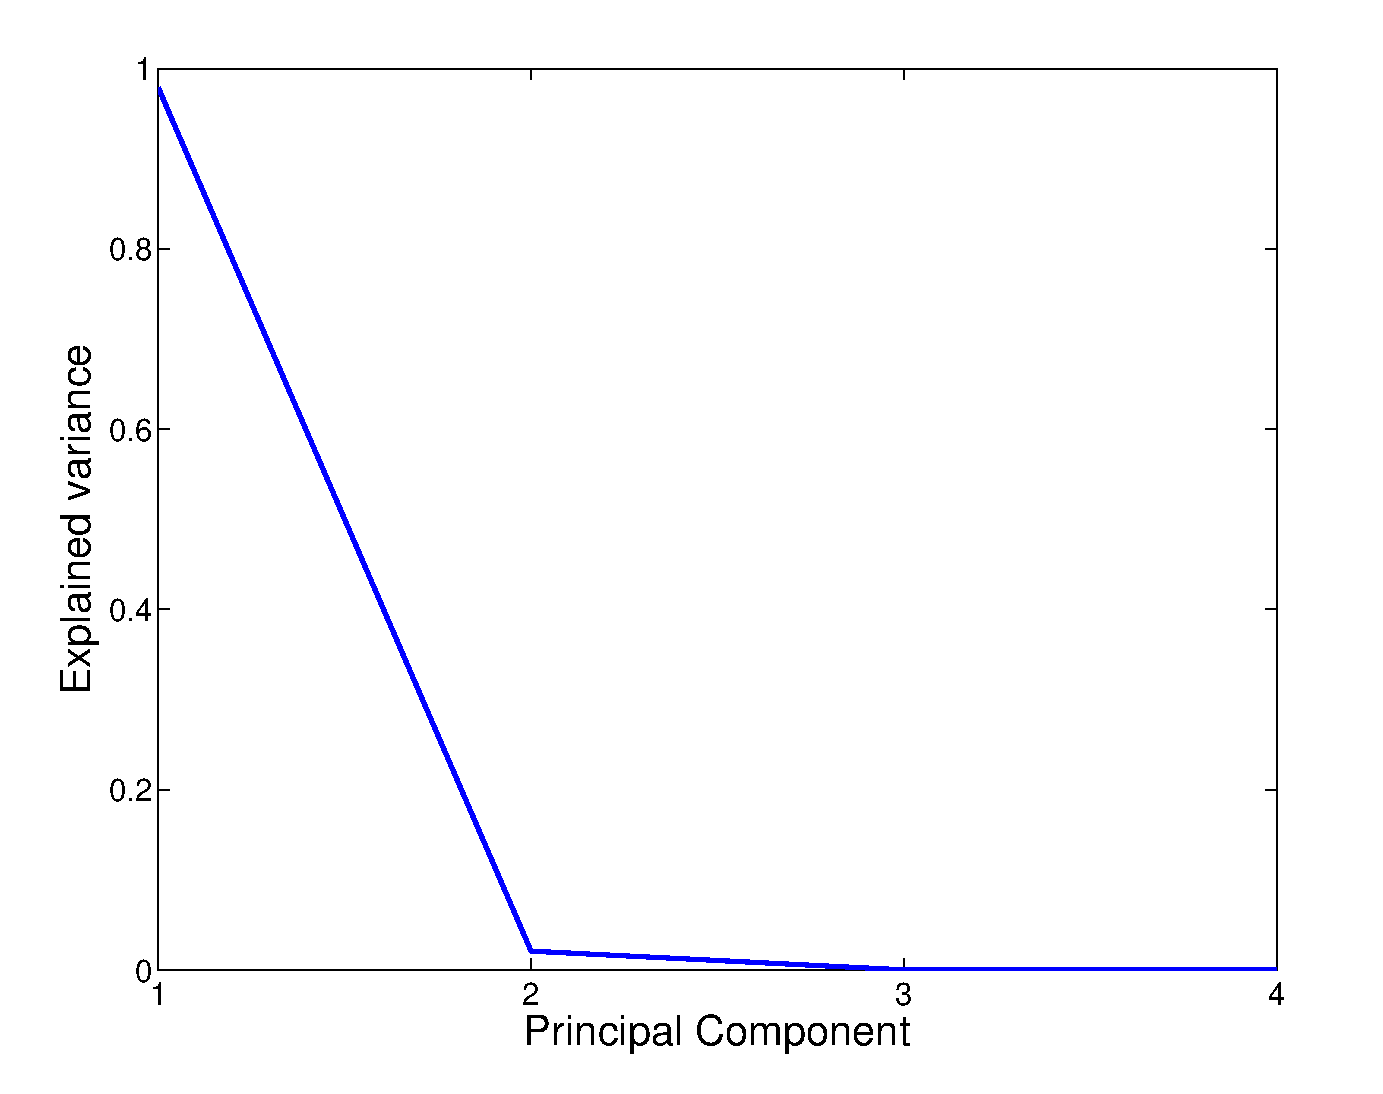
\includegraphics[width=38mm, height=30mm] {diagrams/pcaEVbdcpmAll.eps}
        \label{pcaEVbdcpmAll.eps}
      }
      \label{bdcpmvars}
    \end{center}
  \end{figure}

  {\small
    \begin{table}[!ht]
      \centering
      \begin{tabular}{c|c|c|c|c|c|}
        \cline{2-6}
        & $n_l$ & $N$ & $ L_{type} $  & $ M_{ph}$ & $a_{gauge}$ \\
        \hline
        \multicolumn{1}{|c|}{First PC} & 0.9993 & 0.0370 & 0.0072 & 0 & -0.0024\\
        \hline
        \multicolumn{1}{|c|}{Second PC} & -0.0367 & 0.9943 & 0.0165 & 0 & 0.0985\\
        \hline
      \end{tabular}
      \caption{First two principal components of the BDCPM data.}
      \label{first2BDPCs}
    \end{table}
  }



 %     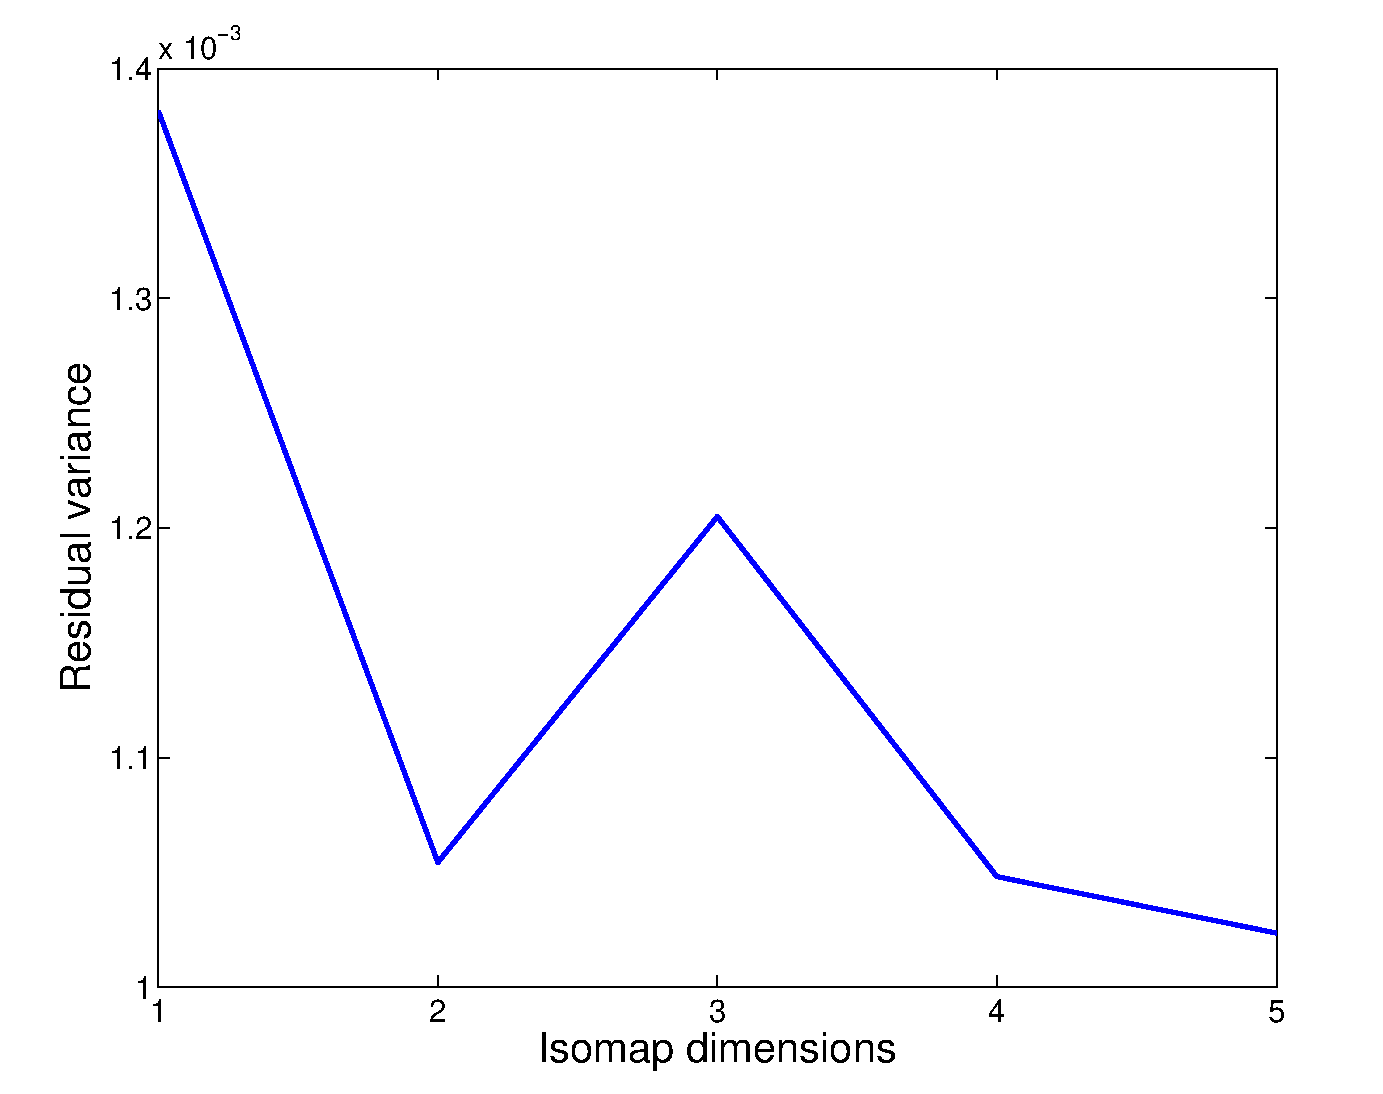
\includegraphics[width=30mm, height=25mm]{diagrams/isoRVbdcpmAll.eps}
  %     \caption{Isomap residual variance for BDCPMM design problem pareto-front.}
  %     \label{isoRVbdcpmAll}
  %   \end{center}
  % \end{figure}
 
  % \begin{figure}[ht]
  %   \begin{center}
  %     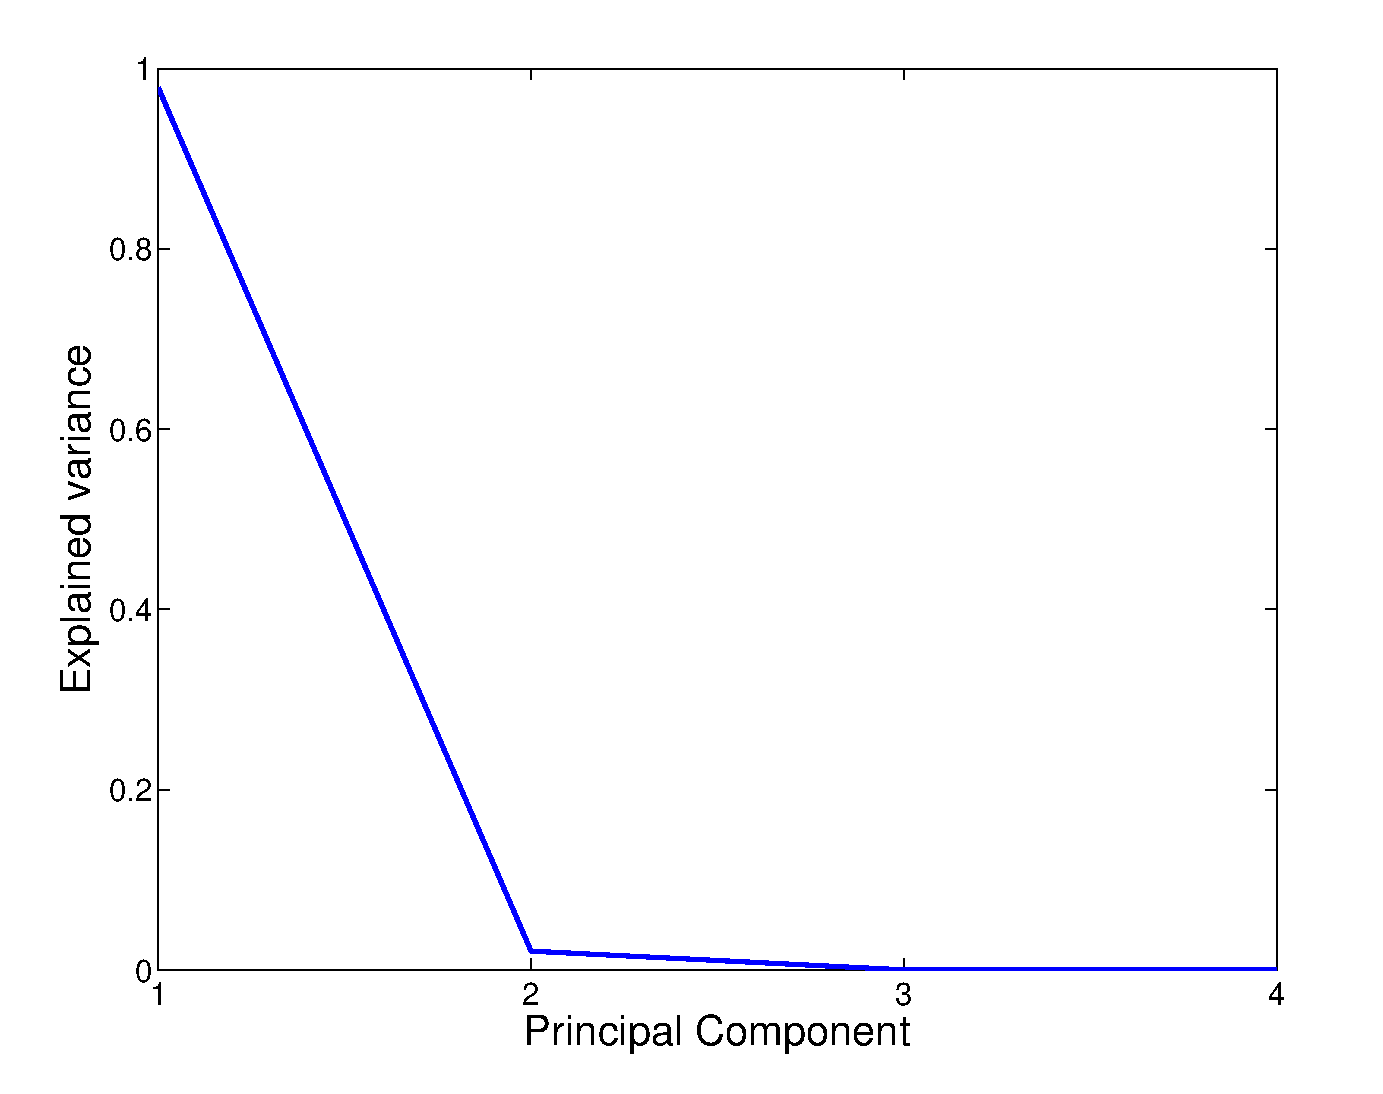
\includegraphics[width=30mm, height=25mm]{diagrams/pcaEVbdcpmAll.eps}
  %     \caption{PCA explained variances for BDCPMM design problem pareto-front.}
  %     \label{pcaEVbdcpmAll}
  %   \end{center}
  % \end{figure}

\end{frame}




\begin{frame}

  \frametitle{Clusters in the BDCPMM pareto-front}  
  \begin{figure}[ht]
    \begin{center}
      \subfigure[Clusters as seen in the objective space.] {
        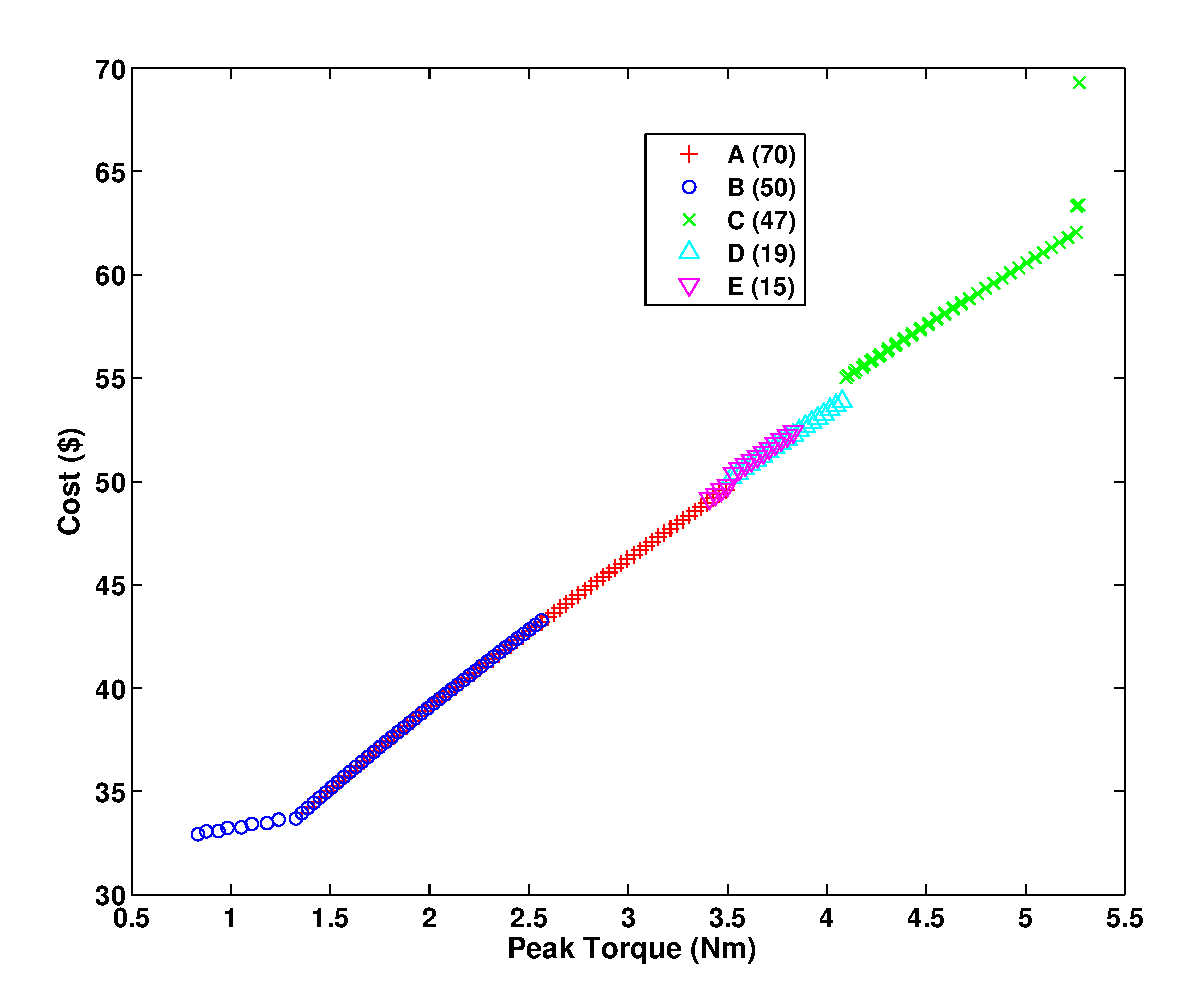
\includegraphics[width=40mm, height=35mm] {diagrams/bClustersO3.eps}
        \label{isoRVbdcpmAll}
      }
      \subfigure[Clusters as seen in the decision space.] {
        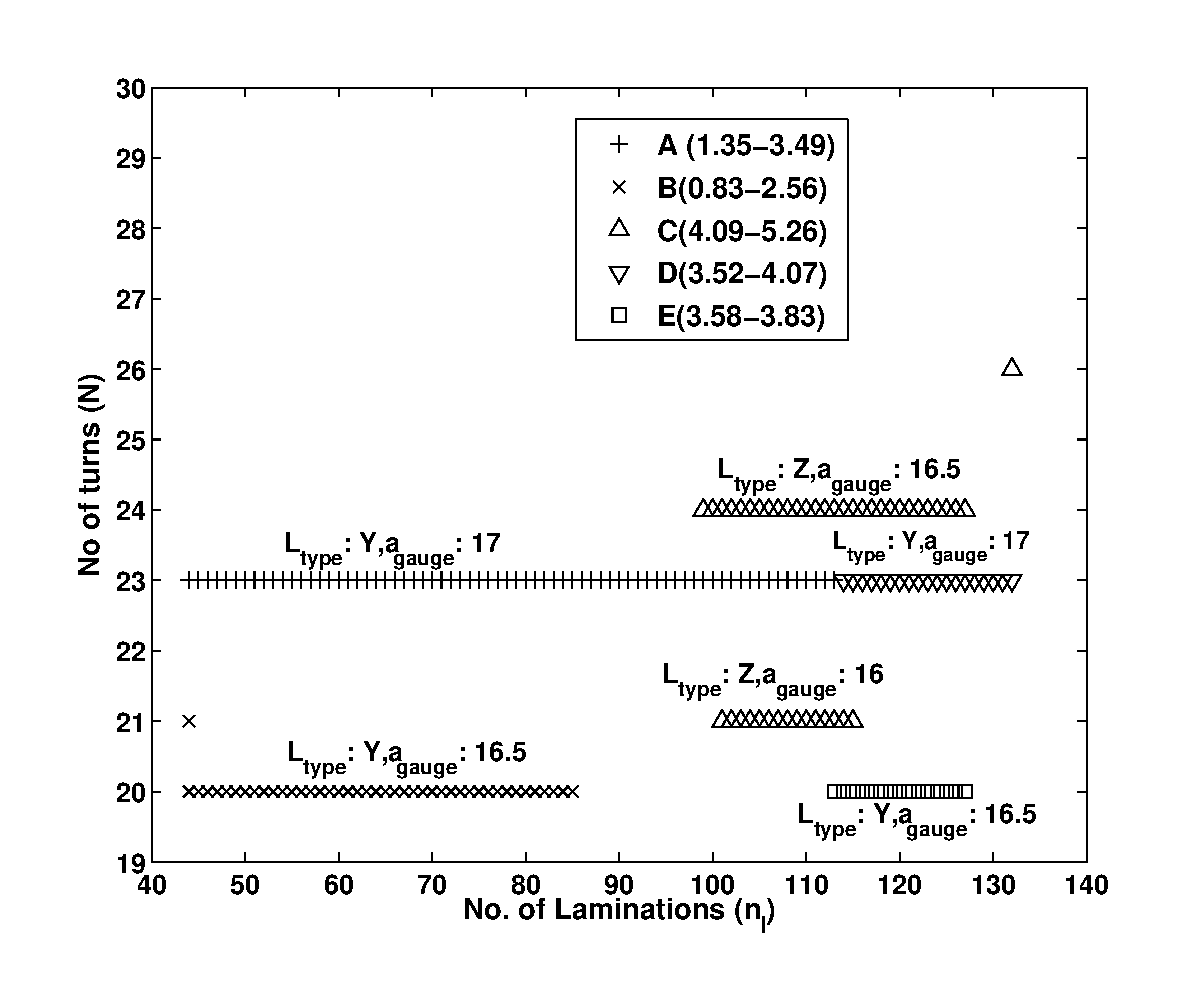
\includegraphics[width=40mm, height=35mm] {diagrams/bclustersp3.eps}
        \label{pcaEVbdcpmAll.eps}
      }
      \label{bdcpmvars}
    \end{center}
  \end{figure}


\end{frame}





\begin{frame}

  \frametitle{Isomap and PCA analysis of the clusters.}  
  \begin{itemize}
  \item Four of the clusters are one dimensional manifolds.
  \item Both Isomap and PCA variances show cluster \textbf{C} with two
    dimensions.
  \end{itemize}


  \begin{figure}[ht]
    \begin{center}
      \subfigure[Residual variance for the cluster C] {
        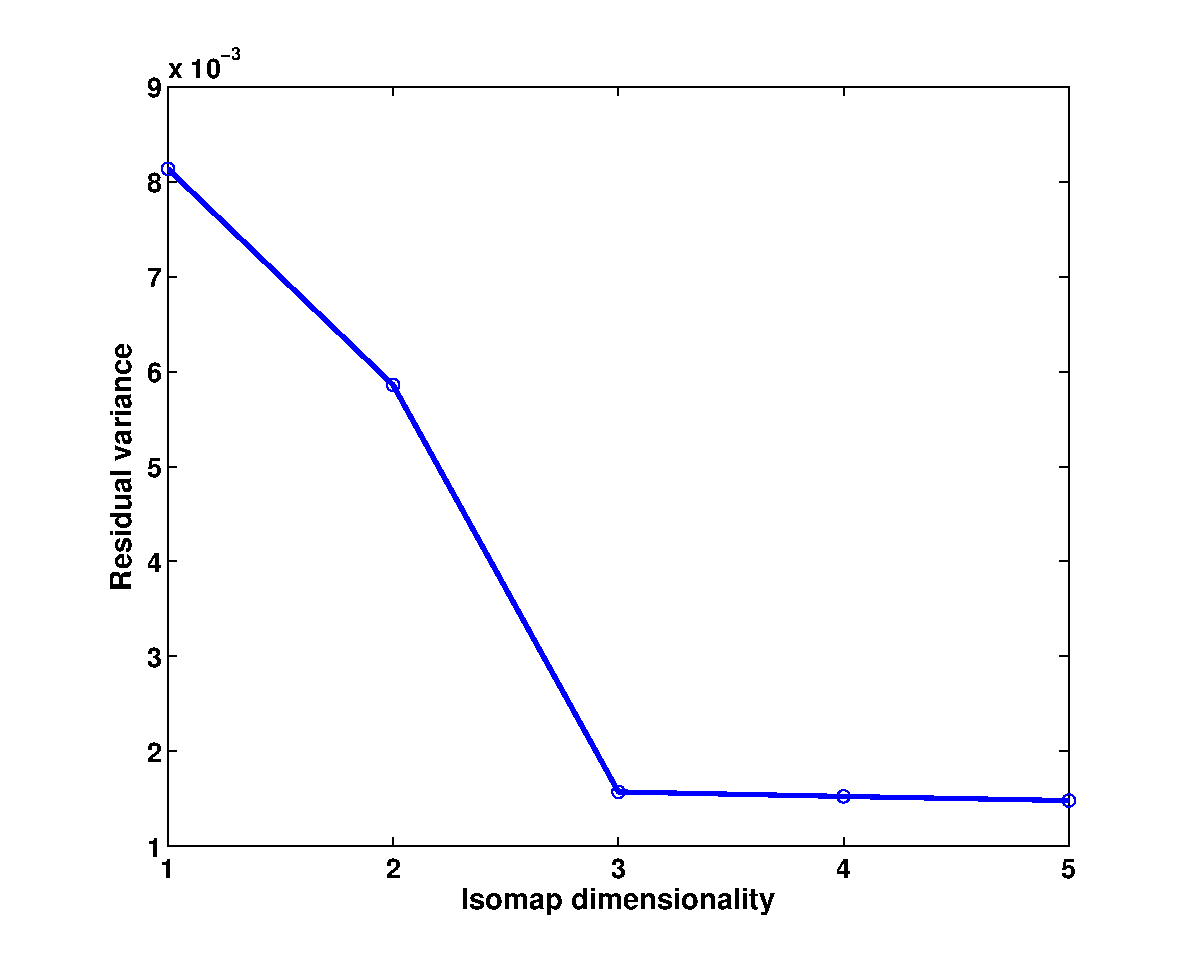
\includegraphics[width=40mm, height=35mm] {diagrams/bclusterCrv.eps}
        \label{bdcpmclrv}
      }
      \subfigure[Explained variance for the clusters.] {
        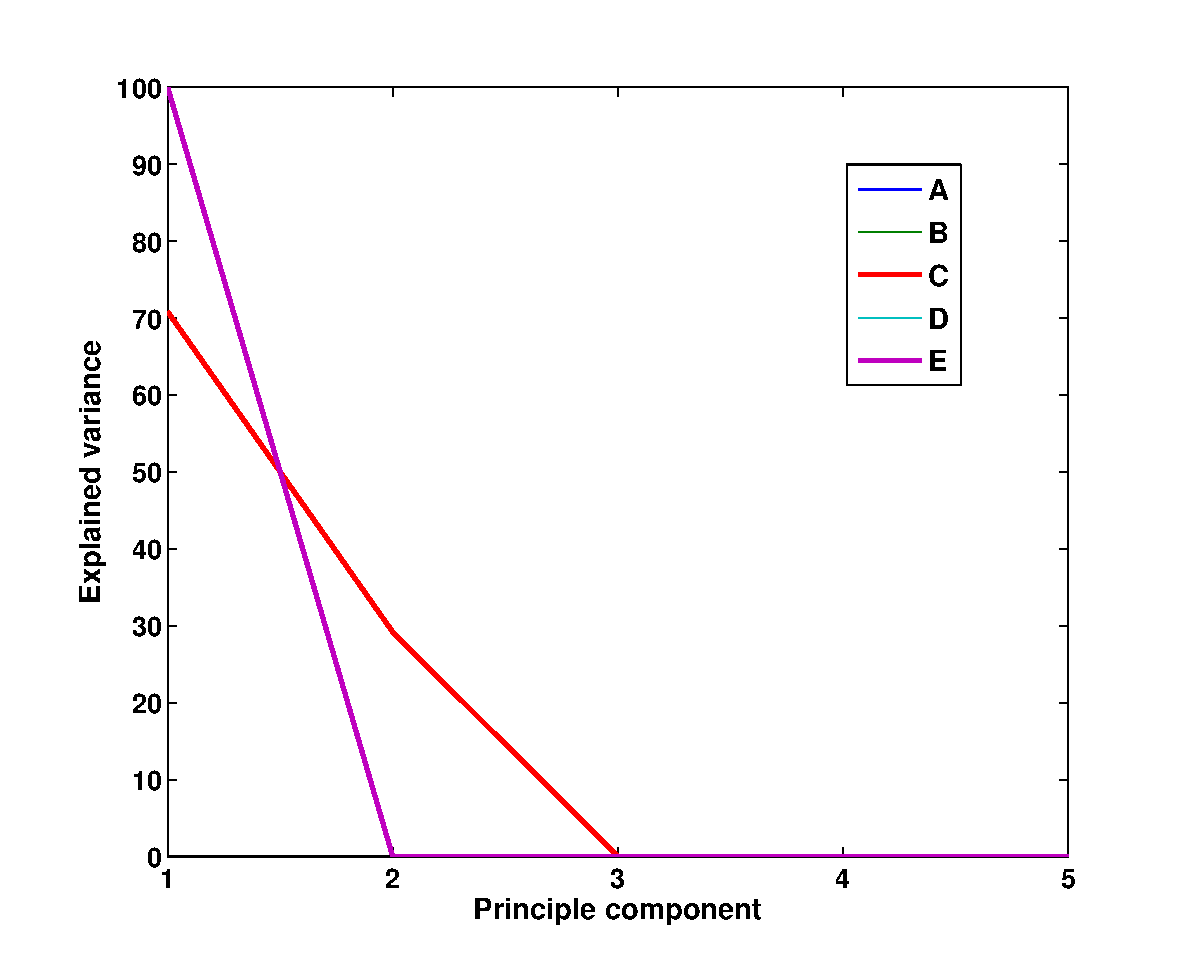
\includegraphics[width=40mm, height=35mm] {dia/bdcpmClustersEV.eps}
        \label{bdcpmclev}
      }
      \label{bdcpmvars}
    \end{center}
  \end{figure}


\end{frame}  

%   % \frametitle{Isomap residual variance for the cluster \textbf{C}}
%   % \begin{figure}[ht]
%   %   \begin{center}
%   %     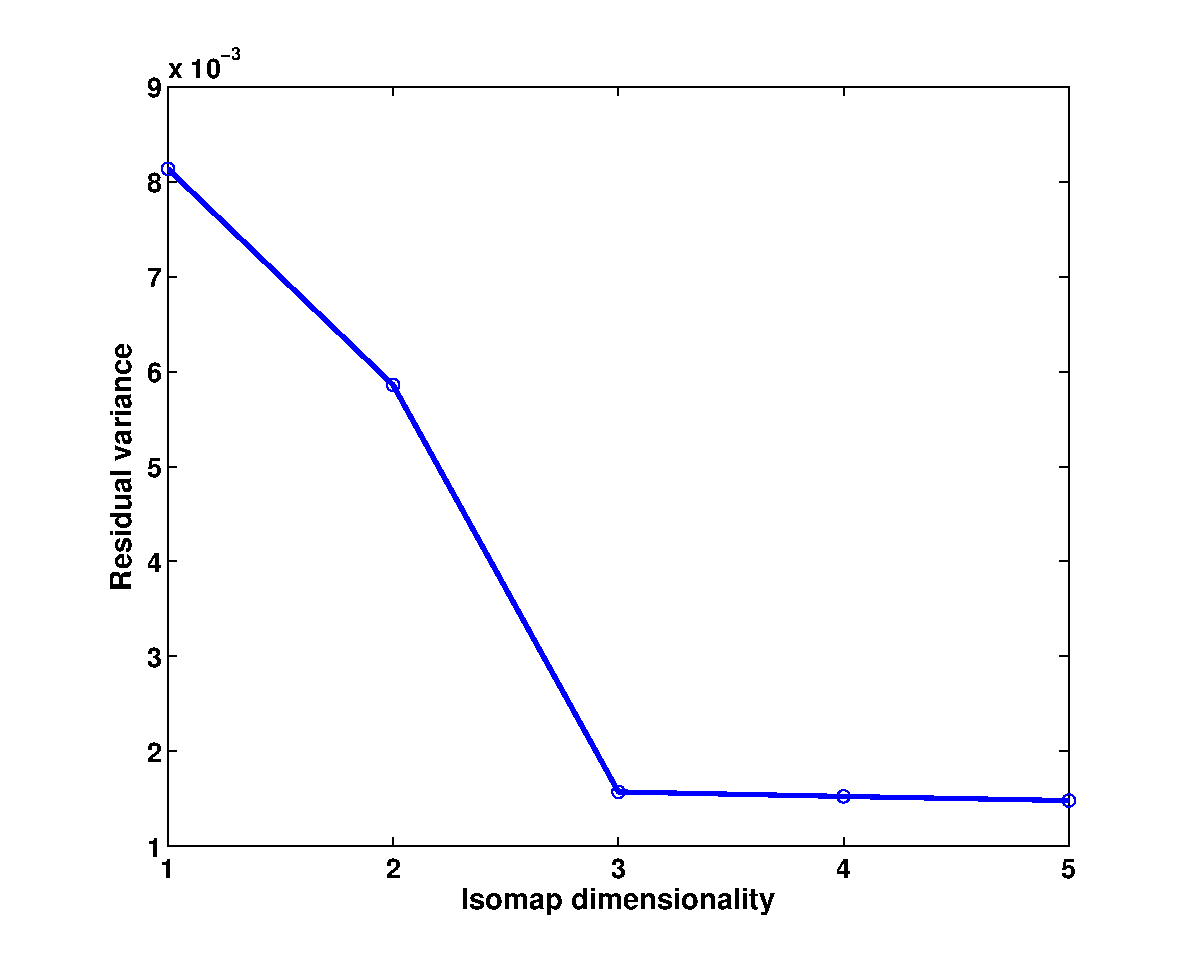
\includegraphics[width=60mm, height=50mm]{diagrams/bclusterCrv.eps} 
%   %     \caption{Residual variance for the cluster \textbf{C}.}
%   %     \label{bClusterCrv}
%   %   \end{center}
%   % \end{figure}



\begin{frame}
  \frametitle{Principal components of the clusters}
  \begin{itemize}
  \item All the one dimensional clusters are lines parallel to the $n_l$ dimension
  \item Cluster \textbf{C} is embedded in the $n_l-N$ plane.
  \end{itemize}

  \begin{table}[!ht]
    \centering
    \begin{tabular}{c|c|c|c|c|c|}
      
      \cline{2-6}
      & $n_l$ & $N$ & $ L_{type} $  & $ M_{ph}$ & $a_{gauge}$ \\
      \hline
      \multicolumn{1}{|c|}{\textbf{A}} & 1 & 0 & 0 & 0 & 0 \\
      \hline
      \multicolumn{1}{|c|}{\textbf{B}} & 0.999 & 0.0077 & 0 & 0 & -0.019\\
      \hline
      \multicolumn{1}{|c|}{\multirow{2}{*}{\textbf{C}}} & 0.789 & 0.610 & 0 & 0 & 0.066\\ \cline{2-6}
      \multicolumn{1}{|c|}{}& -0.613 & 0.785 & 0 & 0 & 0.074\\
      \hline
      \multicolumn{1}{|c|}{\textbf{D}} & 1 & 0 & 0 & 0 & 0\\
      \hline
      \multicolumn{1}{|c|}{\textbf{E}} & 1 & 0 & 0 & 0 & 0\\
      \hline
    \end{tabular}
    \label{clusterPC}
  \end{table}
\end{frame}


\begin{frame}
  \frametitle{Design implications}
  
  \begin{itemize}
    \item $Y$ connection should be used in BDCPM designs.
    \item For low torque motors, laminations with low radial dimensions
      should be used.
    \item Thicker wires and small number of turns in the stator coil should
      be used.
    \item For high torque motors, laminations with large radial dimension
      and thick wires for stator winding should be used.
    
  \end{itemize}

\end{frame}




\subsection{B. Gearbox design problem}

\begin{frame}
  \frametitle{Gearbox design problem}
  \begin{figure}[ht]\begin{center}
      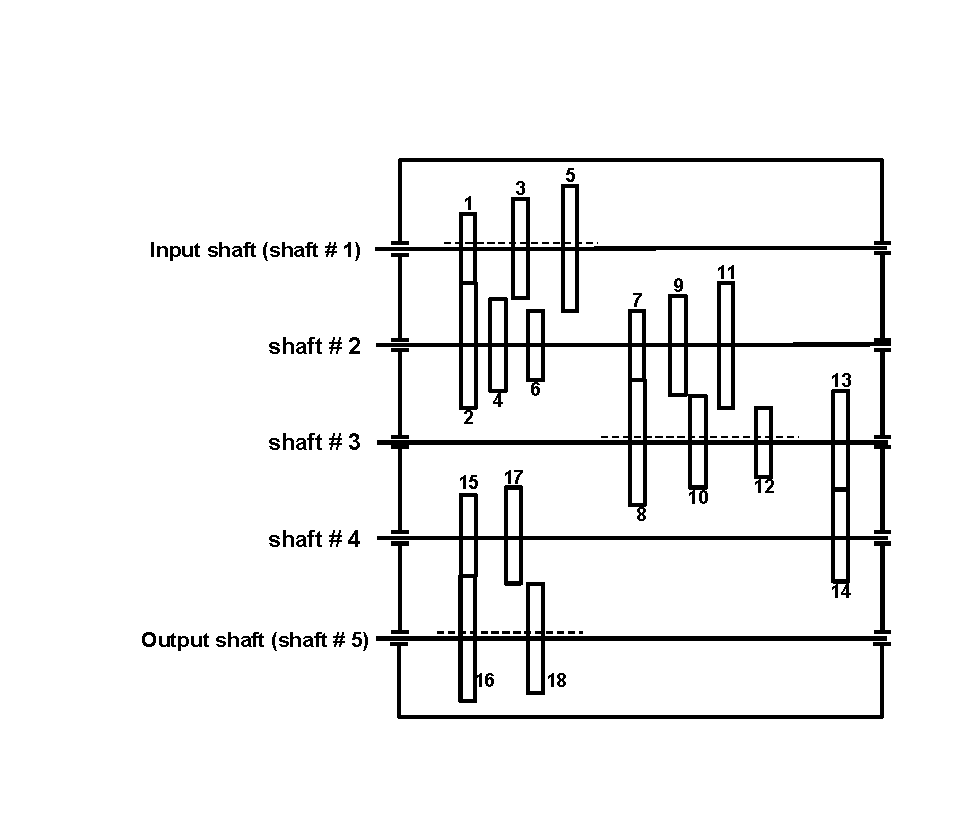
\includegraphics[width=75mm, height=60mm]{diagrams/geartrain.eps}
      \caption{18-speed Gearbox schematics.}
      \label{geartrain}
    \end{center}
  \end{figure}

\end{frame}


\begin{frame}[allowframebreaks]
  \frametitle{Optimization problem}
  \begin{itemize}
  \item Two instances of the problem:
    \begin{enumerate}[(A)]
    \item Fixed gear-teeth layout 11 variable problem in which power and
      minimization of gearbox weight are the objectives.
    \item 29 variable problem with three objectives.
    \end{enumerate}

  \end{itemize}

  
\end{frame}



\begin{frame}
  \frametitle{Pareto-front for the fixed gear ratio problem}

  \begin{itemize}
  \item 927 points in the pareto-front.
  \item 11 clusters are obtained in the clustering.
  \end{itemize}

  \begin{figure}[ht]\begin{center}
      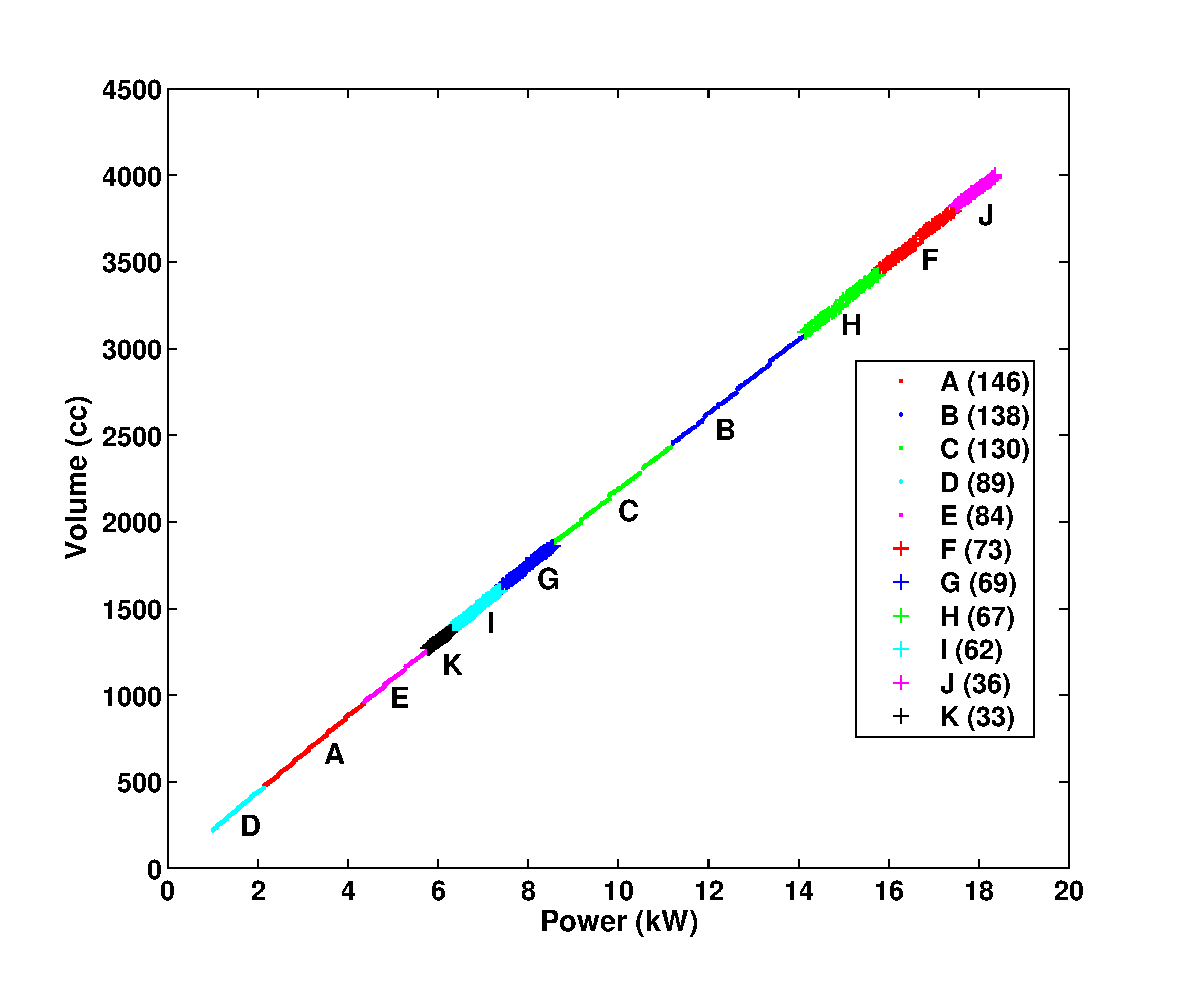
\includegraphics[width=65mm, height=50mm]{dia/gt11cpareto1.eps}
      \label{gt11Clusters}
    \end{center}
  \end{figure}
\end{frame}


\begin{frame}
  \frametitle{Isomap and PCA results for the pareto-front}

  \begin{itemize}
  \item Isomap residual variance shows a manifold dimensionality of four.
  \item PCA shows a linear dimensionality of one.
  \end{itemize}

  \begin{figure}[ht]
    \begin{center}
      \subfigure[Residual variance] {
        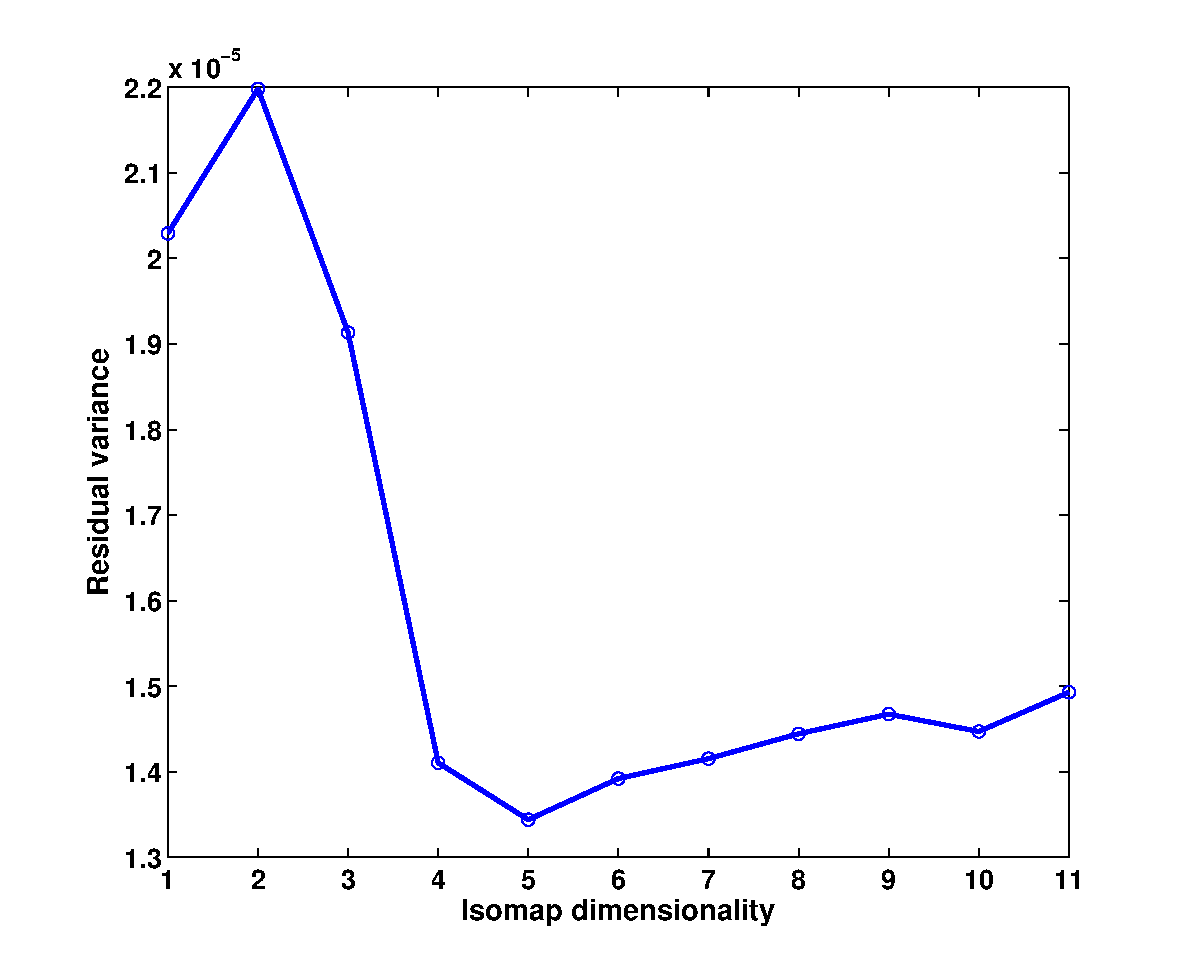
\includegraphics[width=40mm, height=35mm] {dia/gt11rv.eps}
        \label{gt11rv}
      }
      \subfigure[Explained variance.] {
        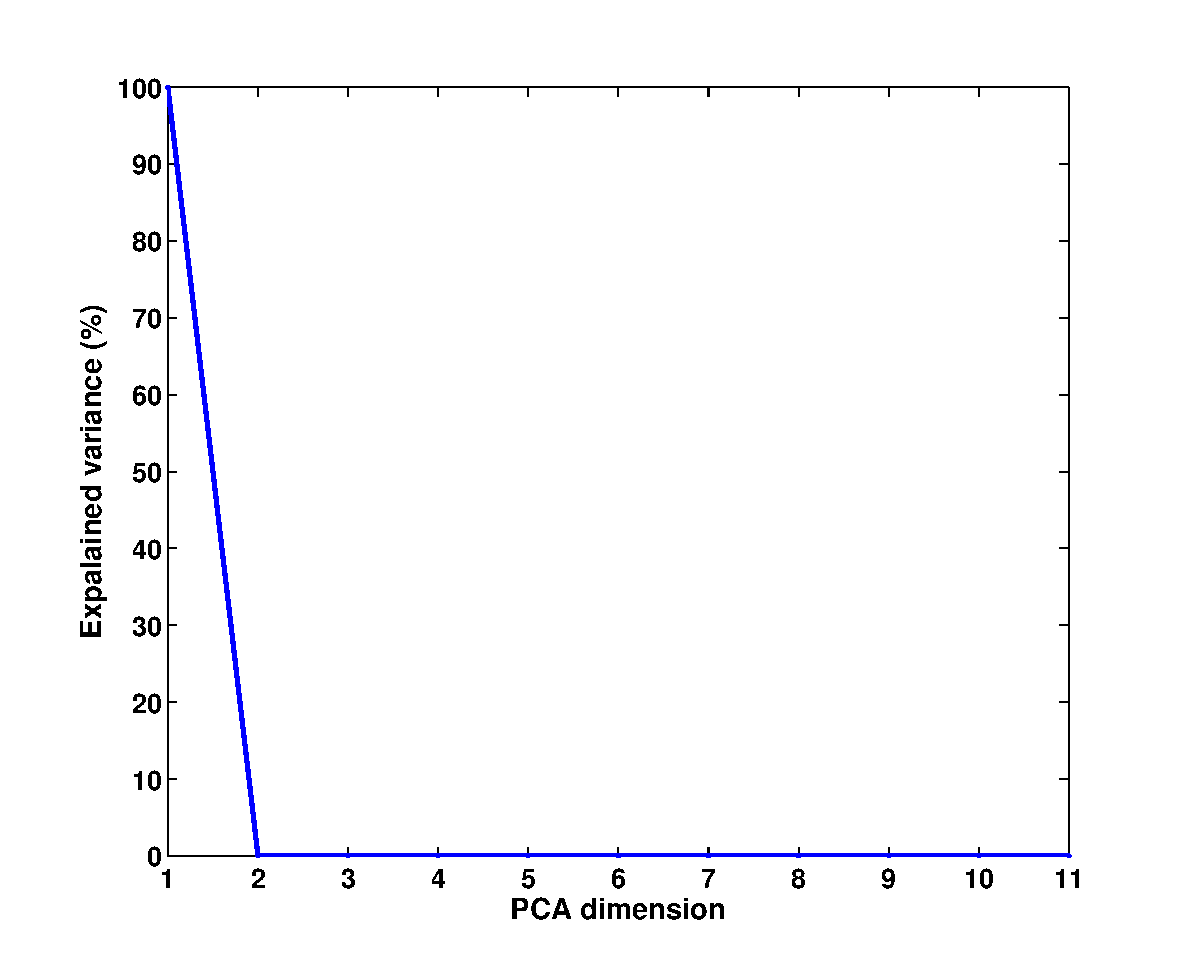
\includegraphics[width=40mm, height=35mm] {dia/gt11ev.eps}
        \label{gt11ev}
      }
      \label{gt11vars}
    \end{center}
  \end{figure}


\end{frame}


\begin{frame}
  \frametitle{Principal components of the pareto-front}

  \begin{itemize}
  \item Thickness of the gear-pairs in the final transmission stage are the
    most varying.
  \end{itemize}

  {\small
    \begin{table}[!ht]
      \centering
      \begin{tabular}{|c|c|c|c|c|c|}
        \hline
        \multirow{2}{*}{First PC}   & ($t_9$) &  ($t_8$) &  ($t_7$)  & ($t_6$) & ($p$)\\
        & -0.8444  & -0.4617  & 0.1837 & -0.1511 & 0.0733  \\
        \hline
        \multirow{2}{*}{Second PC}   & ($m$) &  ($t_5$) &  ($t_6$)  & ($t_9$) & ($t_8$)\\
        & 0.9997 & -0.0124 & 0.0097 & 0.0087 &  0.0087 \\
        \hline
      \end{tabular}
      \label{first2GT11PCs}
    \end{table}
  }

\end{frame}



\begin{frame}

  \begin{itemize}
  \item Most clusters have negligible residual variances.
  \item Residual variance for the cluster D shows a manifold dimension of one.
  \item PCA explained variance shows two significant principal components
    for cluster D.
  \end{itemize}

  \frametitle{Isomap and PCA results for the clusters}

  \begin{figure}[ht]
    \begin{center}
      \subfigure[Residual variance for the cluster D] {
        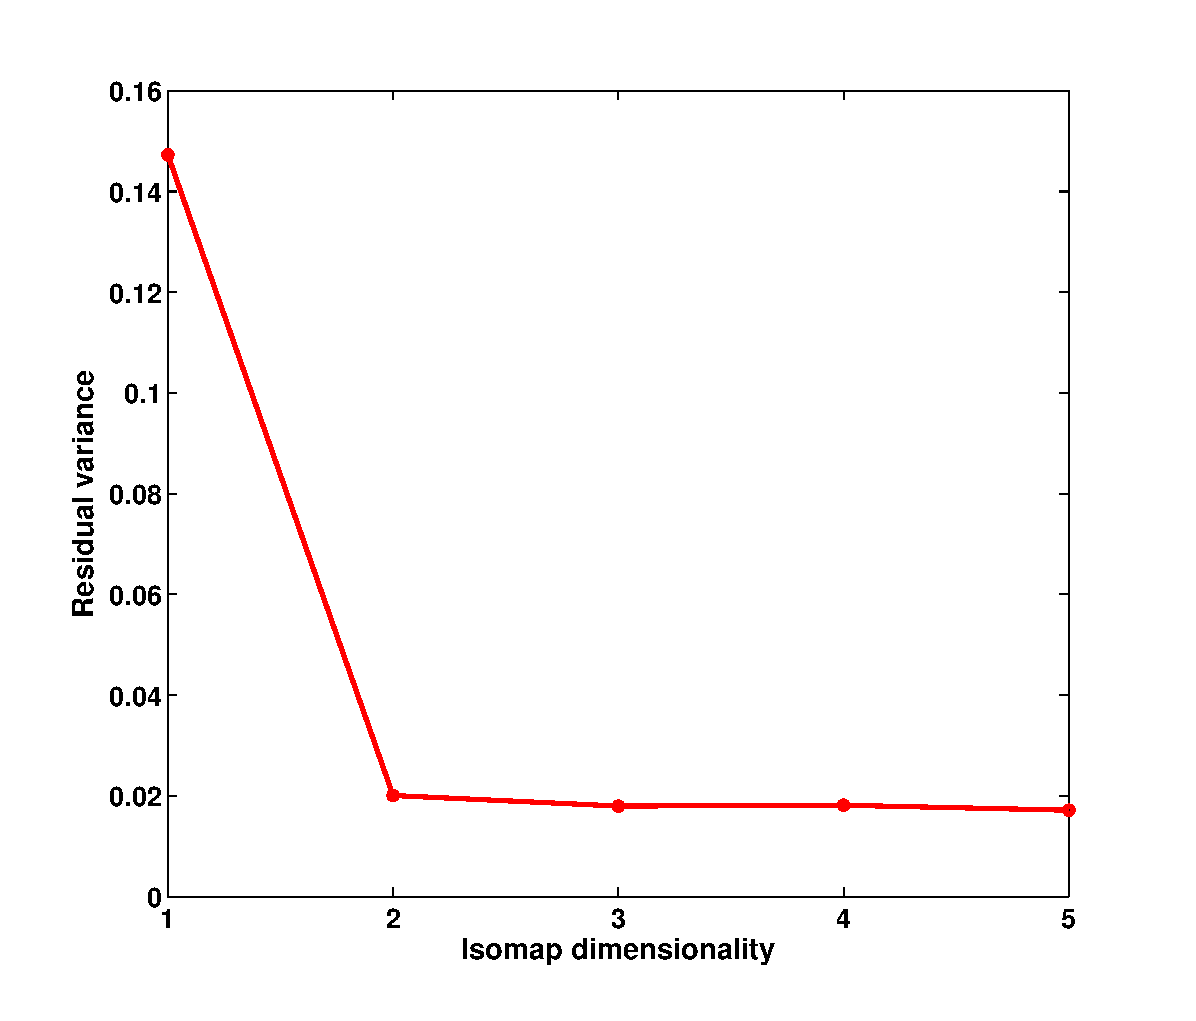
\includegraphics[width=40mm, height=35mm] {dia/gt11cluster4rv.eps}
        \label{gt11clustersRV}
      }
      \subfigure[Explained variance.] {
        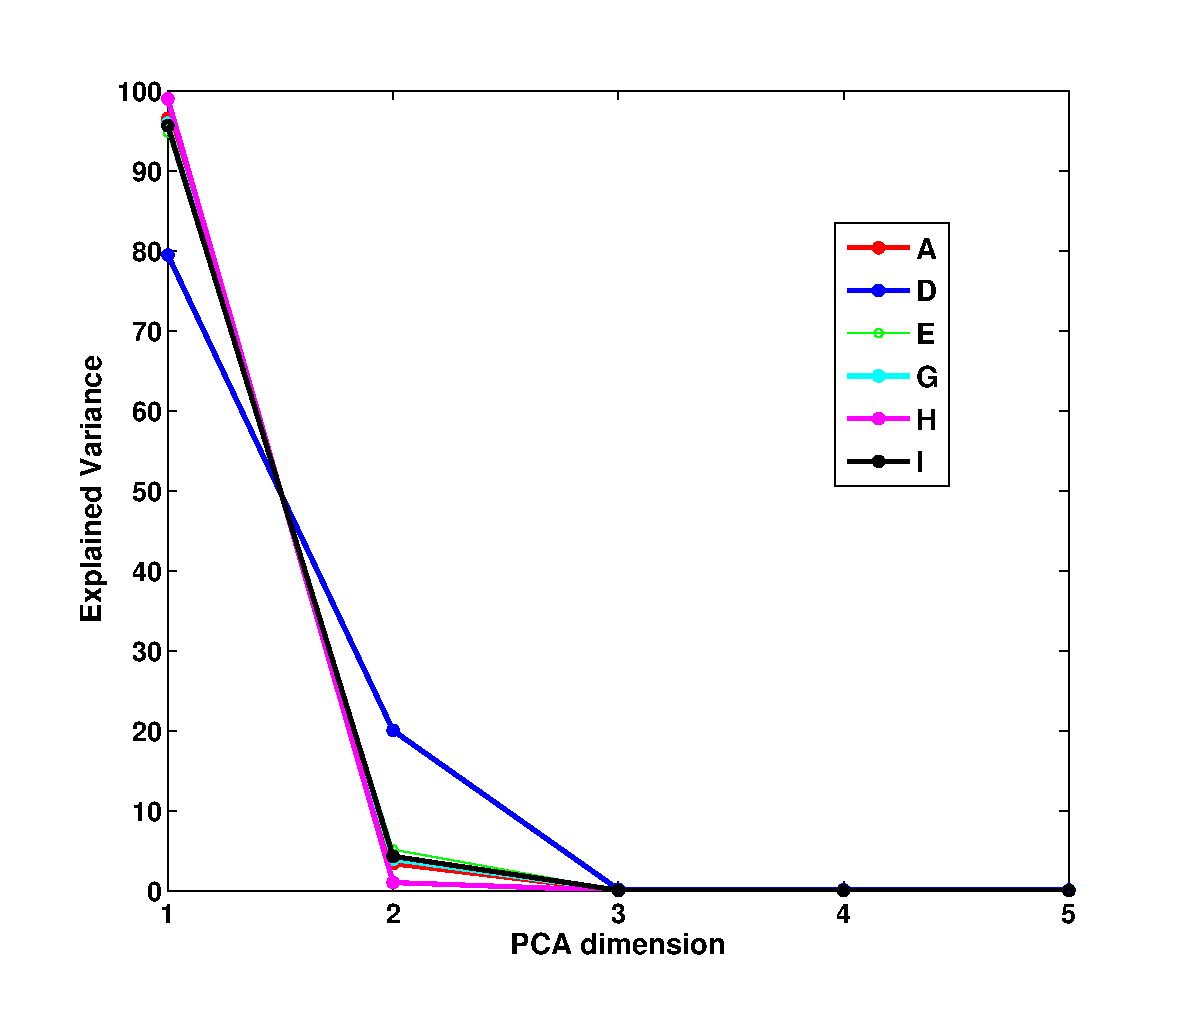
\includegraphics[width=40mm, height=35mm] {dia/gt11clustersEV.eps}
        \label{gt11clustersEV}
      }
      \label{gt11vars}
    \end{center}
  \end{figure}


\end{frame}


\begin{frame}
  \frametitle{Principal components of the clusters}

{\tiny
\begin{table}[!ht]
  \centering
  \begin{tabular}{|c|c|c|c|c|c|c|c|c|c|c|c|}
    \hline
    \multirow{2}{*}{\textbf{A}}   & $p$ & \cellcolor[gray]{0.45} $t_8$ & \cellcolor[gray]{0.50} $t_9$  & $m$ & \cellcolor[gray]{0.65} $t_7$ & \cellcolor[gray]{0.60} $t_4$ & \cellcolor[gray]{0.70} $t_5$ & \cellcolor[gray]{0.75} $t_6$ & \cellcolor[gray]{0.40} $t_1$ & \cellcolor[gray]{0.80} $t_3$ & \cellcolor[gray]{0.55} $t_2$ \\
    & 0.99  & 0.04  & 0.02 & 0.02 & 0.01 & 0.01 & 0.01 & 0.01 & 0.00 & 0.00 & 0.00 \\
    \hline
    \multirow{2}{*}{\textbf{B}}   & $p$ & \cellcolor[gray]{0.45} $t_8$ &  $m$  & \cellcolor[gray]{0.50}$t_9$ & \cellcolor[gray]{0.65} $t_7$ & \cellcolor[gray]{0.60} $t_4$ & \cellcolor[gray]{0.70} $t_5$ & \cellcolor[gray]{0.75} $t_6$ & \cellcolor[gray]{0.40} $t_1$ & \cellcolor[gray]{0.80} $t_3$ & \cellcolor[gray]{0.55} $t_2$ \\
    & 0.99 & 0.01 & 0.01 & 0.01 &  0.00 & 0.00 & 0.00 & 0.00 & 0.00 & 0.00 & 0.00 \\
    \hline
    \multirow{2}{*}{\textbf{C}} & $p$ & \cellcolor[gray]{0.45} $t_8$ & \cellcolor[gray]{0.50} $t_9$ &  $m$ & \cellcolor[gray]{0.65} $t_7$ & \cellcolor[gray]{0.60} $t_4$ & \cellcolor[gray]{0.70} $t_5$ & \cellcolor[gray]{0.75} $t_6$ & \cellcolor[gray]{0.40} $t_1 $ & -- & -- \\
    & 0.99 & 0.02 & 0.01 & 0.01 & 0.01 & 0.01 & 0.01 & 0.01 & 0.01 & 0 & 0 \\
    \hline
    \multirow{4}{*}{\textbf{D}} & $p$ & \cellcolor[gray]{0.45} $t_8$ & \cellcolor[gray]{0.50} $t_9$ &  \cellcolor[gray]{0.65} $t_7$ & $m$ & \cellcolor[gray]{0.60} $t_4$ & \cellcolor[gray]{0.70} $t_5$ & \cellcolor[gray]{0.75} $t_6$ &\cellcolor[gray]{0.40} $t_1$ &\cellcolor[gray]{0.80} $t_3$ & \cellcolor[gray]{0.55} $t_2$ \\
    & 0.99 & 0.07 & 0.06 & 0.03 & 0.03 & 0.03 & 0.03 & 0.02 & 0.02 & 0.00 & 0.00 \\ 
    \cline{2-12}
    & \cellcolor[gray]{0.45} $t_8$ & \cellcolor[gray]{0.50} $t_9$ & \cellcolor[gray]{0.65} $t_7$ &  \cellcolor[gray]{0.60} $t_4$ & \cellcolor[gray]{0.70} $t_5$ & \cellcolor[gray]{0.75} $t_6$ & \cellcolor[gray]{0.40} $t_1$ & $p$ & $m$ & \cellcolor[gray]{0.80} $t_3$ & \cellcolor[gray]{0.55} $t_2$ \\
    & -0.64 & -0.46 & -0.32 & -0.29 & -0.26 & -0.24 & 0.17 & 0.12 & 0.02 & 0.00 & 0.00 \\
    \hline
    \multirow{2}{*}{\textbf{E}} & $p$ & \cellcolor[gray]{0.45} $t_8$ & \cellcolor[gray]{0.50} $t_9$ &  \cellcolor[gray]{0.65} $t_7$ & \cellcolor[gray]{0.70} $t_5$ & \cellcolor[gray]{0.60} $t_4$ & \cellcolor[gray]{0.75} $t_6$ & $m$ & \cellcolor[gray]{0.40} $t_1$ & \cellcolor[gray]{0.80} $t_3$ & \cellcolor[gray]{0.55} $t_2$ \\
    & 0.99 & 0.07 & 0.05 & 0.03 & 0.02 & 0.02 & 0.02 & 0.01 & 0.01 & 0.00 & 0.00 \\ 
    \hline
    \multirow{2}{*}{\textbf{F}} & $p$ & \cellcolor[gray]{0.45} $t_8$ & \cellcolor[gray]{0.50} $t_9$ &  \cellcolor[gray]{0.65} $t_7$ & \cellcolor[gray]{0.60} $t_4$ & \cellcolor[gray]{0.75} $t_6$ & \cellcolor[gray]{0.70} $t_5$ & \cellcolor[gray]{0.40} $t_1$ & $m$ & \cellcolor[gray]{0.55} $t_2$ & \cellcolor[gray]{0.80} $t_3$ \\
    & 0.99 & 0.03 & 0.02 & 0.01 & 0.01 & 0.01 & 0.01 & 0.01 & 0.0 & 0.0 & 0.0 \\ 
    \hline
    \multirow{2}{*}{\textbf{G}} & $p$ & \cellcolor[gray]{0.45} $t_8$ & \cellcolor[gray]{0.50} $t_9$ & \cellcolor[gray]{0.65} $t_7$ & \cellcolor[gray]{0.75} $t_6$ & \cellcolor[gray]{0.60} $t_4$ & \cellcolor[gray]{0.70} $t_5$ & \cellcolor[gray]{0.40} $t_1$ & $m$ & \cellcolor[gray]{0.80} $t_3$ & \cellcolor[gray]{0.55} $t_2$ \\
    & 0.99 & 0.07 & 0.05 & 0.04 & 0.03 & 0.03 & 0.03 & 0.02 & 0.01 & 0.0 & 0.0 \\ 
    \hline
    \multirow{2}{*}{\textbf{H}} & $p$ & \cellcolor[gray]{0.45} $t_8$ & \cellcolor[gray]{0.50} $t_9$ & \cellcolor[gray]{0.60} $t_4$ &\cellcolor[gray]{0.65} $t_7$ &\cellcolor[gray]{0.70} $t_5$ &\cellcolor[gray]{0.75} $t_6$ &\cellcolor[gray]{0.40} $t_1$ & $m$ & -- & -- \\
    & 0.99 & 0.04 & 0.03 & 0.02 & 0.01 & 0.01 & 0.01 & 0.01 & 0.00 & 0 & 0 \\ 
    \hline
    \multirow{2}{*}{\textbf{I}} & $p$ &\cellcolor[gray]{0.45} $t_8$ & \cellcolor[gray]{0.50} $t_9$ & \cellcolor[gray]{0.65} $t_7$ &\cellcolor[gray]{0.60} $t_4$ &\cellcolor[gray]{0.70} $t_5$ &\cellcolor[gray]{0.75} $t_6$ &\cellcolor[gray]{0.40} $t_1$ & $m$ & -- & -- \\
    & 0.98 & 0.10 & 0.07 & 0.05 & 0.04 & 0.04 & 0.04 & 0.03 & 0.01 & 0 & 0 \\ 
    \hline
    \multirow{2}{*}{\textbf{J}} & $p$ &\cellcolor[gray]{0.45} $t_8$ &\cellcolor[gray]{0.50} $t_9$ & \cellcolor[gray]{0.65} $t_7$ & \cellcolor[gray]{0.60} $t_4$ &\cellcolor[gray]{0.75} $t_6$ &\cellcolor[gray]{0.70} $t_5$ &\cellcolor[gray]{0.40} $t_1$ &\cellcolor[gray]{0.80} $t_3$ &\cellcolor[gray]{0.55} $t_2$ & $m$ \\
    & 0.97 & 0.13 & 0.10 & 0.06 & 0.06 & 0.05 & 0.05 & 0.03 & 0.0 & 0.0 & 0 \\ 
    \hline
    \multirow{2}{*}{\textbf{K}} & $p$ &\cellcolor[gray]{0.45} $t_8$ & \cellcolor[gray]{0.50} $t_9$ & \cellcolor[gray]{0.65} $t_7$ &\cellcolor[gray]{0.60} $t_4$ &\cellcolor[gray]{0.70} $t_5$ &\cellcolor[gray]{0.75} $t_6$ &\cellcolor[gray]{0.40} $t_1$ &\cellcolor[gray]{0.80} $t_3$ &\cellcolor[gray]{0.55} $t_2$ & $m$ \\
    & 0.85 & 0.33 & 0.25 & 0.17 & 0.14 & 0.13 & 0.13 & 0.09 & -0.00 & -0.00 & 0 \\ 
    \hline
  \end{tabular}
  \label{gt11pcTopWeights}
\end{table}
}


{\tiny
\begin{table}[!ht]
  \centering
  \begin{tabular}{|c|c|c|c|c|c|c|c|c|c|}
    \hline
    Gear pair No. & \cellcolor[gray]{0.40} 1 & \cellcolor[gray]{0.45} 8 & \cellcolor[gray]{0.50} 9 & \cellcolor[gray]{0.55} 2 & \cellcolor[gray]{0.60} 4 & \cellcolor[gray]{0.65} 7 & \cellcolor[gray]{0.70} 5 &\cellcolor[gray]{0.75} 6 & \cellcolor[gray]{0.80} 3\\
    \hline
    I/O Speed ratio & \cellcolor[gray]{0.40} 0.35 & \cellcolor[gray]{0.45} 0.46 & \cellcolor[gray]{0.50} 0.54 & \cellcolor[gray]{0.55} 0.76 & \cellcolor[gray]{0.60} 0.86 & \cellcolor[gray]{0.65} 0.97 & \cellcolor[gray]{0.70}0.97 & \cellcolor[gray]{0.75} 1.09 & \cellcolor[gray]{0.80} 1.71\\
    \hline
  \end{tabular}
  \label{iosRatio}
\end{table}
}


\end{frame}


\begin{frame}
  \frametitle{Discussion}
  
  \begin{itemize}
  \item Gear-pairs in the final transmission stage are under the highest
    stress, hence vary the most with increasing power.
  \item Gear-pairs with lower input to output speed ratios are at higher
    stress, hence vary more in the same transmission stage.
  \item Gearbox with higher power requirements use larger modules.
  \end{itemize}


  \begin{figure}[ht]\begin{center}
      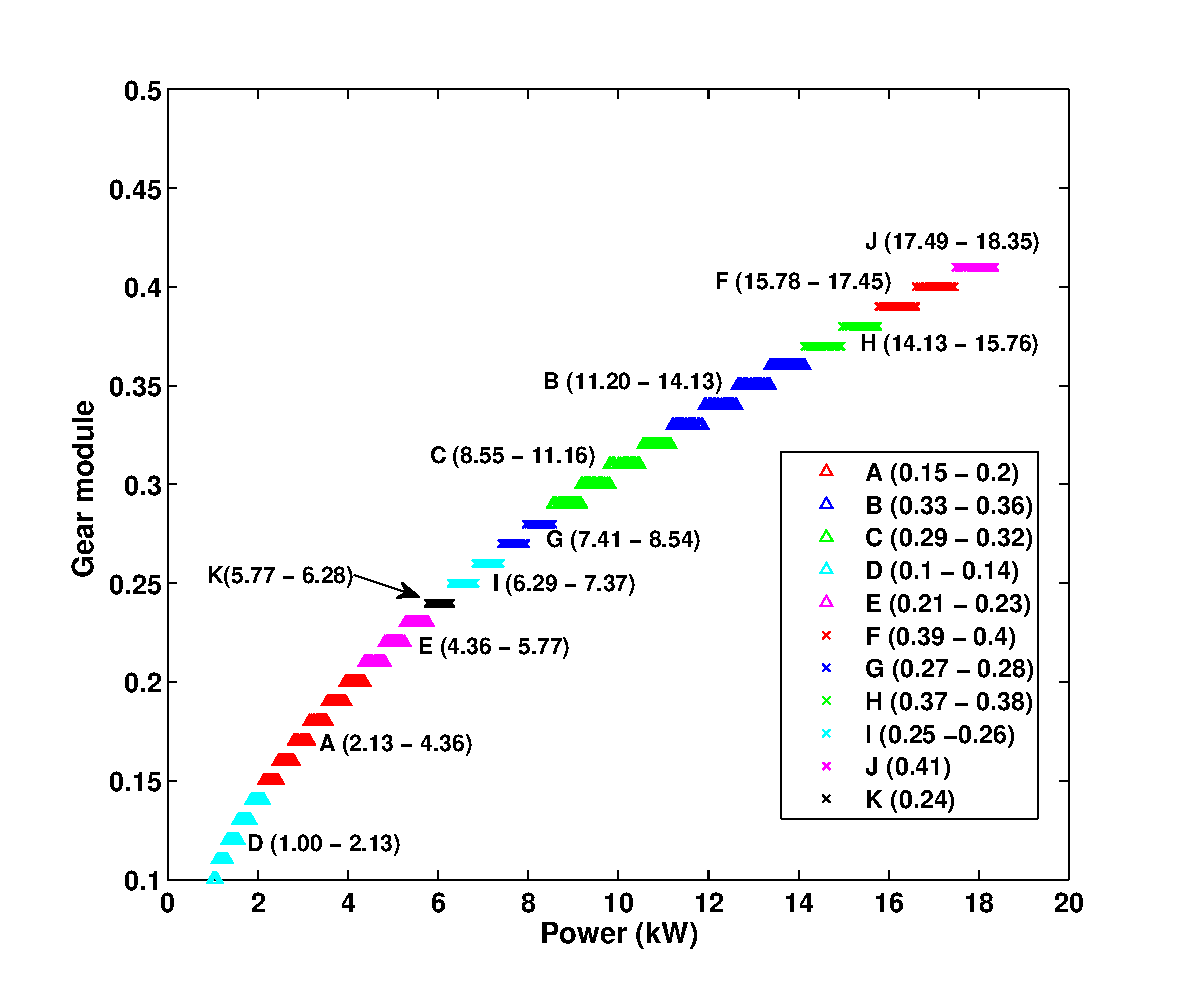
\includegraphics[width=40mm, height=35mm]{dia/gt11pVsm.eps}
      \label{gt11pVsm}
    \end{center}
  \end{figure}

\end{frame}


\begin{frame}
  \frametitle{Pareto-front and clusters for the full problem}

  \begin{itemize}
  \item 989 optimal solutions 
  \item pareto-frontier is a two dimensional manifold in the objective
    space
  \item 7 clusters.
  \end{itemize}

  \begin{figure}[ht]\begin{center}
      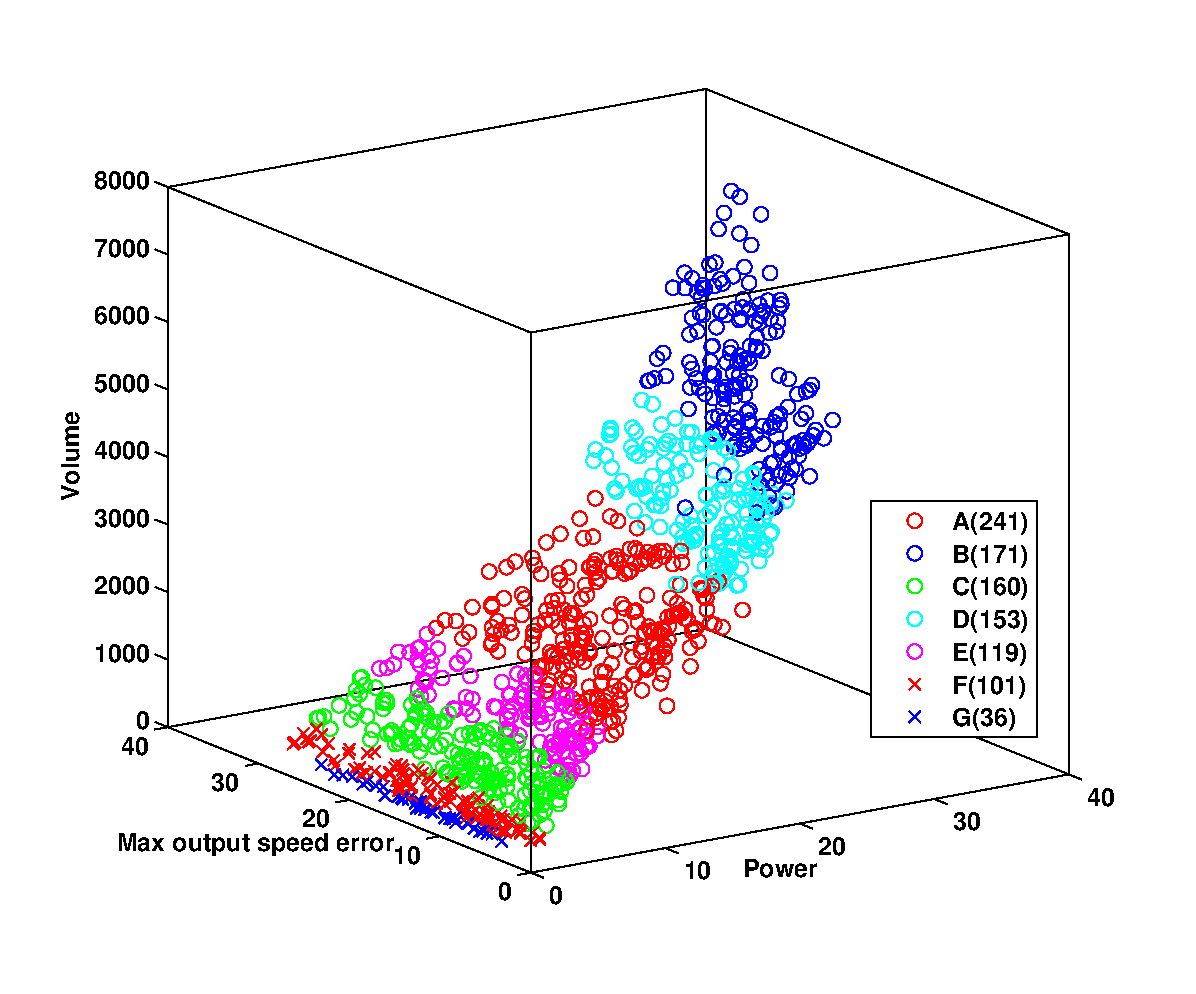
\includegraphics[width=53mm, height=45mm]{dia/gtvopareto2.eps}
      \label{gtvClusters}
    \end{center}
  \end{figure}


\end{frame}



\begin{frame}
  \frametitle{Isomap and PCA analysis}
  
  \begin{itemize}
  \item No clear indication of manifold dimension.
  \item Four principal components with significant explained variance.
  \end{itemize}


  \begin{figure}[ht]
    \begin{center}
      \subfigure[Residual variance] {
        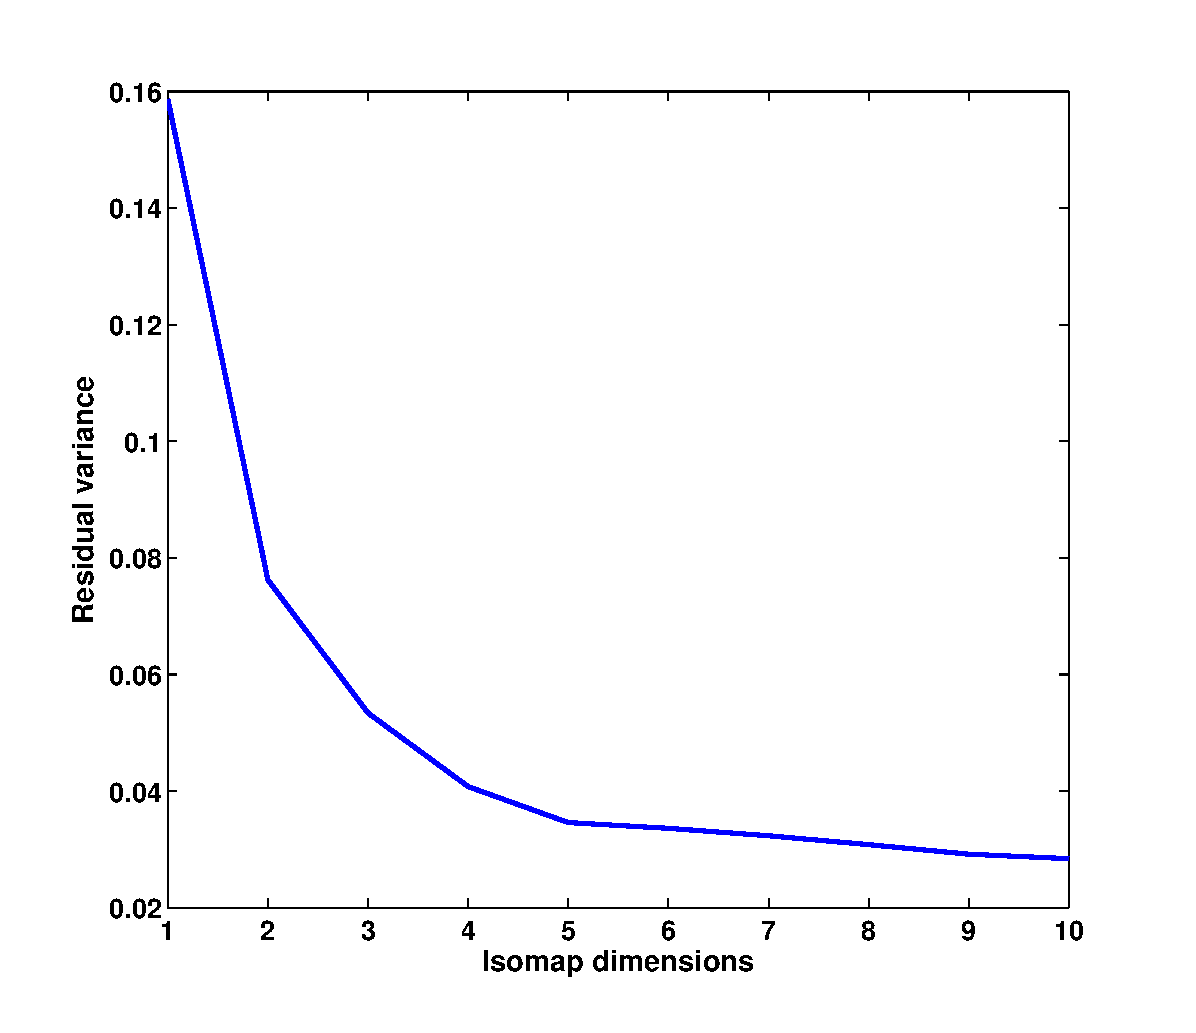
\includegraphics[width=40mm, height=35mm] {dia/gtvorv1.eps}
        \label{gtvrv}
      }
      \subfigure[Explained variance.] {
        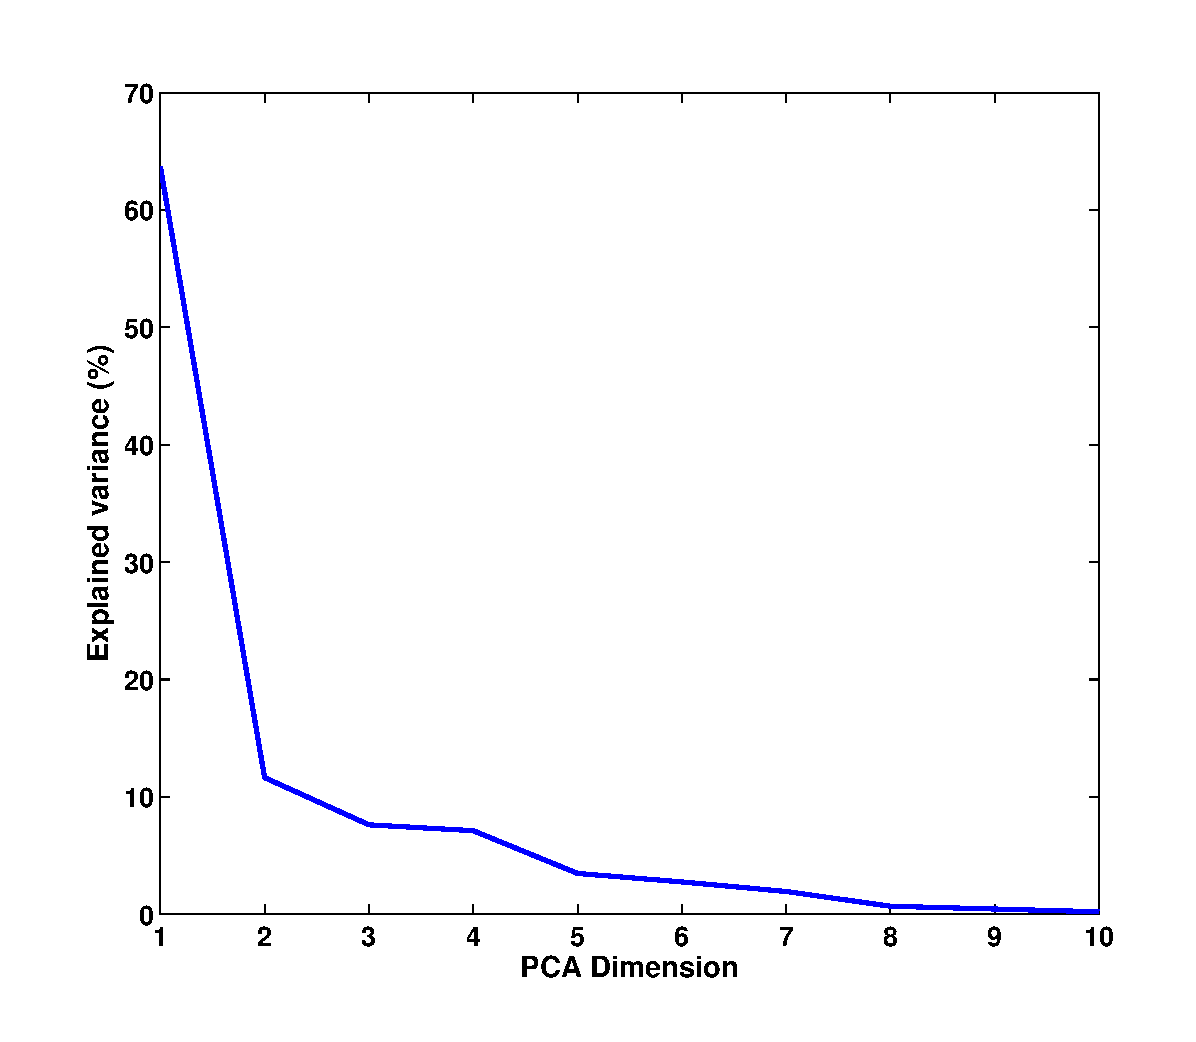
\includegraphics[width=40mm, height=35mm] {dia/gtvWholeEV.eps}
        \label{gtvev}
      }
      \label{gtvovars}
    \end{center}
  \end{figure}


\end{frame}



\begin{frame}
  \frametitle{Isomap residual variances for the clusters}
  
  \begin{itemize}
  \item for most clusters, the largest drop in residual variance is for 
    two or three dimensional embedding.
  \end{itemize}

  \begin{figure}[ht]
    \begin{center}
      \subfigure[Residual variance for A, C, and E.] {
        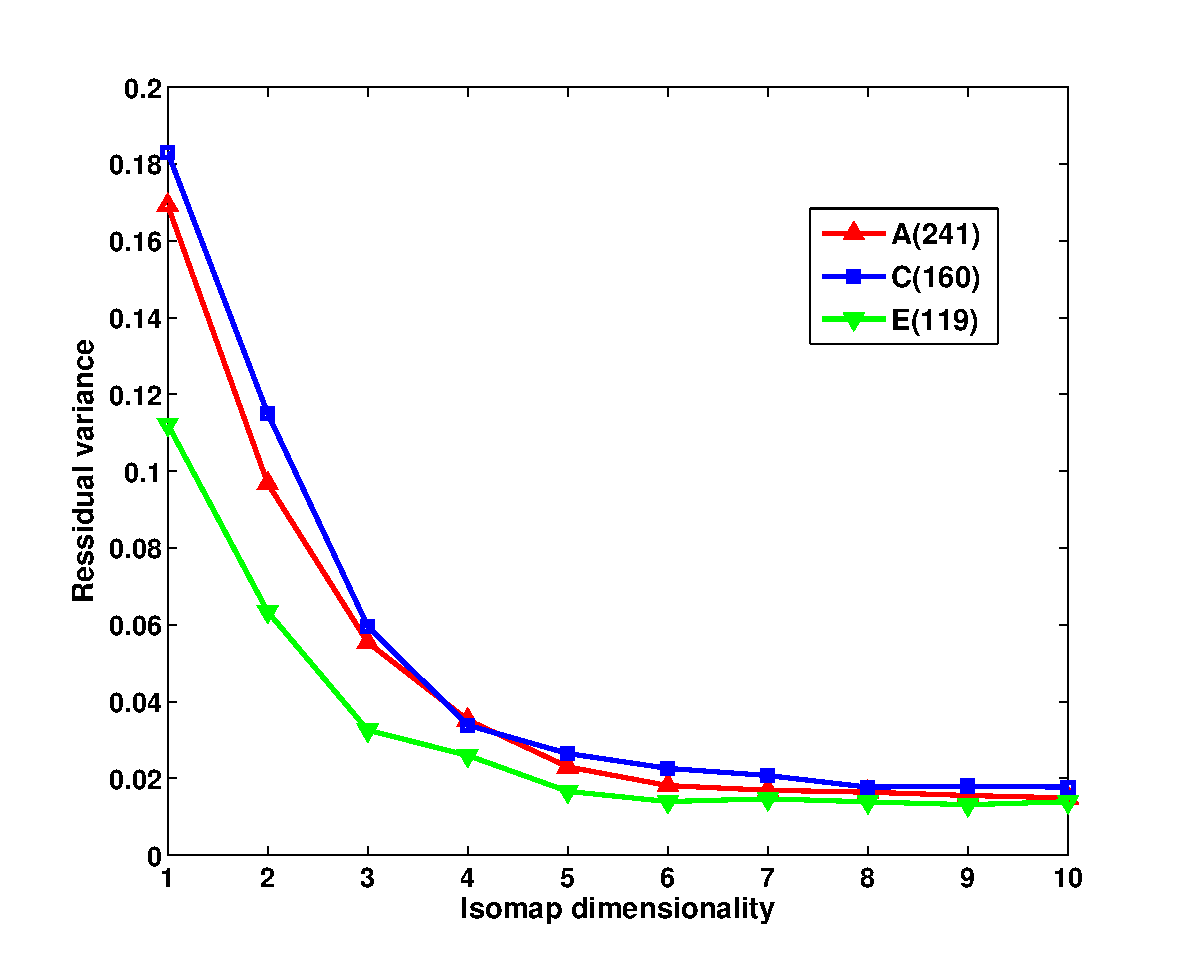
\includegraphics[width=40mm, height=35mm] {dia/gtvcrv1.eps}
        \label{gtvrv}
      }
      \subfigure[Residual variances for B, D, F and G.] {
        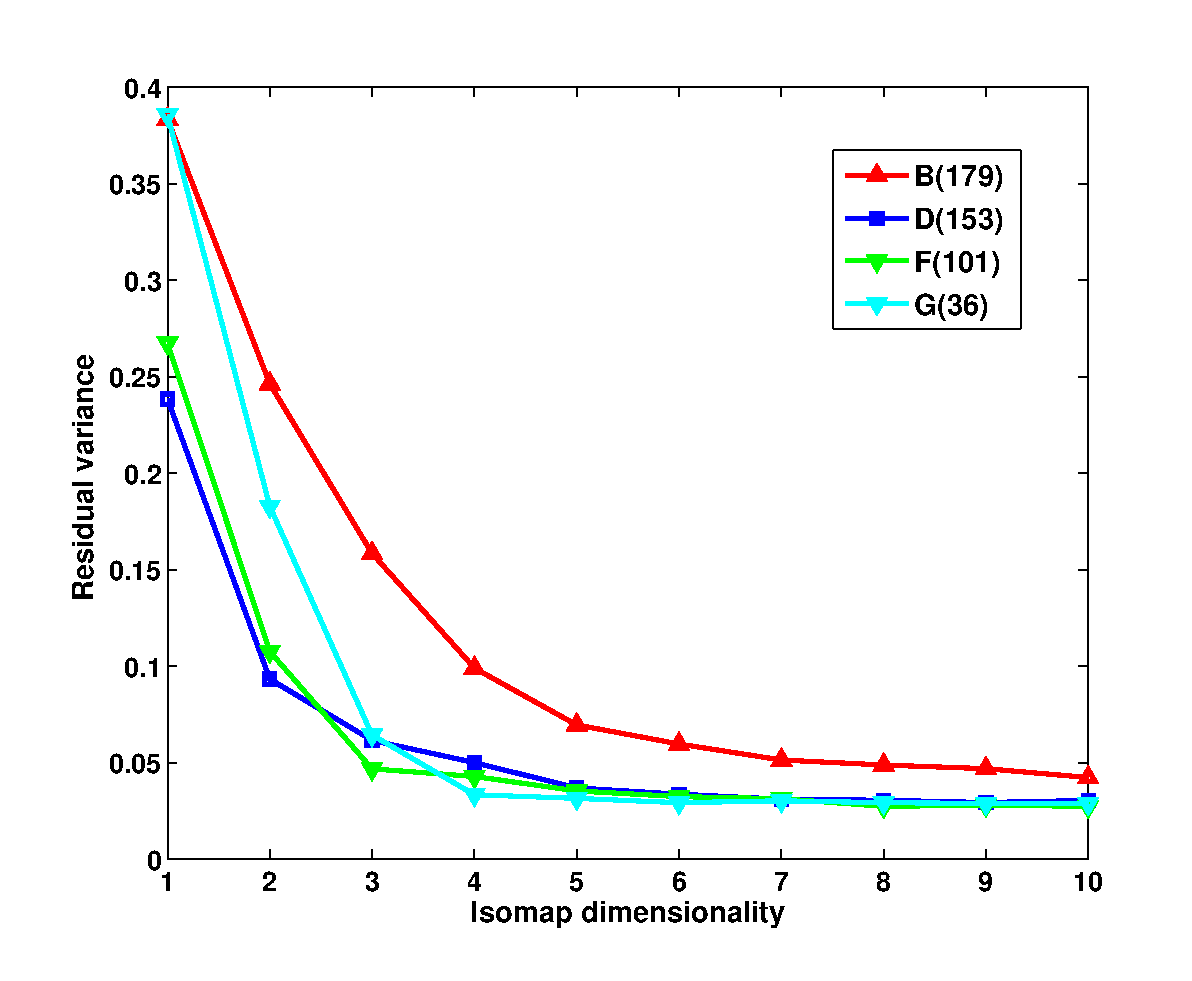
\includegraphics[width=40mm, height=35mm] {dia/gtvcrv2.eps}
        \label{gtvev}
      }
      \label{gtvrvs}
    \end{center}
  \end{figure}



\end{frame}


% \begin{figure}[ht]\begin{center}
%  \subfloat[Clusters \textbf{A}, \textbf{B}, \textbf{C} and \textbf{D}]{
%  \label{gt11rv} 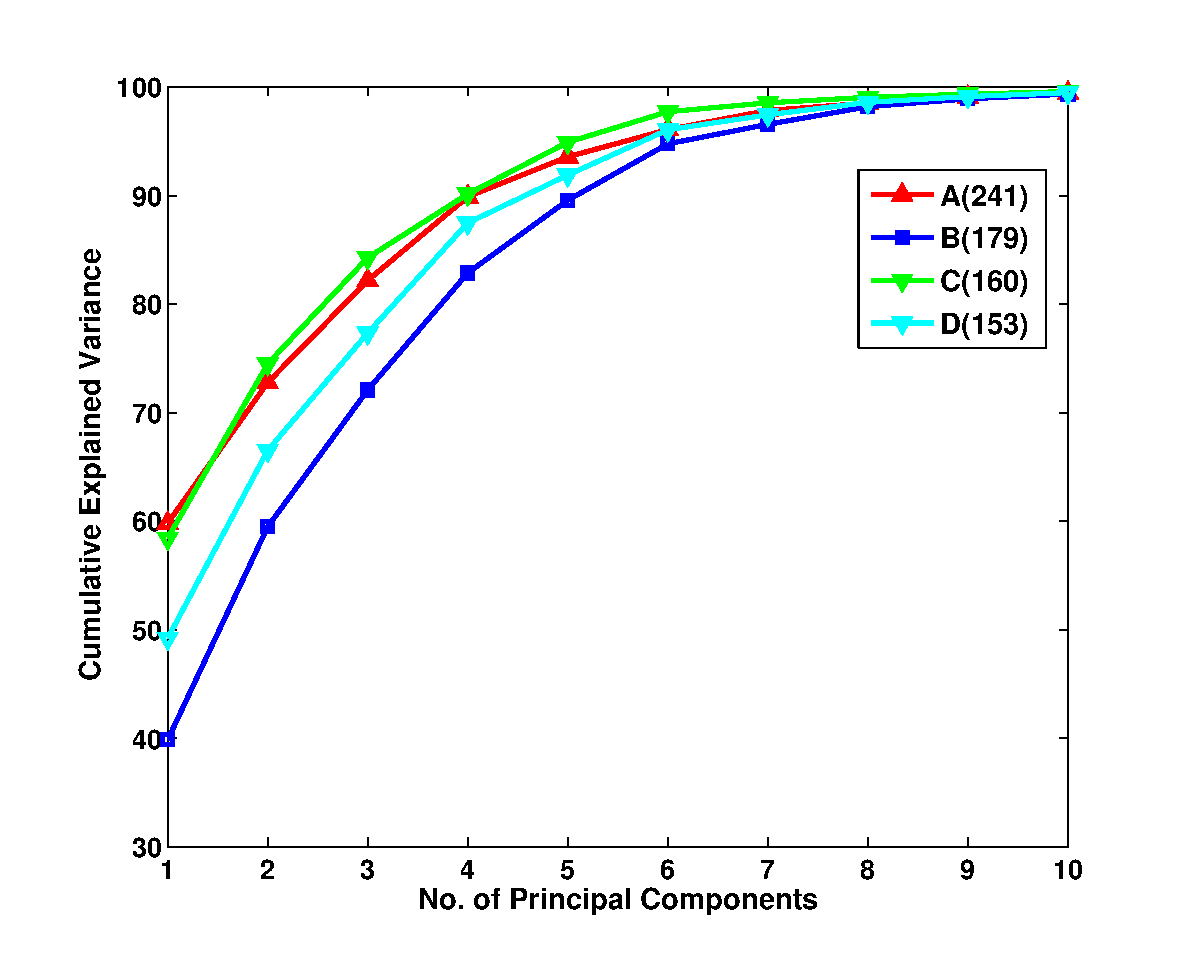
\includegraphics[width=62mm, height=52mm]{dia/gtvicev1.eps}}
%  \subfloat[Clusters \textbf{E}, \textbf{F} and \textbf{G}]{
%  \label{gt11ev} 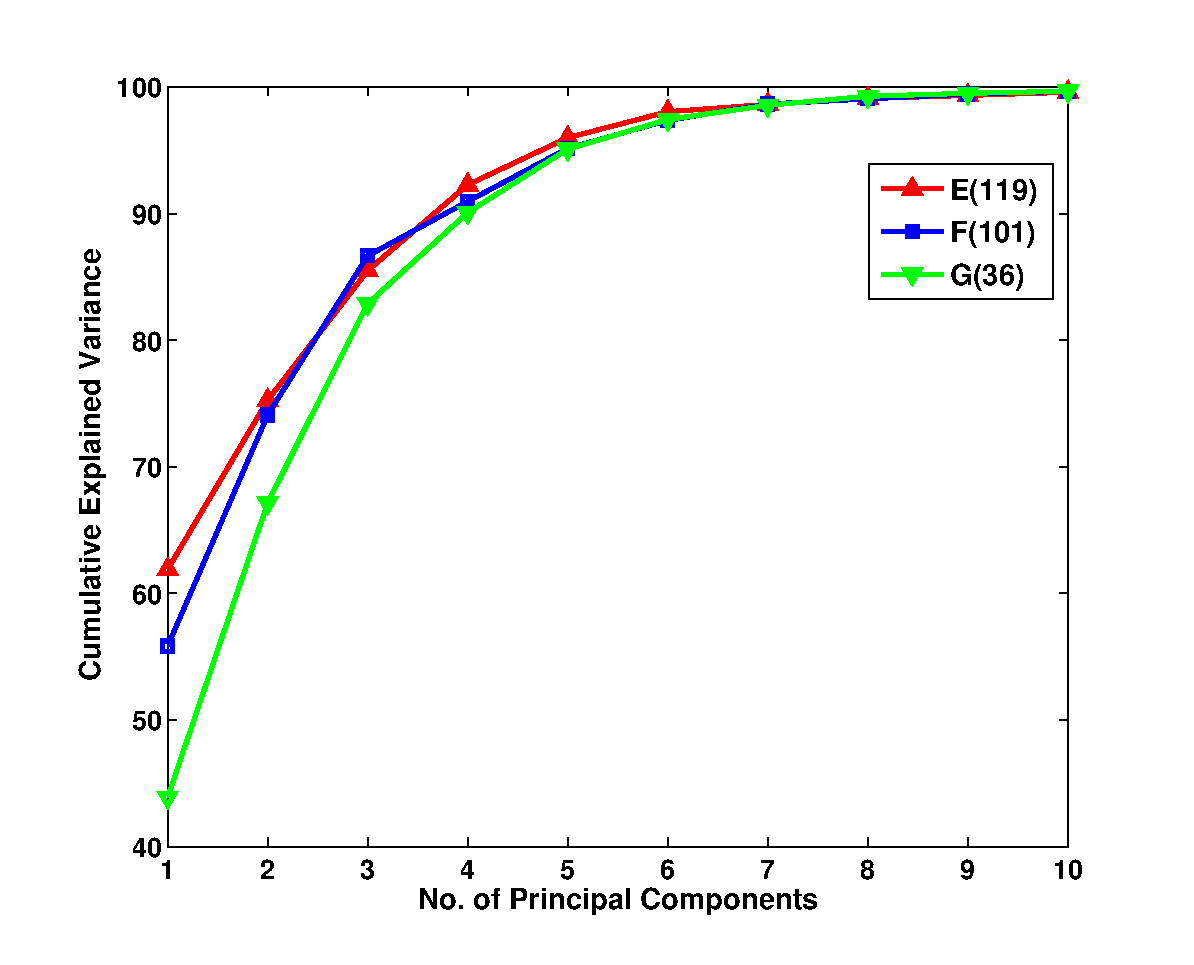
\includegraphics[width=62mm, height=52mm]{dia/gtvicev2.eps}}
%  \caption{Cumulative PCA explained variance for 29 variable problem. For
%   most clusters, first five-six principal components cover 90\% of the
%   explained variance.}
%  \label{gtvClustersEV}
% \end{center}\end{figure}




\begin{frame}
  \frametitle{PCA explained variance for the clusters}
  
  \begin{itemize}
  \item Six or seven principal components account for 90\% variance.
  \end{itemize}

  \begin{figure}[ht]
    \begin{center}
      \subfigure[Cumulative explained variances for A, B, C and D.] {
        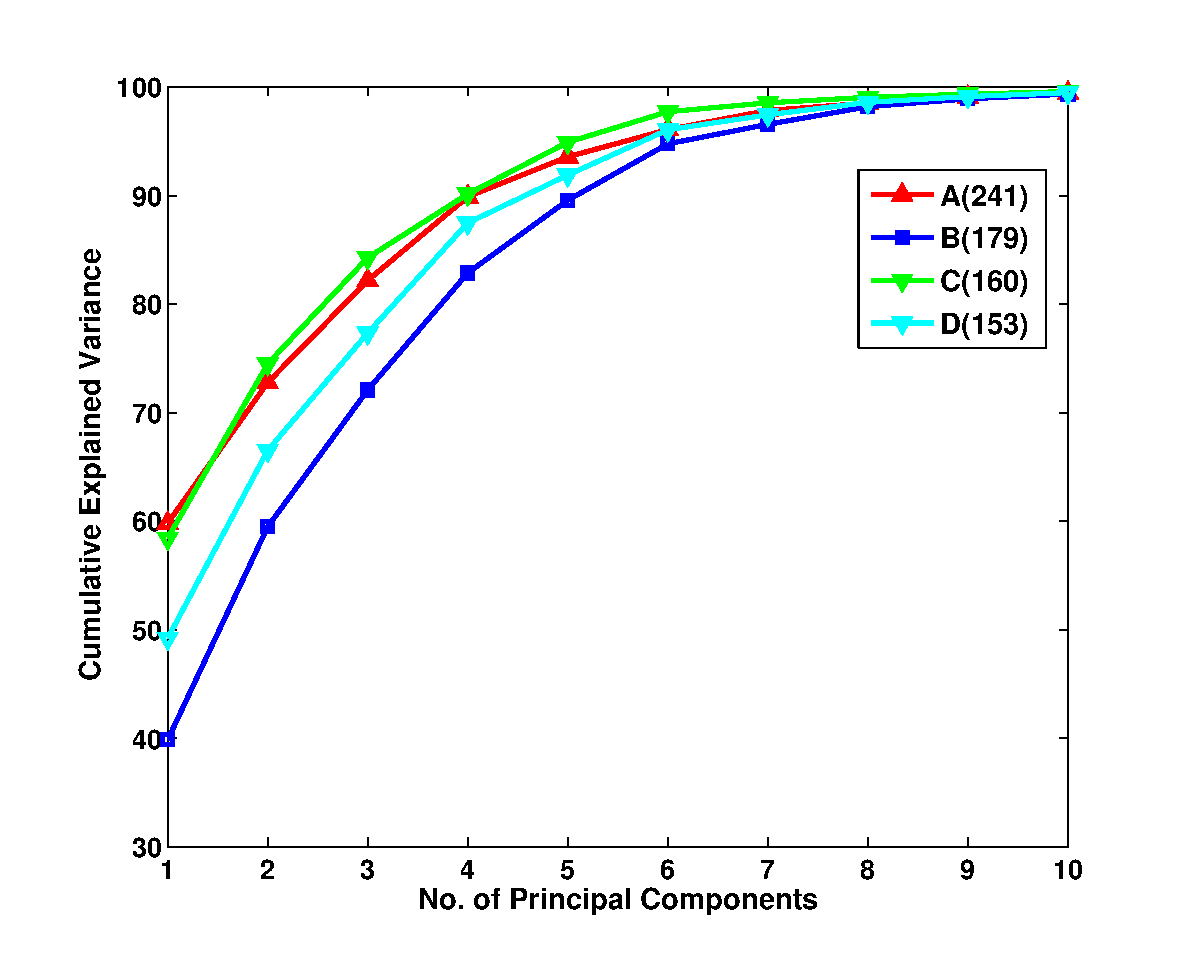
\includegraphics[width=40mm, height=35mm] {dia/gtvicev1.eps}
        \label{gtvrv}
      }
      \subfigure[Cumulative explained variances for E, F and G.] {
        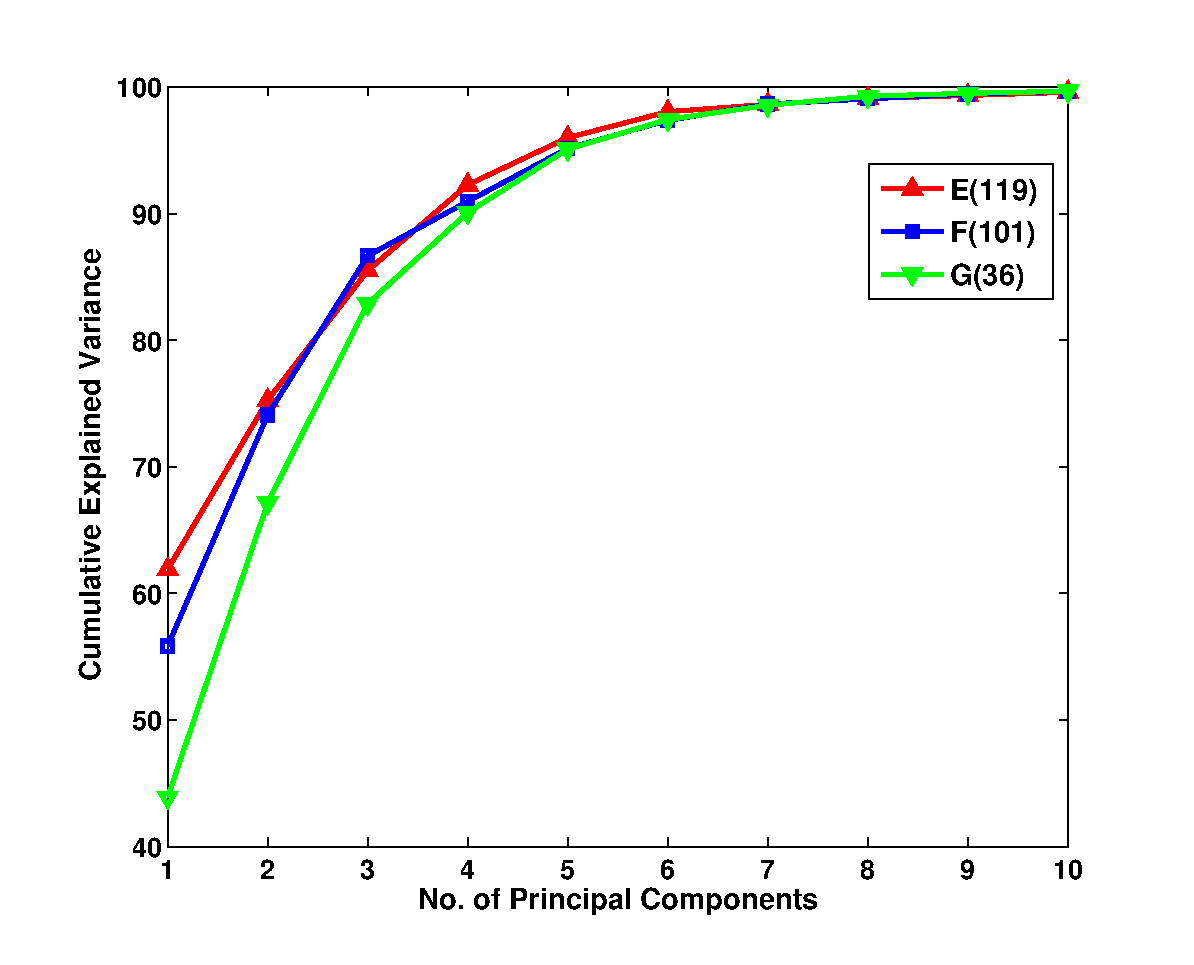
\includegraphics[width=40mm, height=35mm] {dia/gtvicev2.eps}
        \label{gtvev}
      }
      \label{gtvocevs}
    \end{center}
  \end{figure}


\end{frame}




\subsection{C. Clutch brake design problem}


\begin{frame}[allowframebreaks]
  \frametitle{Clutch brake design problem}

  \begin{itemize}
  \item Two objectives:
    \begin{enumerate}[(i)]
    \item minimization of mass, and,
    \item minimization of stopping time.
    \end{enumerate}
  \end{itemize}


  \begin{figure}[ht]\begin{center}
      \fbox{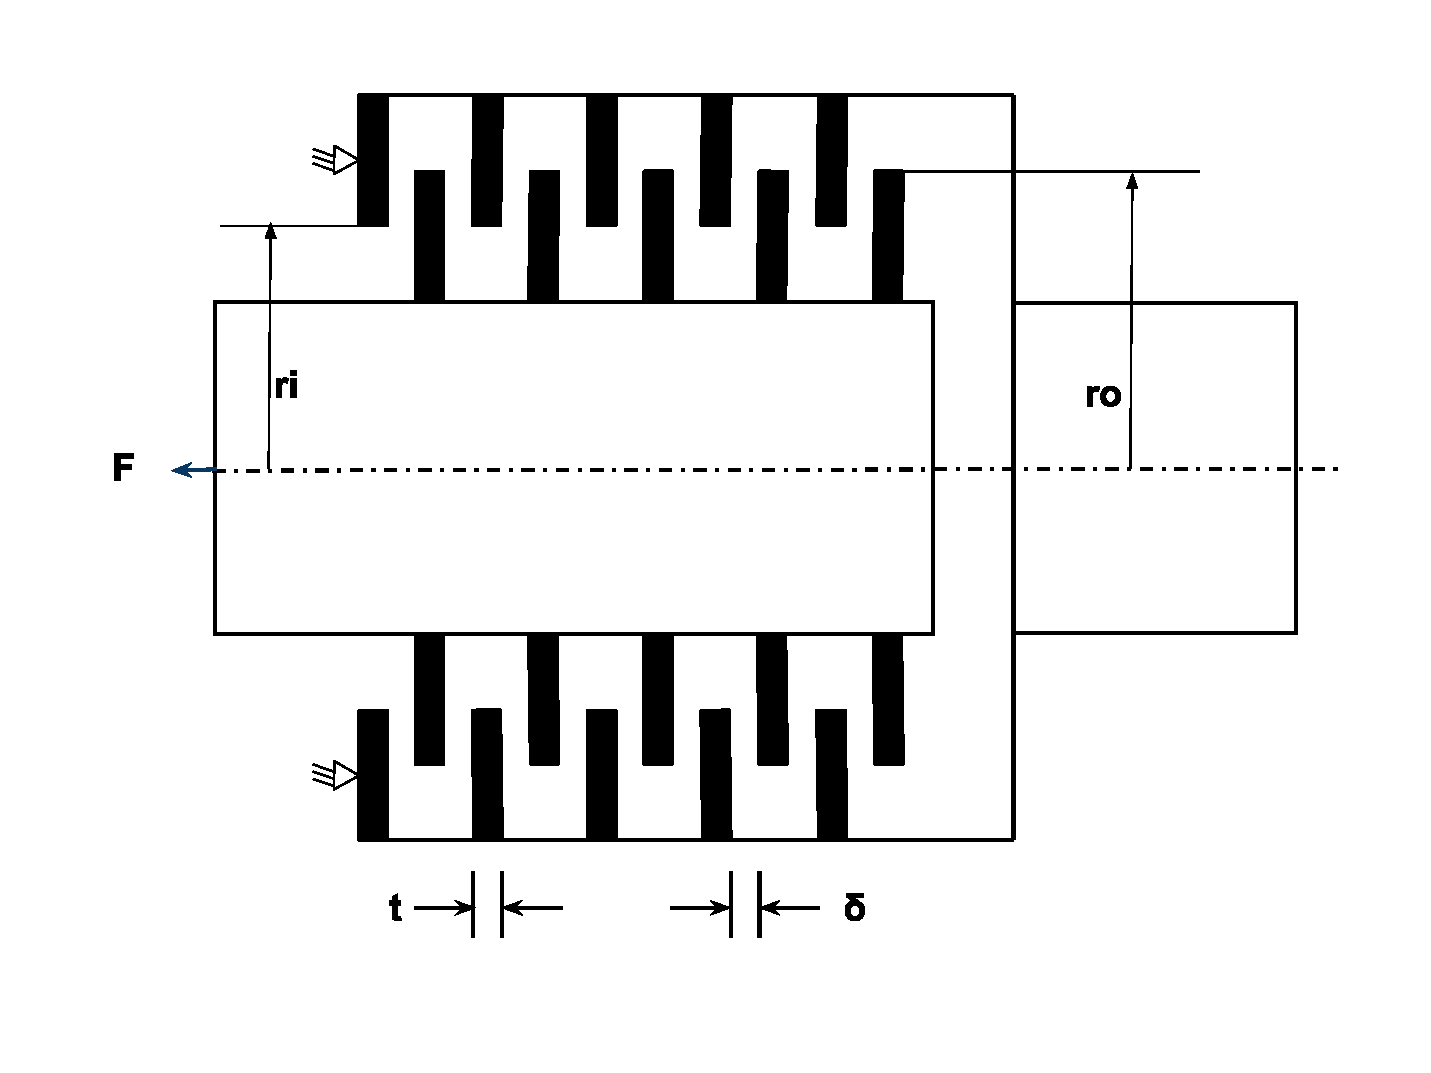
\includegraphics[width=40mm, height=30mm]{dia/clutchbrake.eps}}
      \label{clutchbrake}
    \end{center}
  \end{figure}
  
    

\end{frame}





\begin{frame}
  \frametitle{Pareto-front and clusters}

  \begin{itemize}
  \item 95 pareto-optimal solutions
  \item Six clusters.
  \end{itemize}

  \begin{figure}[ht]
    \begin{center}
      \subfigure[Pareto-front and clusters in the objectives space.] {
        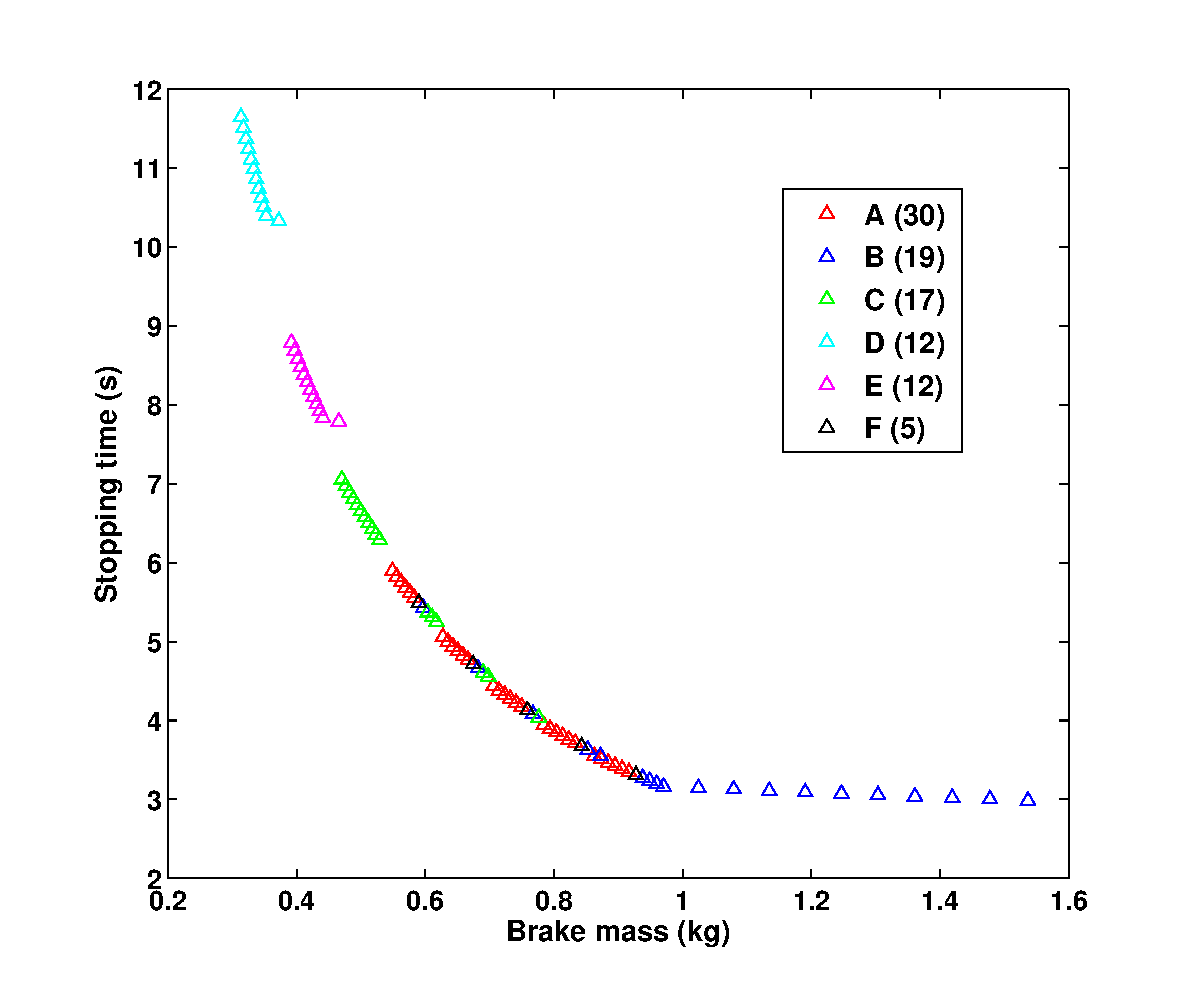
\includegraphics[width=40mm, height=35mm] {dia/clutchParetoClusters.eps}
        \label{clutch}
      }
      \subfigure[Radius vs. no. of friction surfaces.] {
        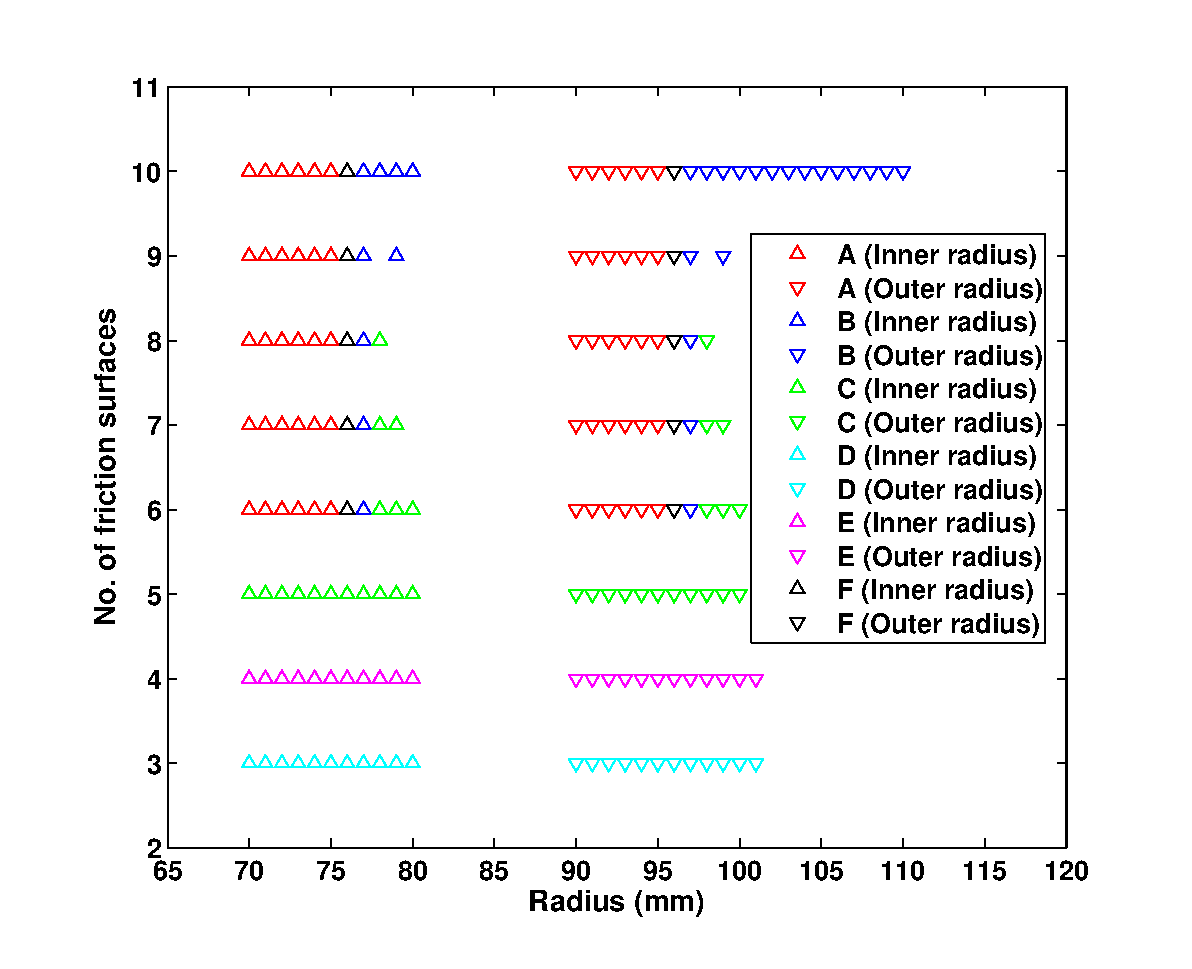
\includegraphics[width=40mm, height=35mm] {dia/clutchrVsZ.eps}
        \label{clutchrVsZ}
      }
      \label{clutchpareto}
    \end{center}
  \end{figure}



\end{frame}

% \begin{figure}[ht]\begin{center}
%  \subfloat[Isomap Residual Variance.]{
%  \label{clutchwrv} 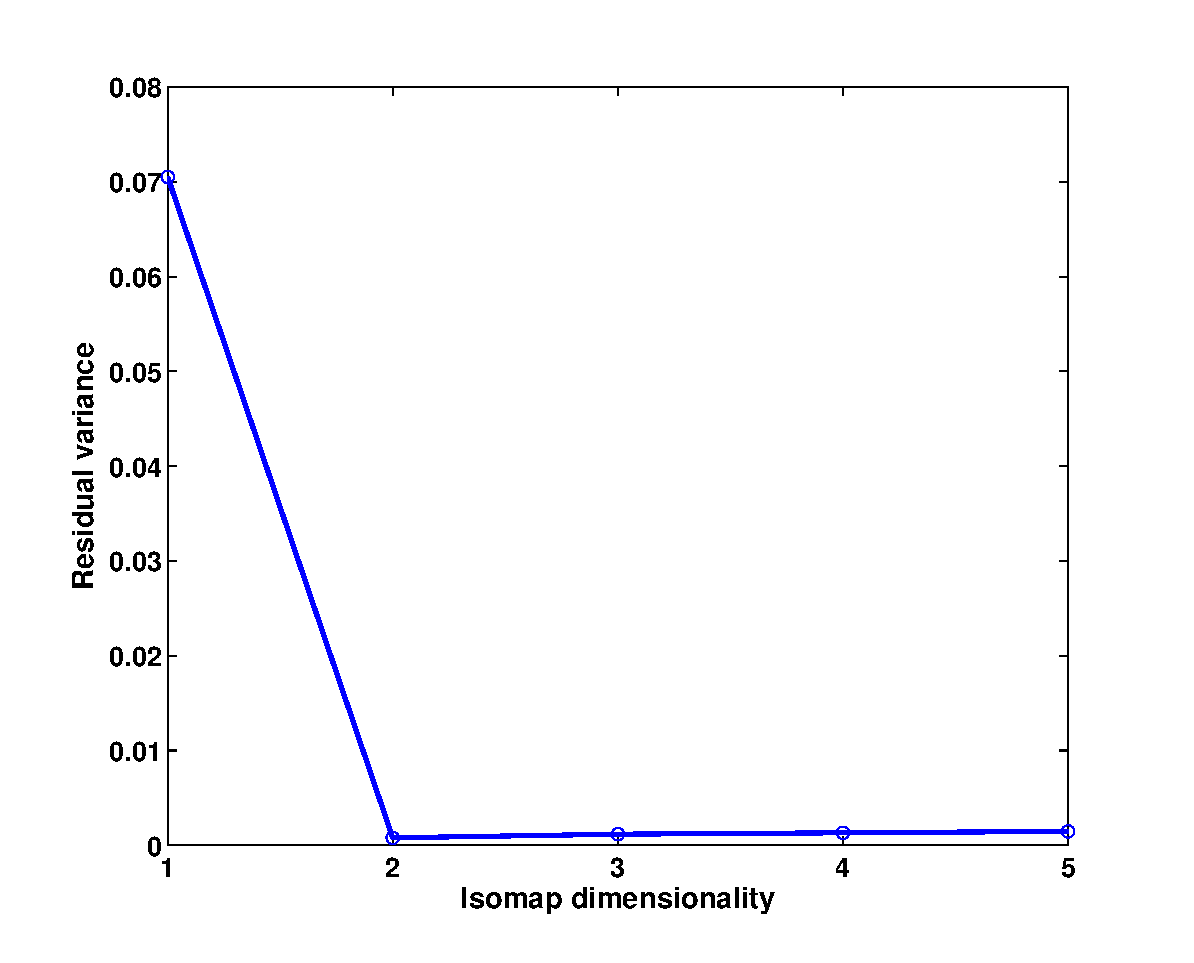
\includegraphics[width=62mm, height=52mm]{dia/clutchRV.eps}}
%  \subfloat[PCA Explained variance.]{
%  \label{clutchwev} 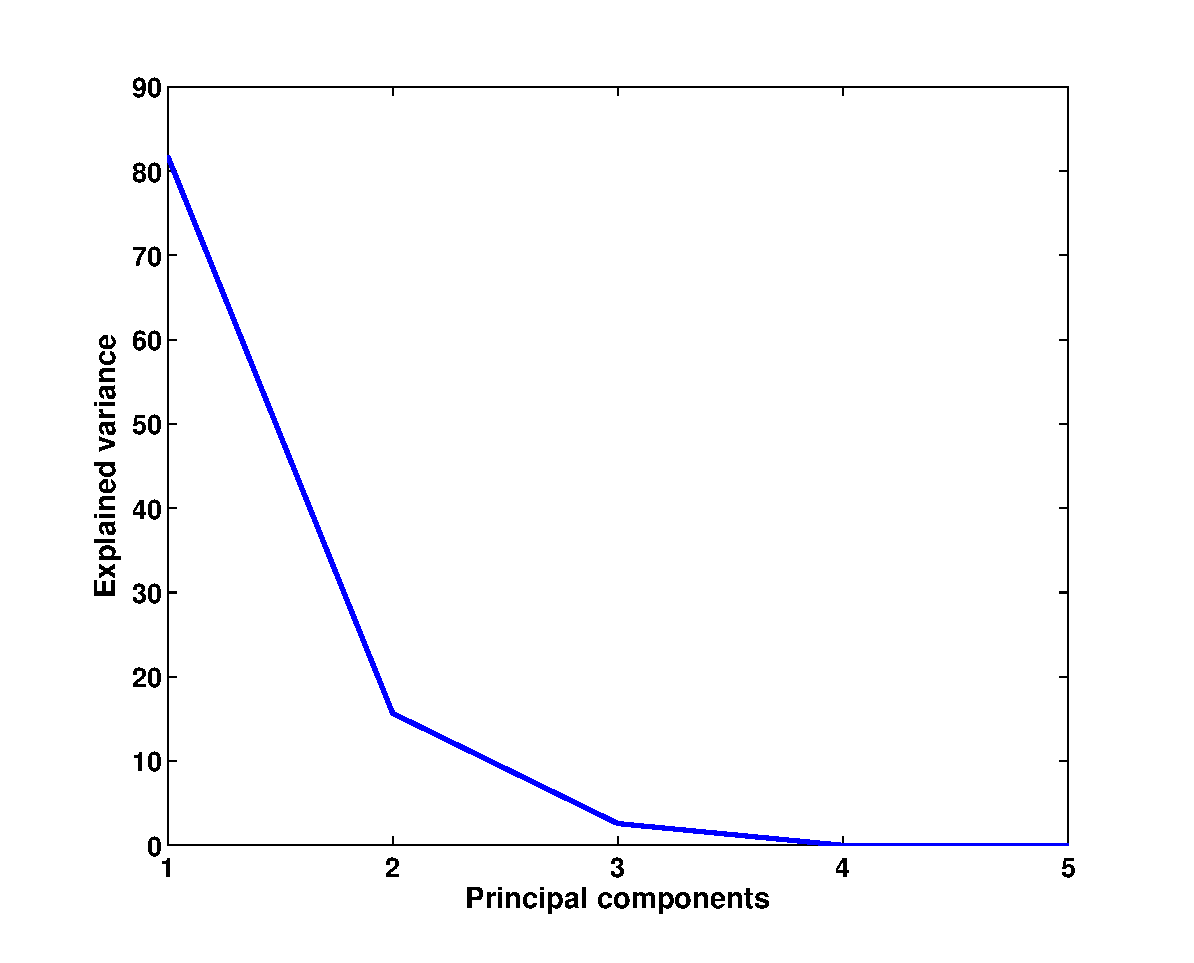
\includegraphics[width=62mm, height=52mm]{dia/clutchEV.eps}}
% \caption{Isomap and PCA results for the pareto-front of multiple-disk
%   clutch brake problem pareto-front. The manifold dimensionality is one as
%   indicated in the Isomap residual variance plot but the PCA explained
%   variance shows two significant principal components.}
%  \label{clutchWholeVar}
% \end{center}\end{figure}


\begin{frame}
  \frametitle{Isomap and PCA analysis of the pareto-front}

  \begin{itemize}
  \item Pareto-front is a one dimensional manifold.
  \item Two significant principal components.
  \end{itemize}

  \begin{figure}[ht]
    \begin{center}
      \subfigure[Residual variance.] {
        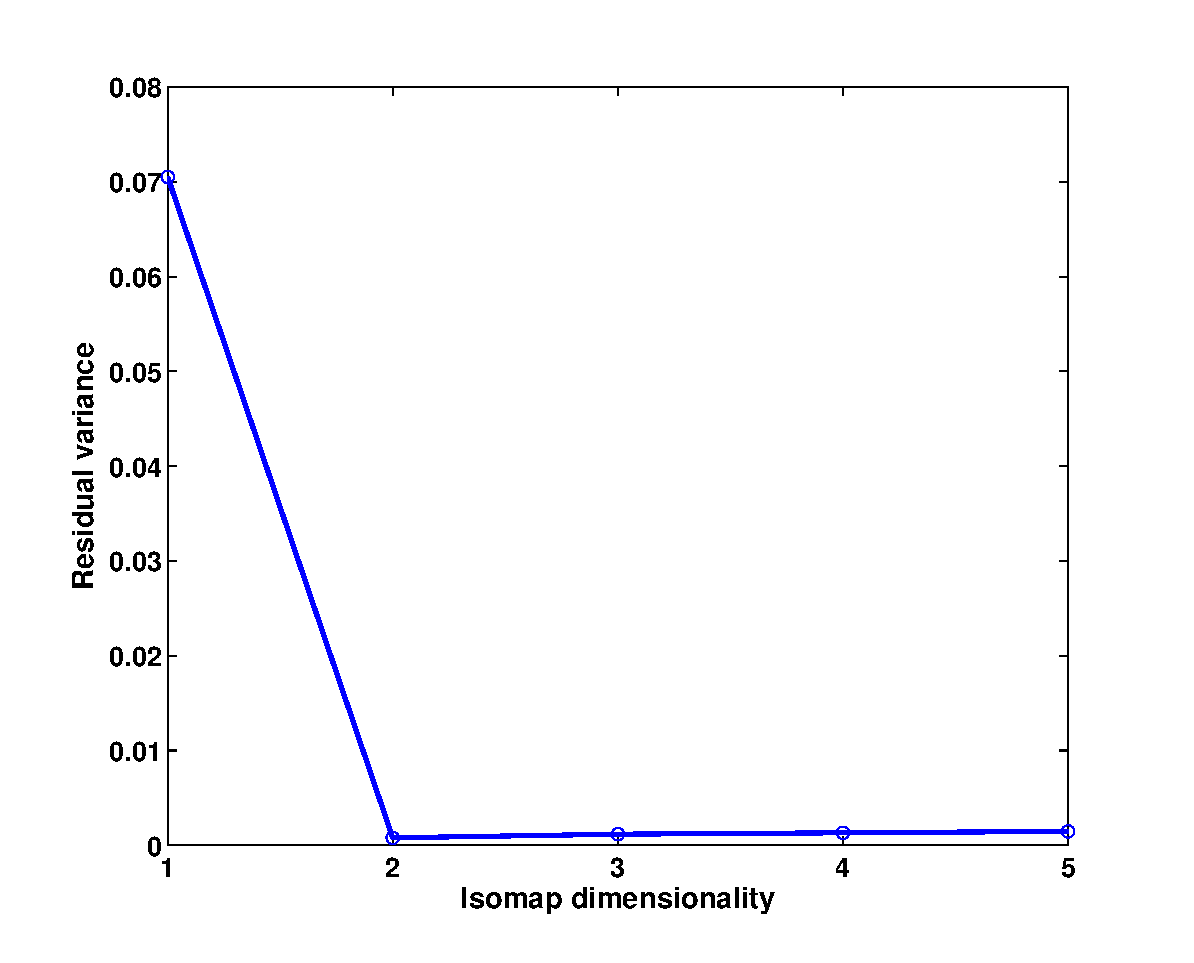
\includegraphics[width=40mm, height=35mm] {dia/clutchRV.eps}
        \label{clutchrv}
      }
      \subfigure[PCA explained variance.] {
        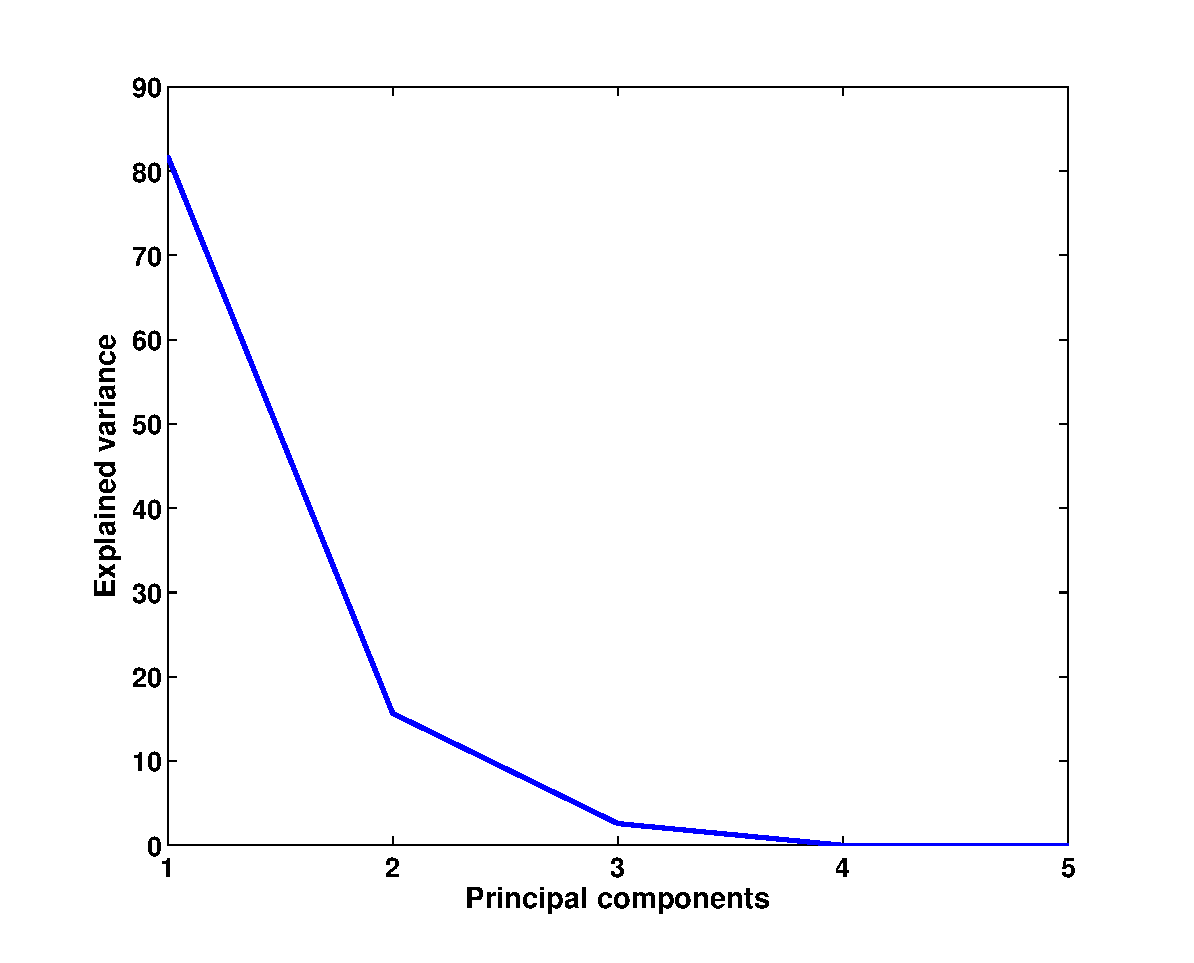
\includegraphics[width=40mm, height=35mm] {dia/clutchEV.eps}
        \label{clutchev}
      }
      \label{clutchpareto}
    \end{center}
  \end{figure}


\end{frame}


\begin{frame}
  \frametitle{Principal components of the pareto-front}
  \begin{itemize}
    \item Disk thickness and force applied are constant.
    \item Radius variables are ones in which the designs vary. 
  \end{itemize}

  \begin{table}[!ht]
    \centering
    \begin{tabular}{c|c|c|c|c|c|}
      \cline{2-6}
      & $r_{i}$ & $r_{o}$ & $ t $  & $F$ & $Z$ \\
      \hline
      \multicolumn{1}{|c|}{First PC} & 0.578 & 0.806 & 0 & 0 & 0.119\\
      \hline
      \multicolumn{1}{|c|}{Second PC} & -0.207 & 0.004 & 0 & 0 & 0.978\\
      \hline
    \end{tabular}
    \label{first2clutchPCs}
  \end{table}
\end{frame}


\begin{frame}
  \frametitle{Isomap and PCA analysis of the clusters}
  \begin{itemize}
    \item All the clusters are one-dimensional manifolds.
    \item Cluster A has two significant principal components.
  \end{itemize}

  \begin{figure}[ht]
    \begin{center}
      \subfigure[Residual variance.] {
        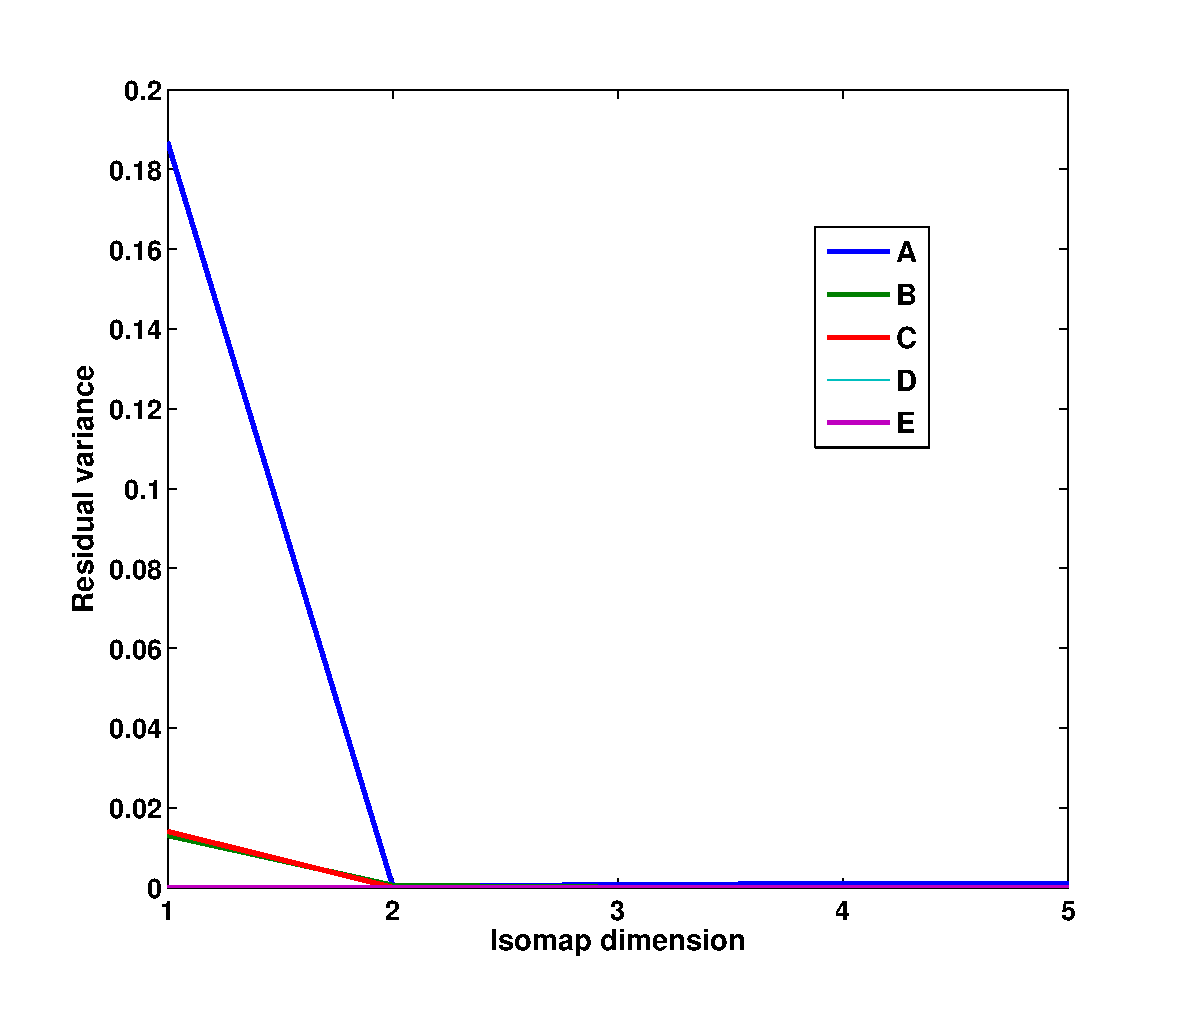
\includegraphics[width=40mm, height=35mm] {dia/clutchClustersRV.eps}
        \label{clutchcrv}
      }
      \subfigure[PCA explained variance.] {
        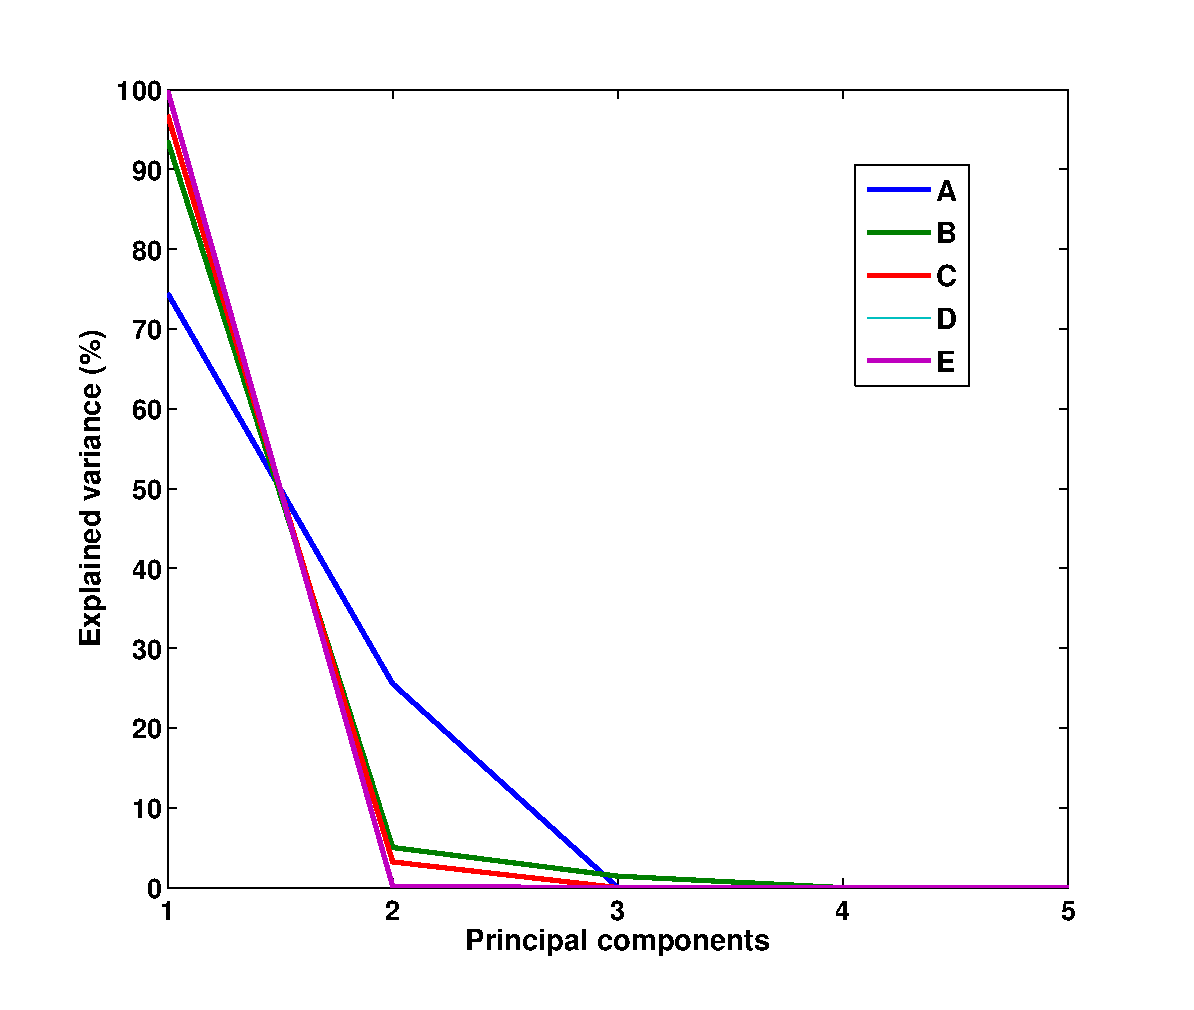
\includegraphics[width=40mm, height=35mm] {dia/clutchClustersEV.eps}
        \label{clutchev}
      }
      \label{clutchpareto}
    \end{center}
  \end{figure}


\end{frame}




\begin{frame}

  \frametitle{Significant principal components of the clusters}

  \begin{itemize}
  \item All the clusters except A are embedded in the $r_i-r_o$ plane.
  \item Cluster A has two significant principal components, first is in the 
    $r_i-r_o$ plane and the other is parallel to  $Z$.
    
  \end{itemize}



  \begin{table}[!ht]
    \centering
    \begin{tabular}{c|c|c|c|c|c|}
      \cline{2-6}
      & $r_{i}$ & $r_{o}$ & $ t $  & $F$ & $Z$ \\
      \hline
      \multicolumn{1}{|c|}{\multirow{2}{*}{\textbf{A}}} & 0.707 & 0.707 & 0 & 0 & 0\\ \cline{2-6}
      \multicolumn{1}{|c|}{}& 0 & 0 & 0 & 0 & 1\\
      \hline
      \multicolumn{1}{|c|}{\textbf{B}} & 0.236 & 0.960 & 0 & 0 & 0.146\\
      \hline
      \multicolumn{1}{|c|}{\textbf{C}} & 0.703 & 0.703 & 0 & 0 & 0.097\\
      \hline
      \multicolumn{1}{|c|}{\textbf{D}} & 0.694 & 0.719 & 0 & 0 & 0\\
      \hline
      \multicolumn{1}{|c|}{\textbf{E}} & 0.694 & 0.719 & 0 & 0 & 0\\
      \hline
      \multicolumn{1}{|c|}{\textbf{F}} & 0 & 0 & 0 & 0 & 1\\
      \hline
    \end{tabular}
    \label{first2clutchPCs}
  \end{table}


\end{frame}


\subsection{D. Welded beam design problem}





\begin{frame}[allowframebreaks]
  \frametitle{Welded beam design problem}
  
  \begin{itemize}

  \item Two objectives:
    \begin{enumerate}[(i)]
    \item Minimization of end deflection and
    \item Minimization of cost.
    \end{enumerate}
  \end{itemize}


  \begin{figure}[ht]\begin{center}
      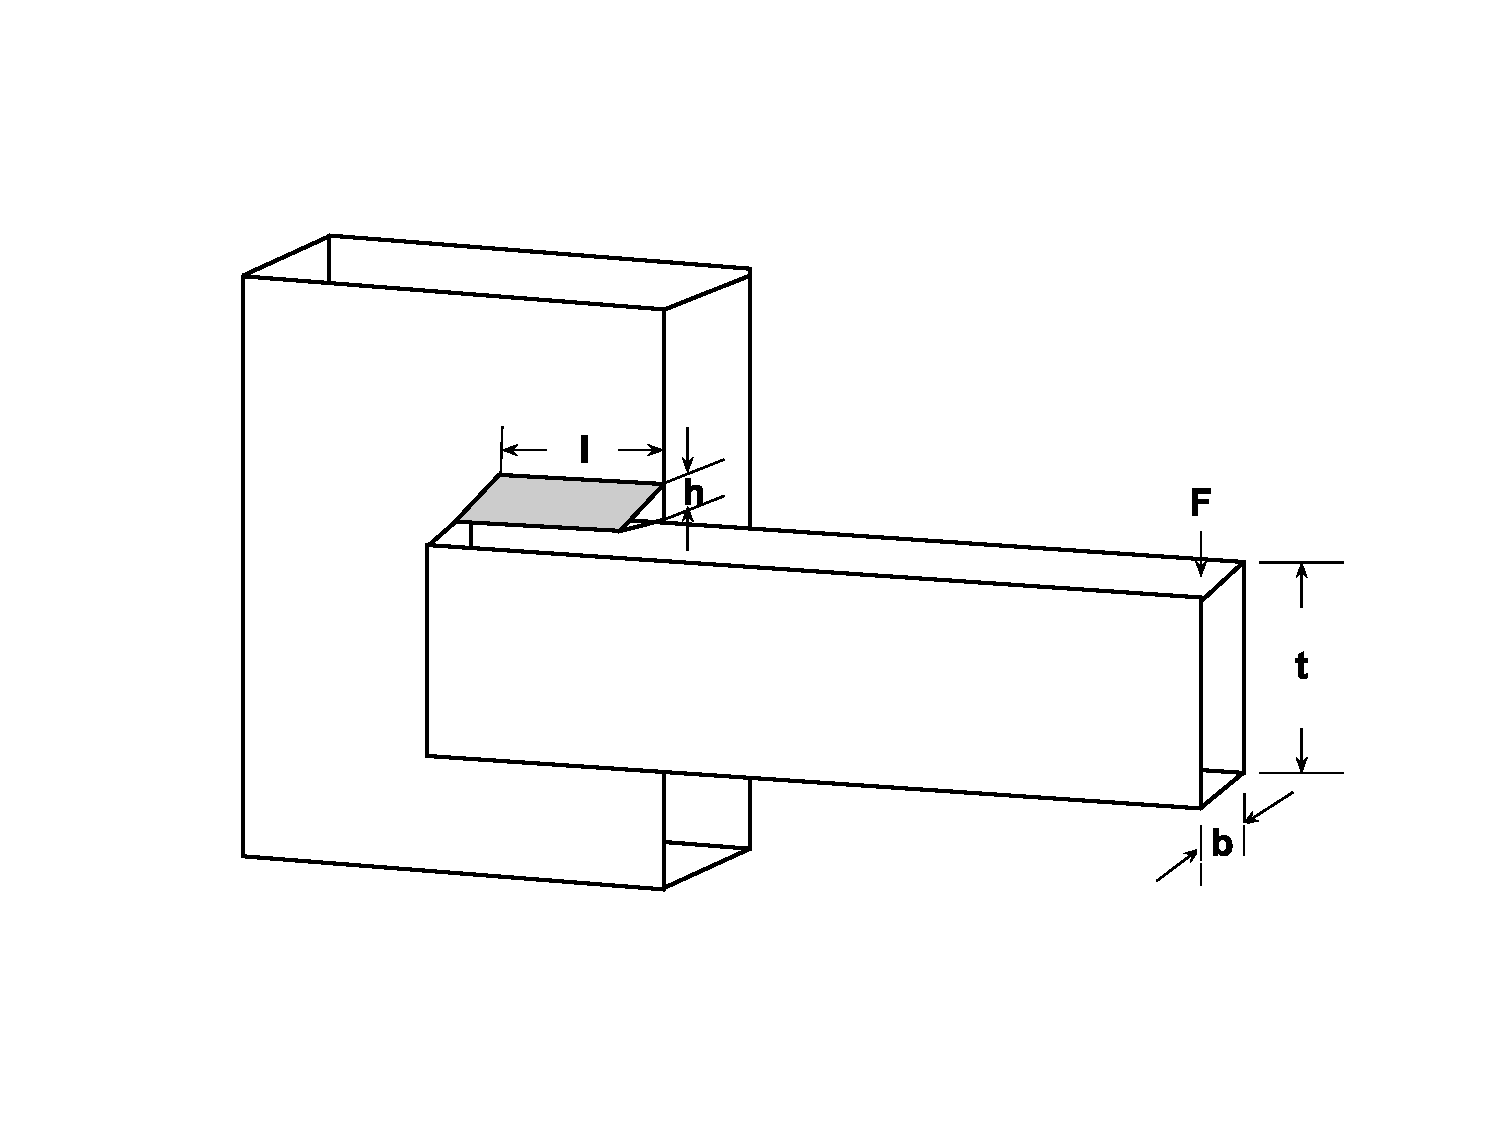
\includegraphics[width=60mm, height=40mm]{dia/wbeam.eps}
      \label{wbeam}
    \end{center}
  \end{figure}


\end{frame}





\begin{frame}
  \frametitle{Pareto-front and the clusters for welded beam design problem}

  \begin{itemize}
    \item 491 pareto-optimal solutions.
    \item 5 clusters.
  \end{itemize}

  \begin{figure}[ht]
    \begin{center}
      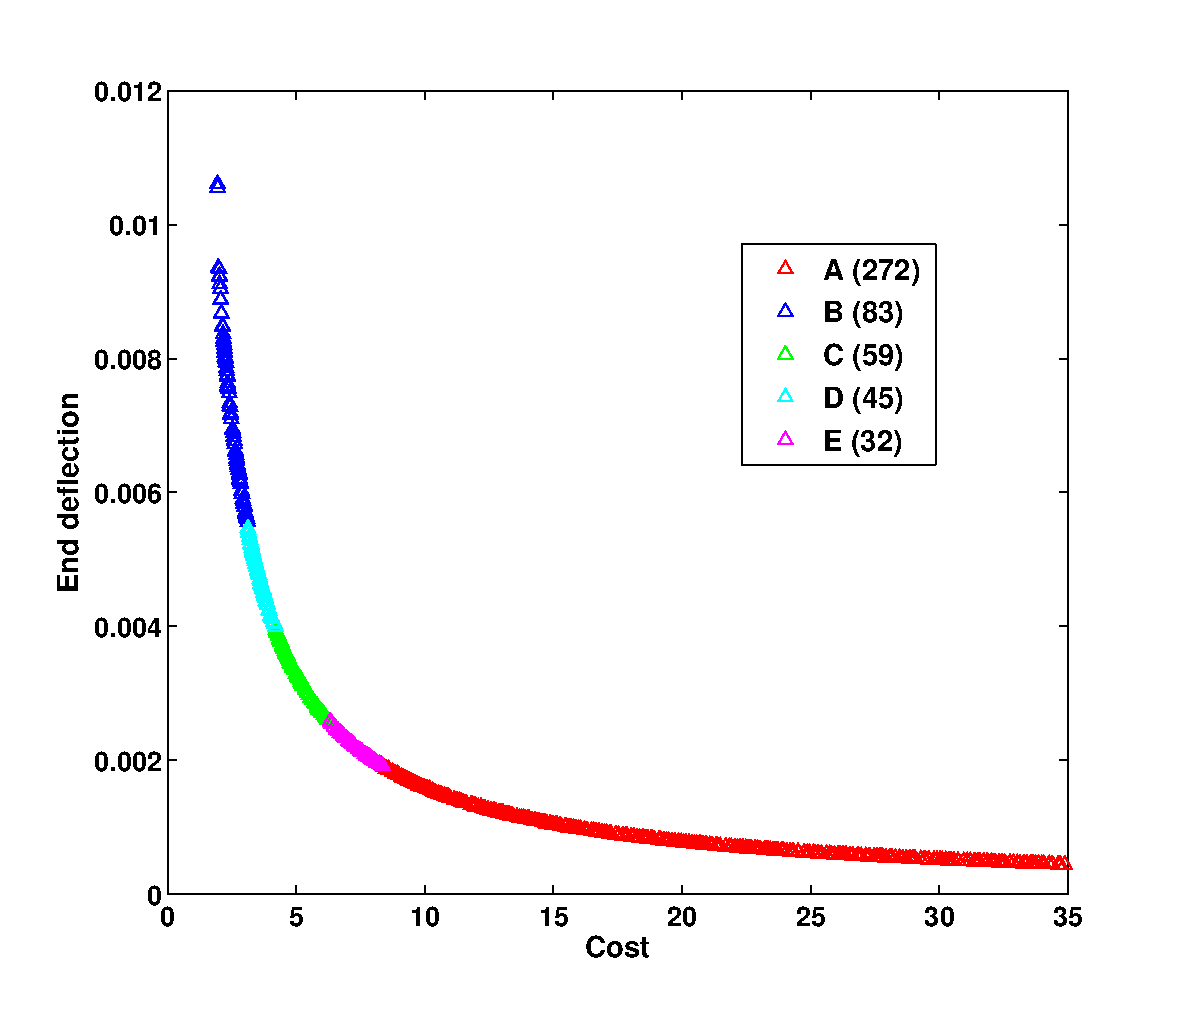
\includegraphics[width=60mm, height=50mm]{dia/wbeamParetoClusters.eps}
      \label{wbeam}
    \end{center}
  \end{figure}


\end{frame}




\begin{frame}
  \frametitle{Isomap and PCA results for the pareto-front}

  \begin{itemize}
  \item Residual variance shows a one dimensional manifold.
  \item Linear dimension is one.
  \end{itemize}
  
  \begin{figure}[ht]
    \begin{center}
      \subfigure[Residual variance.] {
        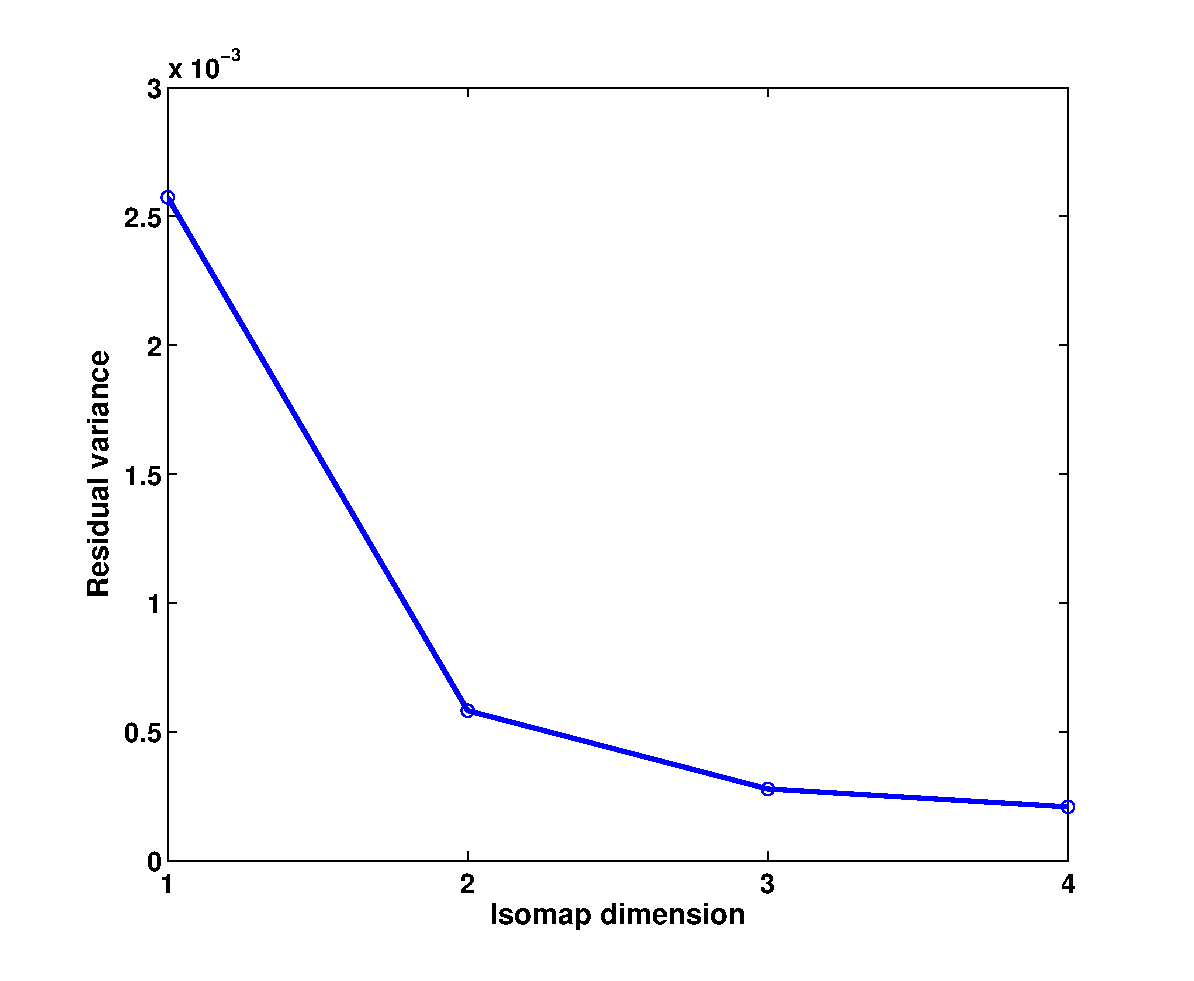
\includegraphics[width=40mm, height=35mm] {dia/wbeamWholeRV.eps}
        \label{wbeamwrv}
      }
      \subfigure[PCA explained variance.] {
        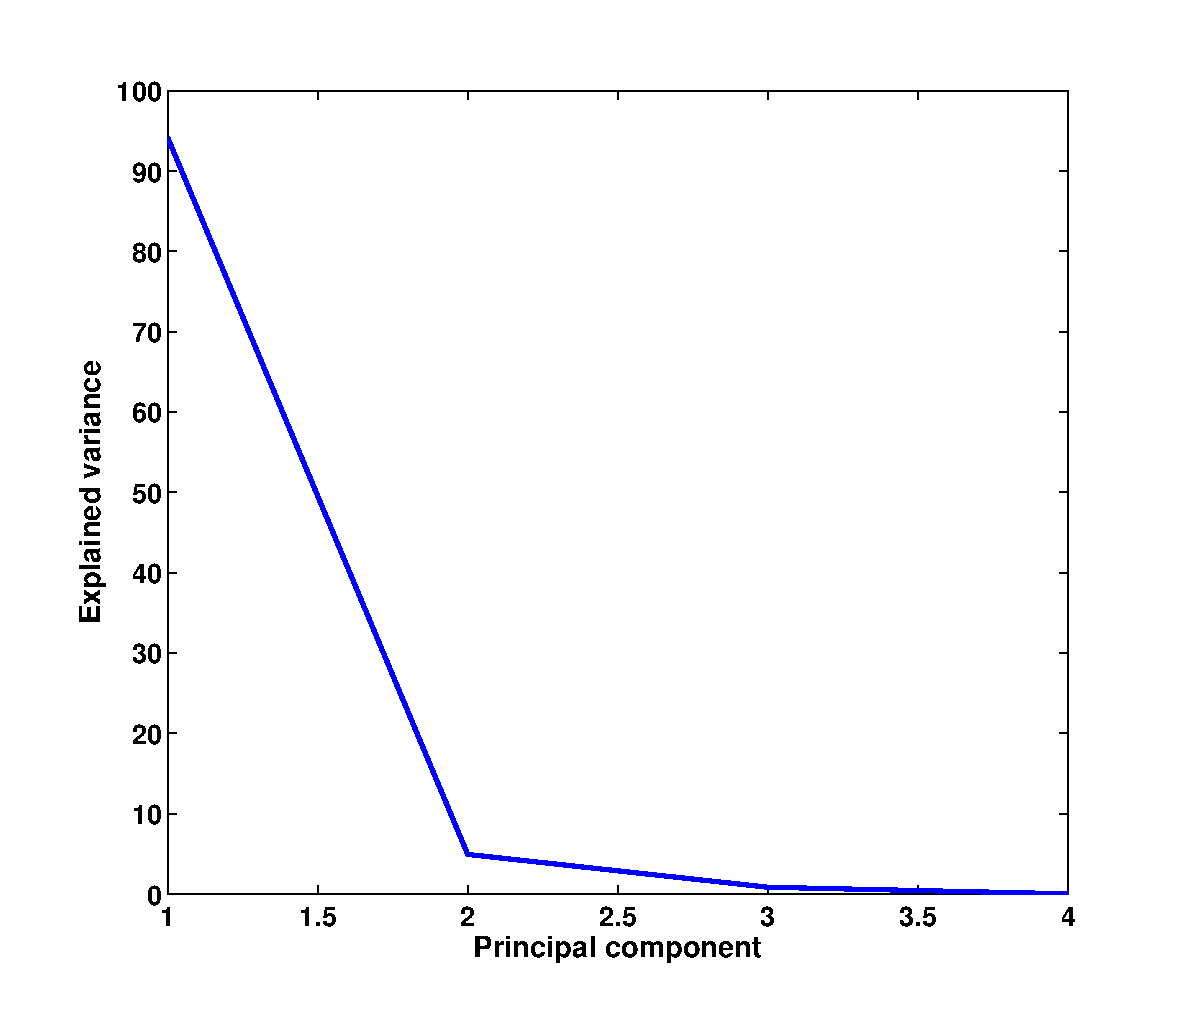
\includegraphics[width=40mm, height=35mm] {dia/wbeamWholeEV.eps}
        \label{wbeamev}
      }
      \label{wbeampareto}
    \end{center}
  \end{figure}


\end{frame}

\begin{frame}

  \frametitle{Isomap and PCA results for the clusters}
  
  \begin{itemize}
  \item All the clusters are one dimensional manifolds.
  \item Three clusters have two significant principal components, others
    have one.
  \end{itemize}

  \begin{figure}[ht]
    \begin{center}
      \subfigure[Residual variance.] {
        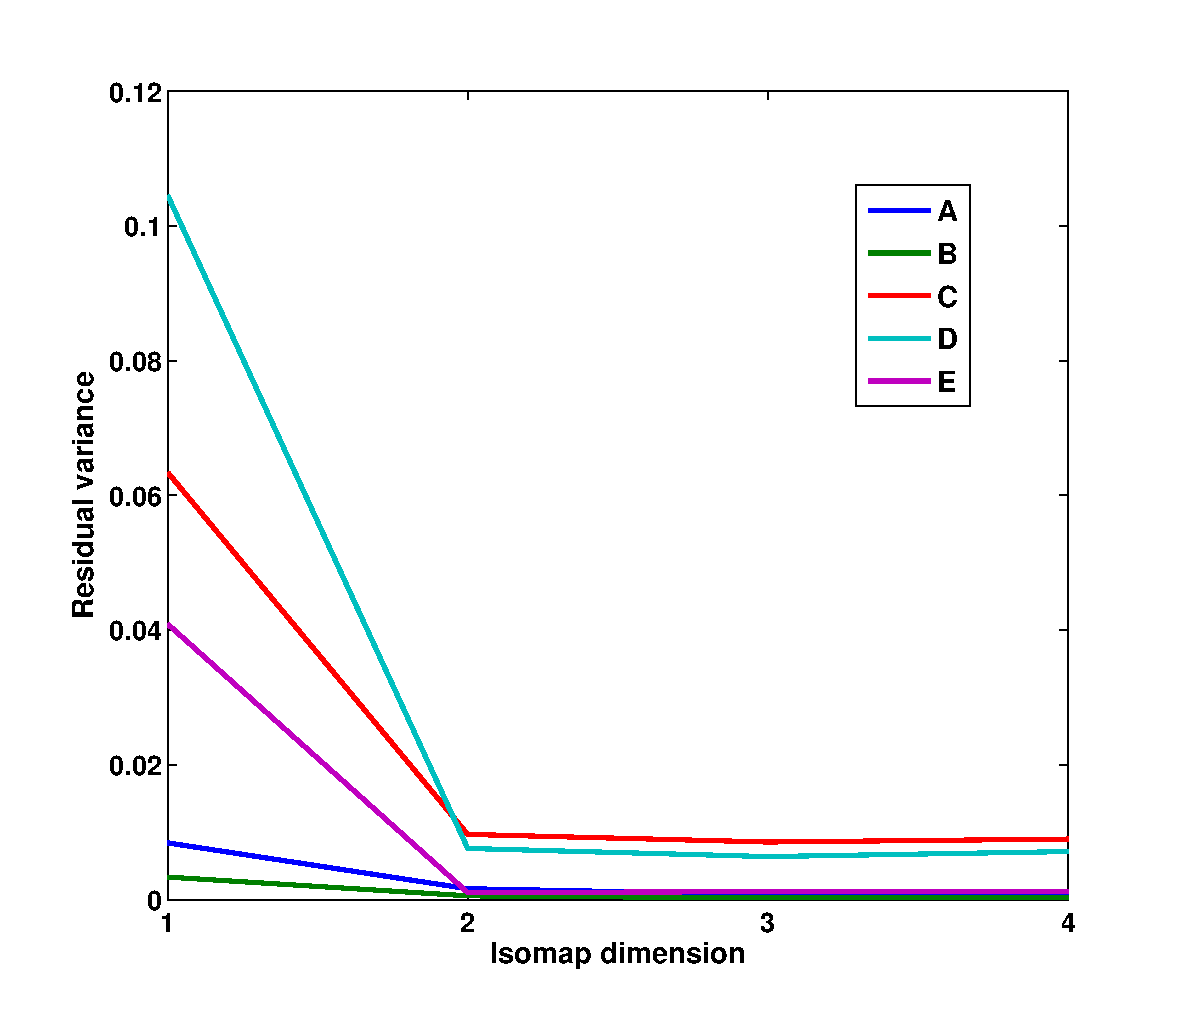
\includegraphics[width=40mm, height=35mm] {dia/wbeamClustersRV.eps}
        \label{wbeamcwrv}
      }
      \subfigure[PCA explained variance.] {
        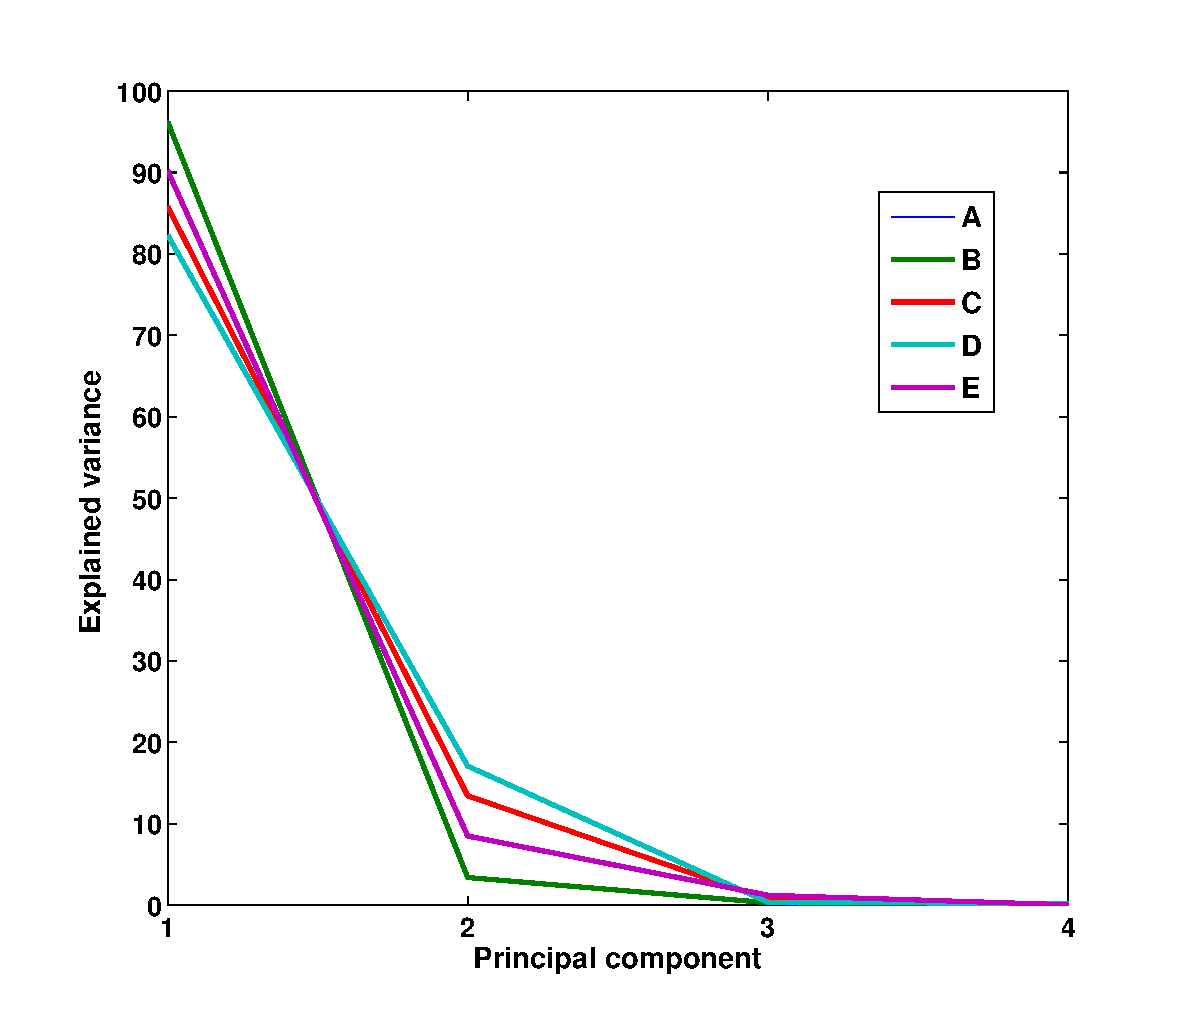
\includegraphics[width=40mm, height=35mm] {dia/wbeamClustersEV.eps}
        \label{wbeamcev}
      }
      \label{wbeampareto}
    \end{center}
  \end{figure}
\end{frame}


\begin{frame}
  \frametitle{Significant principal components of the clusters}

  \begin{itemize}
  \item The clusters having one linear dimension vary in thickness ($b$)
    and length of the weld ($l$) the most.
  \item Clusters with two principal components have significant weights in
    all variables other than width of the beam ($t$)
  \end{itemize}

  \begin{table}[!ht]
    \centering
    \begin{tabular}{c|c|c|c|c|}
      \cline{2-5}
      & $b$ & $t$ & $ l$  & $h$ \\
      \hline
      \multicolumn{1}{|c|}{\textbf{A}} & 0.965 & 0 & -0.06 & 0.249 \\
      \hline
      \multicolumn{1}{|c|}{\textbf{B}} & 0.126 & 0.068 & -0.982 & 0.115\\
      \hline
      \multicolumn{1}{|c|}{\multirow{2}{*}{\textbf{C}}} & 0.435 & 0 & -0.755 & 0.488 \\ \cline{2-5}
      \multicolumn{1}{|c|}{}& 0.897 & 0.006 & 0.404 & -0.174\\
      \hline
      \multicolumn{1}{|c|}{\multirow{2}{*}{\textbf{D}}} & 0.309 & 0 & -0.883 & 0.351 \\ \cline{2-5}
      \multicolumn{1}{|c|}{}& 0.949 & 0.011 & 0.307 & -0.06\\
      \hline
      \multicolumn{1}{|c|}{\multirow{2}{*}{\textbf{E}}} & 0.381 & 0.002 & -0.616 & 0.688 \\ \cline{2-5}
      \multicolumn{1}{|c|}{}& 0.924 & 0.019 & 0.256 & -0.282\\
      \hline
    \end{tabular}
    \label{first2wbeamPCs}
  \end{table}


% \begin{figure}[ht]\begin{center}
%  \subfloat[Isomap Residual Variances.]{
%  \label{wbeamcrv} 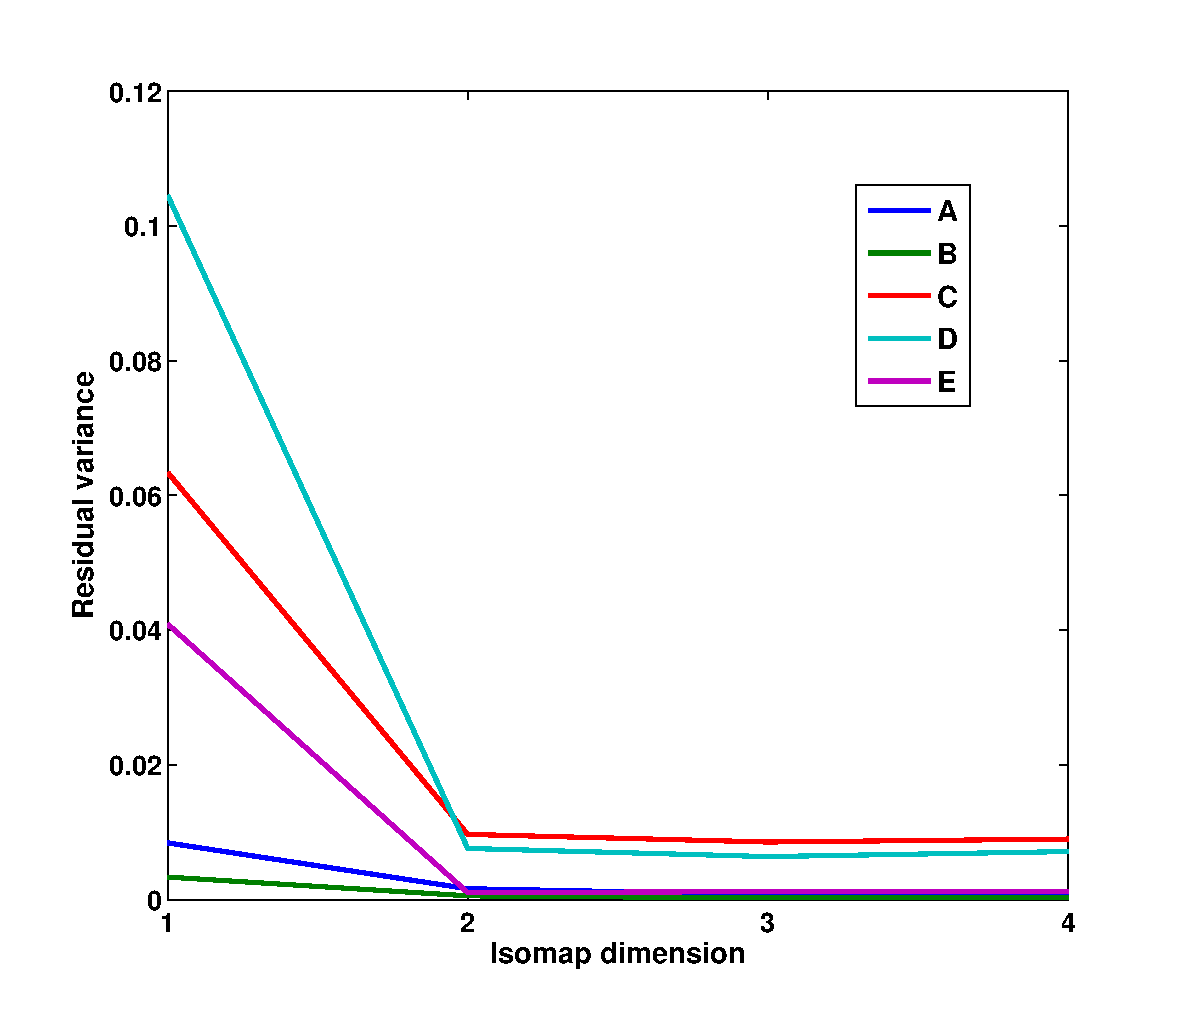
\includegraphics[width=62mm, height=52mm]{dia/wbeamClustersRV.eps}}
%  \subfloat[PCA Explained variances.]{
%  \label{wbeamcev} 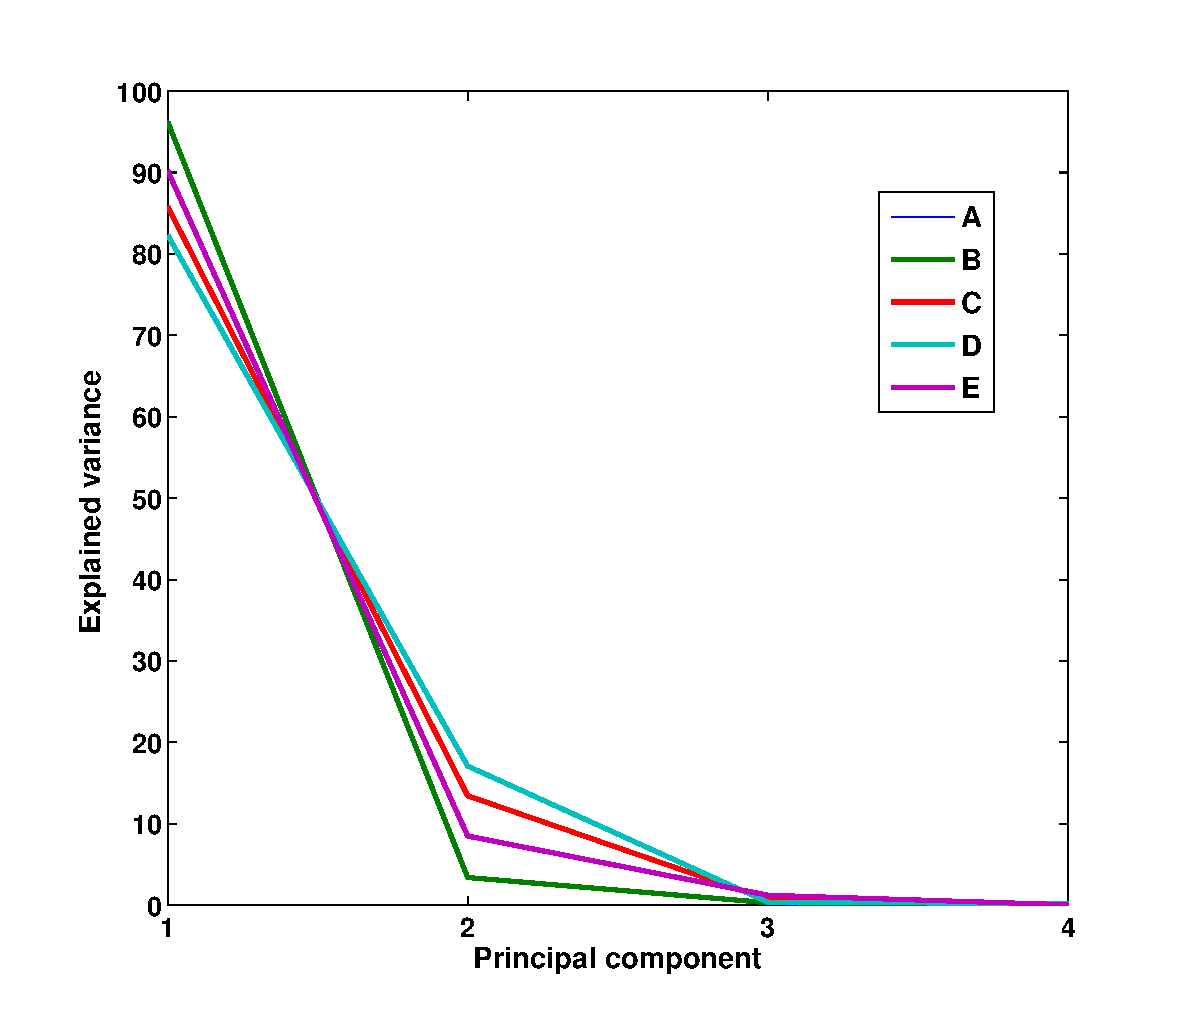
\includegraphics[width=62mm, height=52mm]{dia/wbeamClustersEV.eps}}
% \caption{Isomap and PCA results for the clusters of welded beam design
%   problem. All the clusters are one dimensional manifolds but clusters
%   \textbf{C} and \textbf{D} have two linear dimensions as they have two
%   significant components.}
%  \label{wbeamClustersVar}
% \end{center}\end{figure}



\end{frame}




\section{Conclusion}

\begin{frame}
  \frametitle{Conclusion}

  \begin{itemize}
  \item A clustering and dimensionality reduction approach to chunking in
    design.
  \item A system can be provided experience by increasing the complexity 
    of the optimization problem.
  \item Such approach to chunking is applicable in any task where task can
    be expressed as a multi-objective optimization.
  \item The example problems suggest the {\em chunk dimensionality
      conjecture}.
  \item More work is needed to substantiate the conjecture.

\end{itemize}

  

\end{frame}

\begin{frame}
\begin{center}
  Questions?
\end{center}
\end{frame}

 
\begin{frame}[allowframebreaks]
  \frametitle{References}

  \begin{thebibliography}{nevell1984unified}
    \bibitem[Bandaru and Deb, 2010]{deb10}
      Bandaru, S. and Deb, K. (2010).
      \newblock Automating discovery of innovative design principles through
      optimization.
      \newblock Technical Report 2010001, Kanpur Genetic Algorithms Laboratory,
      Indian Institute of Technology, Kanpur.


    \bibitem[Moss et~al., 2004]{moss04} Moss, J., Cagan, J., and Kotovsky,
      K. (2004).  \newblock Learning from design experience in an
      agent-based design system.  \newblock {\em Research in Engineering
        Design}, 15(2):77--92.

    \bibitem[Mukerjee and Dabbeeru, 2009]{mukerjee09} Mukerjee, A. and
      Dabbeeru, M.~M. (2009).  \newblock The birth of symbols in design.
      \newblock In {\em ASME 2009 International Design Engineering
        Technical Conferences and Computers and Information Engineering
        Conference August-September}.


  \end{thebibliography}
\end{frame}
\end{document}

